	\newcolumntype{P}[1]{>{\centering\arraybackslash}p{#1}} %para centralizar as colunas nas tabelas
	
	\thispagestyle{headfootimage}
	\section*{Introdução}
	
	Este capítulo consiste no levantamento e análise do manejo dos resíduos sólidos gerados no município de Monteiro Lobato considerando a caracterização dos resíduos segundo a origem, o volume, as formas de destinação, a disposição final adotada e os respectivos custos associados. Além disso, descreve o acondicionamento, a coleta, o transporte e o transbordo, este quando aplicável, dos seguintes tipos de resíduos:
	
	\begin{itemize}
		\item Resíduos Domiciliares;
		\item Resíduos de Limpeza Urbana;
		\item Resíduos de Estabelecimentos Comerciais e Prestadores de Serviços;
		\item Resíduos dos Serviços Públicos de Saneamento;
		\item Resíduos Industriais;
		\item Resíduos de Serviços de Saúde;
		\item Resíduos da Construção Civil;
		\item Resíduos Agrossilvipastoris;
		\item Resíduos de Serviços de Transportes; 
		\item Resíduos de Mineração; e
		\item Resíduos de Logística Reversa.
	\end{itemize}
	
	Para a elaboração deste diagnóstico, foi realizada uma reunião preliminar com a \gls{smaa}, \gls{ssm} e vice-prefeito para apresentação do objetivo da elaboração do \gls{pmgirs} de Monteiro Lobato e para compreender as responsabilidades e competências de cada secretaria. Após a reunião, foram encaminhados questionário dirigidos em forma de ofícios para as secretarias com questionamentos detalhados sobre a forma de gestão e gerenciamento dos resíduos sólidos gerados no município. As secretarias realizaram reuniões conjuntas para responder os ofícios e retornaram as respostas por meio eletrônico.
	
	A fim de complementar as informações secundárias apresentadas, foram realizadas visitas de campo acompanhadas pela \gls{smaa} para registros fotográficos do gerenciamento dos resíduos, realização de questionários estruturados para ampliar a participação dos munícipes na elaboração do \gls{pmgirs} e acompanhamento dos serviços de coleta dos resíduos comum e reciclável para determinação da rota.
	
	Os trajetos da coleta e destinação final dos resíduos foram determinados por coordenadas geográficas através do \gls{gps}, modelo Garmin etrex. Esses pontos foram inseridos no software ArcGIS e sobrepostos ao mapa da região.
	
	O questionário estruturado foi aplicado aos estabelecimentos comerciais responsáveis pela geração de óleos lubrificantes e pneus cujos endereços foram disponibilizados pela Prefeitura. O questionário foi realizado para conhecimento da geração e destinação final destes resíduos que devem apresentar sistema de logística reversa de acordo com o artigo 33 da Lei nº 12.305, de 02 de agosto de 2010.
	
	O município de Monteiro Lobato não dispõe de recurso específico destinado para o gerenciamento dos resíduos sólidos e de limpeza urbana. Neste contexto, foi solicitado à \gls{ssm}, via ofício, os custos associados para todas atividades do manejo de resíduos sólidos e serviços de limpeza urbana em relação aos salários dos funcionários, manutenção de equipamentos, contratos com empresas terceirizadas e gastos com transporte.
	
	A \gls{ssm} repassou um documento em formato .pdf com a relação de funções e atividades de vinte e nove funcionário e a folha de ponto. A fim de estimar qual o custo dos funcionários para a prefeitura em cada atividade de manejo de resíduos sólidos e de serviços de limpeza urbana, o valor total do salário base foi somado aos descontos pagos pela prefeitura (imposto de renda, \gls{inss} e demais contribuições) e ao \gls{fgts} e este total foi dividido entre os vinte e nove funcionários.
	
	Dependendo do cargo, das atribuições e das horas extras realizadas, a prefeitura ainda arca com uma base variável mensal em relação aos funcionários referente ao pagamento de horas extras e Salário-família. De acordo com a descrição da folha de pagamento disponibilizada, esta base variável é de aproximadamente R\$ 7.202,37 ao mês.
	
	Além disso, o município dispõe de cinco funcionários do Programa Frente de Trabalho, que qualifica profissionalmente e gera renda para cidadãos que se encontram desempregados e em situação de alta vulnerabilidade social, para colaboração em serviços de limpeza urbana, serviços de manutenção e serviços braçais. A estimativa do valor destinado a estes funcionários foi realizada considerando o salário base e o valor da cesta básica que o município disponibiliza para os funcionários.
	
	A partir do diagnóstico de resíduos sólidos é possível desenvolver um sistema de cálculo específico de custos dos serviços de limpeza urbana e de manejo de resíduos sólidos. A partir disso e da elaboração efetiva do \gls{pmgirs} de Monteiro Lobato, o município tem direito a ter acesso a recursos da União destinados para serviços relacionados a limpeza urbana e ao manejo de resíduos sólidos, de acordo com o artigo 18 da \gls{pnrs} \cite{brasil:12305}.
	
	O diagnóstico da situação de resíduos no município de Monteiro Lobato é indispensável para a definição de futuras diretrizes, identificação de gerenciamento inadequados, para o levantamento de ações mitigadoras e preventivas e para a elaboração de prognóstico \cite{brasil:11445}. Além disso, o levantamento do diagnóstico é de suma importância para a elaboração de propostas que visem a utilização racional de recursos ambientais, a redução de desperdícios, a minimização da geração de resíduos sólidos e o manejo ambientalmente adequado e economicamente viável.

\newpage
	
	\section{Diagnóstico do sistema de limpeza urbana e manejo de resíduos sólidos}
	
	De forma resumida, o artigo 13 da Lei nº 12.305, de 02 de agosto de 2010 classifica os resíduos sólidos como:
	
	\begin{description}
		\item[\gls{rd}] originários de atividades domésticas em residências urbanas;
		\item[\gls{rlu}] originários da varrição, limpeza de logradouros e vias públicas e outros serviços de limpeza urbana;
		\item[\gls{rsu}] englobados nos resíduos domiciliares e nos resíduos de limpeza urbana;
		\item[\gls{rc}] gerados nessas atividades, exceto os serviços de limpeza urbana, de saneamento básico, de saúde, de construção civil e de transportes;
		\item[\gls{rspsb}] gerados nessas atividades, exceto os resíduos sólidos urbanos;
		\item[\gls{ri}] gerados nos processos produtivos e instalações industriais;
		\item[\gls{rss}] gerados nos serviços de saúde, conforme definido em regulamento ou em normas estabelecidas pelos órgãos do \gls{sisnama} e do \gls{snvs};
		\item[\gls{rcc}] gerados nas construções, reformas, reparos e demolições de obras de construção civil, incluídos os resultantes da preparação e escavação de terrenos para obras civis;
		\item[\gls{ra}] gerados nas atividades agropecuárias e silviculturais, incluídos os relacionados a insumos utilizados nessas atividades;
		\item[\gls{rst}] originários de portos, aeroportos, terminais alfandegários, rodoviários e ferroviários e passagens de fronteira;
		\item[\gls{rm}] gerados na atividade de pesquisa, extração ou beneficiamento de minérios;
		\item[\gls{rlr}] gerados após o uso pelo consumidor dos materiais provindos de fabricantes, importadores, distribuidores e comerciantes de agrotóxicos e suas embalagens, pilhas e baterias, óleos lubrificantes e suas embalagens, lâmpadas fluorescentes de vapor de sódio e mercúrio e de luz mista, produtos eletroeletrônicos e seus componentes.
		
	\end{description}
	
	\subsection{Resíduos Sólidos Urbanos}
	Os \gls{rsu} compreendem os resíduos domiciliares e os resíduos de limpeza urbana. Os resíduos domiciliares são os resíduos originários de atividades domésticas em residências urbanas. Os resíduos de limpeza urbana englobam os resíduos originários de varrição, de limpeza de logradouros, de vias públicas e de capina e poda \cite{brasil:12305, brasil:11445}.
	
	Além disso, nos casos em que os resíduos de estabelecimentos comerciais e prestadores de serviços são caracterizados como não perigosos, o poder público pode classificá-los como resíduos equivalentes aos resíduos domiciliares \cite{brasil:12305}.
	
	A geração estimada pela \gls{abrelpe} de  no Brasil foi de 78,3 milhões de toneladas em 2016, considerando a soma das projeções de cada região do país. Já a geração per capita apresentou um valor de aproximadamente 1,04 kg por habitante por dia \cite{abrelpe_panorama_2016}.
	
	Em relação a cobertura de coleta, o \gls{ipea} publicou em 2012 uma relação da coleta direta e indireta em área urbana e rural de resíduos sólidos urbanos entre os anos de 2000 e 2008 (\autoref{tab:cobertura_coleta}).
	
	\input{./produtos/prodtres/cobertura_coleta}
	
	Analisando a \autoref{tab:cobertura_coleta} é possível verificar que a distribuição da taxa de cobertura de coleta de \gls{rsu} não é uniforme entre as regiões do país. Apesar de a coleta em área rural ter duplicado de 2000 a 2008 em porcentagem, a cobertura é muito baixa, sendo apenas 32,7 \% no país \cite{ipea_diagrsu_2012}.
	
	As regiões Sudeste e Sul apresentaram a maior cobertura em área rural no ano de 2008, porém esses valores representam apenas 50 \% dos domicílios. Já a cobertura na área urbana apresenta valores acima de 95 \% de abrangência para todas as regiões do país. No entanto, o índice de coleta total das regiões Norte, Nordeste e Centro-Oeste ainda possuem deficiência \cite{ipea_diagrsu_2012}.
	
	Em 2016, de acordo com as estimativas da \gls{abrelpe}, o índice de cobertura de coleta de \gls{rsu} do país cresceu para 91 \% e os índices da região Norte, Nordeste, Centro-Oeste, Sudeste e Sul aumentaram para, respectivamente, 81 \%, 79 \%, 94 \%, 98 \% e 95 \% \cite{abrelpe_panorama_2016}. Comparando as estimativas de 2008 da \autoref{tab:cobertura_coleta} com as de 2016, a abrangência de coleta de \gls{rsu} foi ampliada, porém, a distribuição ainda não é equivalente entre todas as regiões.
	
	Tratando-se de disposição final no Brasil referente aos resíduos sólidos domiciliares e/ou urbanos, a sua relação e diferentes formas são apresentadas na \autoref{fig:image004}, com dados de tonelada por dia para o ano de 2008.A disposição final mais utilizada no Brasil, assim como pode ser observado na \autoref{fig:image004}, ainda se trata dos aterros sanitários. 
	
	\begin{figure}
		\centering
		\includegraphics[width=0.75\linewidth]{produtos/prodtres/image004}
		\caption{Relação de disposição final dos \gls{rsu} no Brasil em 2008}
		\legend{Fonte: Adaptado de \cite{ipea_diagrsu_2012}}
		\label{fig:image004}
	\end{figure}
	
	A definição de um aterro sanitário, de acordo com a \gls{nbr} 8419/92, é uma técnica de disposição de resíduos sólidos urbanos no solo, sem causar danos à saúde pública e à sua segurança minimizando os	impactos ambientais, método este que utiliza os princípios de engenharia (impermeabilização do solo, cercamento, ausência de catadores, sistema de drenagem de gases, águas pluviais e lixiviado) para confinar os resíduos e rejeitos à menor área possível e reduzi-los ao menor volume permissível, cobrindo-o com uma camada de terra na conclusão de cada jornada de trabalho, ou a intervalos menores, se necessário \cite{abnt:8419}.

	Já o aterro controlado, definido pela \gls{pnrs}, é uma forma inadequada de disposição final de resíduos e rejeitos, no qual o único cuidado realizado é o recobrimento da massa de resíduos e rejeitos com terra. O lixão é uma forma inadequada de disposição final de resíduos e rejeitos, que consiste na descarga do material no solo sem qualquer técnica ou medida de controle \cite{brasil:12305}.

	Estima-se que, em 2016, 58,4 \% de \gls{rsu} do montante total do país tenha sido destinado a aterros sanitários, enquanto que 24,2 \% foi disposto em aterro controlado e 17,4 \% em lixões \cite{abrelpe_panorama_2016}. Neste contexto, é possível aferir que não houve significativa evolução em relação a disposição ambientalmente adequada dos resíduos sólidos no país.
	
	Apesar do Brasil ter um grande número de municípios contemplados com a disposição final dos \gls{rsu} em aterros sanitários, isso representa 40,20 \% do total, ou seja, menos da metade dos municípios brasileiros possuem aterros considerados sanitários. Quando se fragmenta essa distribuição por regiões, percebe-se que as regiões Norte e Nordeste possuem um maior número de locais com disposição final ambientalmente inadequadas (\autoref{fig:image005}). A região Centro-Oeste apresenta uma relação numericamente comparável entre as formas atualmente adotadas de disposição final. As regiões Sudeste e Sul têm as melhores condições quanto à disposição final dos \gls{rsu}, e possui lixões em 10 \% e 12 \% dos municípios, respectivamente.
	
\begin{figure}
	\centering
	\includegraphics[width=0.75\linewidth]{produtos/prodtres/image005}
	\caption{Relação de disposição final dos \gls{rsu} por município no Brasil e suas regiões.}
	\legend{Fonte: Adaptado de \cite{abrelpe_panorama_2016}}
	\label{fig:image005}
\end{figure}

	O serviço público é responsável pela gestão e gerenciamento dos serviços de limpeza urbana e pelo manejo dos resíduos domiciliares, de modo a atender ao plano municipal de gestão integrada de resíduos sólidos \cite{brasil:12305}.
	
	Se o poder público classificar os resíduos de estabelecimentos comerciais e prestadores de serviço como equivalentes à resíduos domiciliares, o gerenciamento será de responsabilidade do poder público. No entanto, se os resíduos de estabelecimentos comerciais e prestadores de serviço forem caracterizados como perigosos ou não forem equiparados à resíduos domiciliares por sua natureza, composição, volume ou quantidade superior a determinada pelo município, os geradores estarão sujeitos a elaborar o próprio plano de gerenciamento \cite{brasil:12305}.
	
	No município de Monteiro Lobato os \gls{rsu} são divididos em duas categorias: resíduos sólidos comuns e resíduos sólidos recicláveis. Os resíduos sólidos comuns no município consistem em resíduos considerados domiciliares (com exceção de recicláveis), rejeitos e matéria orgânica. 
	
	Os resíduos oriundos de serviços de limpeza urbana como varrição, desobstrução de sarjetas, poda e capina são usualmente considerados pelo município como resíduos comuns e recebem, em sua maioria, a mesma destinação e disposição final que os resíduos domiciliares e de estabelecimentos comerciais e prestadores de serviços.
	
	Os resíduos sólidos recicláveis são constituídos de materiais plásticos de diversas categorias (PET, PP, PEBD, PEAD entre outros), vidro, metal, papel e papelão, possuem valor agregado e devem voltar ao sistema produtivo como matéria prima para fabricação de novos produtos através da reciclagem e/ou reaproveitamento.
	
	\subsection{Resíduo Sólido Comum}
	
	Em relação à cobertura de coleta de \gls{rsu} do município de Monteiro Lobato, a \autoref{tab:pop_atendida} apresenta a relação entre população (total, urbana e rural) atendida pelo serviço de coleta, dados disponibilizados entre 2009 e 2015 \cite{snis_serie_2019_2015}.

	\input{./produtos/prodtres/pop_atendida}
	
	Ao analisar a \autoref{tab:pop_atendida} verifica-se a deficiência na declaração dos dados pelos municípios para o \gls{snis}. A ausência de dados consistentes ao longo da Série Histórica prejudica a interpretação e expõe uma fragilidade em relação a qualidade das informações.
	
	Considerando-se a fragilidade dos dados de cobertura de coleta, as discussões serão baseadas principalmente nas informações prestadas pela autoridade pública municipal de Monteiro Lobato.
	
	Os dados obtidos sobre os resíduos comuns foram coletados em três etapas. Primeiro foram encaminhados questionários dirigidos em forma de ofício para \gls{smaa} bem como para a \gls{ssm} e separados por origem de resíduos: \gls{rsu}, \gls{rss}, \gls{rcc}. Nesse questionário foi indagado sobre as condições de coleta, equipamentos utilizados, número de funcionários responsáveis pelas atividades, custo associado, destinação e disposição final dos resíduos.
	
	Em seguida, na segunda etapa através da ferramenta Excel 2016, foram realizadas avaliações estatísticas dos dados de disposição final destes resíduos no aterro sanitário de Tremembé administrado pela companhia ESTRE-Resicontrol, que forneceu uma série histórica entre 2 de janeiro de 2014 até 9 de outubro de 2017.
	
	Por fim, foram realizados registros fotográficos das formas de acondicionamento dos resíduos comum e dos equipamentos e materiais utilizados, a fim de validar as respostas dos questionários dirigidos.
	
	\subsubsection{Acondicionamento}
	
	De acordo a \gls{ssm}, o acondicionamento coletivo de resíduos comuns no município é composto por 59 lixeiras. Os resíduos comuns domiciliares e comerciais ficam normalmente armazenados em lixeira de ferro de, aproximadamente, 2 x 1 x 1 metros, como apresentado na parte superior da \autoref{fig:image006}. Existem também as lixeiras de madeira, que apresentam dimensões de 2 x 1 x 1 m ou de 1,20 x 1 x 1 m (parte inferior da \autoref{fig:image006}). Foi possível verificar que, apesar de as lixeiras apresentarem um volume significativo, alguns resíduos são dispostos inadequadamente no solo ao lado das lixeiras. 
	
	\begin{figure}
		\centering
		\includegraphics[width=0.7\linewidth]{produtos/prodtres/image006}
		\caption{Lixeira de ferro e de madeira}
		\legend{Fonte: Elaborado pelos autores}
		\label{fig:image006}
	\end{figure}
	
	Os resíduos introduzidos nas lixeiras são embalados pelos munícipes em sacolas de supermercado, saco plástico pretos de volumes distintos, caixas de papelão entre outros materiais. Entretanto, muitos resíduos sólidos são dispostos nas lixeiras sem o devido acondicionamento, o que prejudica o processo de coleta por parte dos funcionários, como mostrado na \autoref{fig:image007}
	
	\begin{figure}
		\centering
		\includegraphics[width=0.7\linewidth]{produtos/prodtres/image007}
		\caption{Lixeira de ferro e formas de acondicionamento}
		\legend{Fonte: Elaborado pelos autores}
		\label{fig:image007}
	\end{figure}
		
		 	
	As lixeiras maiores costumam compor as áreas comuns dos bairros, no entanto, alguns moradores possuem o próprio cesto de lixo, como exemplificado pela \autoref{fig:image008}. Existe ainda o hábito de alguns moradores pendurarem sacos plásticos com os resíduos em ganchos no portão da residência, como apresentado na \autoref{fig:image009}.
	
	\begin{figure}
		\centering
		\includegraphics[width=0.5\linewidth]{produtos/prodtres/image008}
		\caption{Cesto de armazenamento de resíduos}
		\legend{Fonte: Elaborado pelos autores}
		\label{fig:image008}
	\end{figure}	
		
				
	\begin{figure}
		\centering
		\includegraphics[width=0.5\linewidth]{produtos/prodtres/image009}
		\caption{Sacos pendurados em ganchos}
		\label{fig:image009}
		\legend{Fonte: Elaborado pelos autores}
	\end{figure}
		
			
	\subsubsection{Coleta, transbordo e transporte}
	
	Os resíduos comuns coletados no município são compostos por resíduos sólidos produzidos por estabelecimentos comerciais e prestadores de serviço, residências de área urbana e área rural, resíduos de caráter domiciliar não reciclável de estabelecimentos particulares geradores de \gls{rss}, \gls{rst} e \gls{ri}, além de parte dos resíduos oriundos da limpeza pública. Essa abrangência na coleta ocorre devido à inexistência de regulamentação pelo município quanto ao tipo de gerador e suas obrigações legais conforme preconiza a \gls{pnrs} (Lei nº 12.305 de 2010).
	
	A coleta municipal dos resíduos sólidos comuns ocorre às segundas, terças, quintas e sextas-feiras, de acordo com os horários apresentados na \autoref{tab:dias_coleta}.  O município dispõe de um caminhão do tipo compactador DMN 2206 de 9,29 m$^{3}$ com o qual é realizada a coleta.
	
	\input{./produtos/prodtres/dias_coleta}
	
	Das 59 lixeiras coletivas existentes no município e conforme descrição da \gls{ssm}, o caminhão coletor passa pelos seguintes bairros com respectivos números de lixeiras coletivas após sair da \gls{ssm}:

	\begin{itemize}
		\item SP 50 Bairro Taquari – 4 lixeiras; 
		\item Bairro Descoberto – 1 lixeira; 
		\item Bairro Ponte Nova – 3 lixeiras; 
		\item Estrada do Livro – 2 lixeiras; 
		\item Bairro Pedra Branca – 5 lixeiras; 
		\item Estrada São Francisco – 6 lixeiras; 
		\item Centro – 12 lixeiras; 
		\item Bairro Alpes do Boquira – 1- lixeira; 
		\item SP 50 Bairro São Benedito – 13 lixeiras; 
		\item Estrada Ito Rennó – 2 lixeiras; 
		\item Estrada Cruzeiro – 1 lixeira; 
		\item Bairro do Souzas – 4 lixeiras; 
		\item Estrada Fabiano – 2 lixeiras; 
		\item Estrada Pandavas – 3 lixeiras.
	\end{itemize}

	Durante o percurso realizado em uma segunda-feira foram obtidas as coordenadas geográficas das lixeiras cujo resíduo sólido comum foi recolhido através do \gls{gps}. A rota dessa coleta passou por 37 lixeiras cujas localizações são apresentadas na \autoref{fig:image012}. 
	
	\begin{figure}
		\centering
		\includegraphics[width=1\linewidth]{produtos/prodtres/image012}
		\caption{Localização de 37 lixeiras coletivas cuja coleta de segunda feira recolheu o resíduo sólido comum.}
		\legend{Fonte: Elaborado pelos autores.}
		\label{fig:image012}
	\end{figure}
	
	A coleta dos pontos geográficos das lixeiras ocorreu juntamente com o registro fotográfico de cada local.  Durante o percurso, notou-se que em alguns pontos há o descarte, em local inadequado, do líquido acumulado no caminhão compactador, conforme ilustra a \autoref{fig:image013}.
	
	\begin{figure}
		\centering
		\includegraphics[width=0.7\linewidth]{produtos/prodtres/image013}
		\caption{Remoção do liquido existente no caminhão compactador.}
		\legend{Fonte: Elaborado pelos autores.}
		\label{fig:image013}
	\end{figure}
	
	Para a retirada dos resíduos das lixeiras é feita uma manobra com o caminhão, em que o mesmo se aproxima de ré até ficar bastante próximo da lixeira, como ilustram as \autoref{fig:image014} e \autoref{fig:image015}. A \autoref{fig:image015} também mostra a disposição inadequada dos resíduos sólidos no solo, fora da lixeira.
	
	\begin{figure}
		\centering
		\includegraphics[width=0.7\linewidth]{produtos/prodtres/image014}
		\caption{Retirada de resíduos de lixeira pública.}
		\label{fig:image014}
		\legend{Fonte: Elaborado pelos autores.}
	\end{figure}
	
	\begin{figure}
		\centering
		\includegraphics[width=0.50\linewidth]{produtos/prodtres/image015}
		\caption{Retirada de resíduos de lixeira pública.}
		\label{fig:image015}
		\legend{Fonte: Elaborado pelos autores.}
	\end{figure}
	
	Em dezembro de 2017, o percurso do caminhão coletor foi acompanhado durante alguns dias da semana e sua rota registrada através do \gls{gps}. A obtenção dessas rotas colabora com o possível traçado de caminhos mais otimizados, e assim, o município teria um transporte mais rápido e com menor consumo de combustível, gerando menor custo e menor emissão de gases de efeito estufa.
	
	Para os dias de coleta de resíduo comum (segunda, terça, quinta e sexta-feira), não há uma rota pré-definida pela secretaria, ficando a critério do motorista responsável contanto que atenda a todos os locais em que a coleta deve ser realizada. A \autoref{fig:image016} apresenta o percurso realizado referente à uma quinta-feira.
	
	\begin{figure}
		\centering
		\includegraphics[width=1\linewidth]{produtos/prodtres/image016}
		\caption{Rota da coleta de resíduo comum no município na quinta-feira no período da manhã.}
		\label{fig:image016}
		\legend{Fonte: Elaborado pelos autores.}
	\end{figure}
	
	De acordo com informações da \gls{ssm}, a partir de 2019, após finalizada a coleta dos resíduos comuns às 16 horas (às segundas, terças, quintas e sextas-feiras,), o caminhão segue em direção ao aterro sanitário de Tremembé para a devida disposição final. O percurso realizado até o aterro sanitário é de aproximadamente 48 km \autoref{fig:image017}.
	
	\begin{figure}
		\centering
		\includegraphics[width=1\linewidth]{produtos/prodtres/image017}
		\caption{Localização de Monteiro Lobato em relação ao aterro sanitário de Tremembé.}
		\label{fig:image017}
		\legend{Fonte: Elaborado pelos autores.}
	\end{figure}
	
	
	Nesses dias em que o resíduo é encaminhado ao aterro sanitário, a média diária que o caminhão percorre é de 207,7 km para realização da coleta, transporte e retorno à base. Para execução da coleta o município dispõe de três funcionários, sendo um motorista e dois coletores.
	
	\subsubsection{Disposição final}
	
	O aterro sanitário de Tremembé pode receber resíduos Classe I, II A e II B. Ao chegar, o caminhão passa por uma balança rodoviária para aferição de sua massa e posteriormente o resíduo é encaminhado para o local de despejo onde é finalmente disposto em local adequado. Em seguida, o caminhão retorna à balança para aferir novamente sua massa.
	De uma forma geral, o sistema de coleta de resíduos comuns pode ser esquematizado conforme a \autoref{fig:image017a}.
	
	\begin{figure}
	\centering
	
\includegraphics[width=0.75\linewidth]{produtos/prodtres/image017a}
	\caption{Gerenciamento dos resíduos comum por Monteiro Lobato Fonte: Elaborado pelos autores.}
	\label{fig:image017a}
	\legend{Fonte: Elaborado pelos autores.}
\end{figure}
	
	\subsubsection{Volume}
	
	Através da avaliação da série histórica dos dados cedidos pelo aterro sanitário de Tremembé, foi possível aferir algumas características existentes no município e sua dinâmica. O conhecimento desses dados é importante para entender o comportamento de geração de resíduos sólidos comuns, e assim elaborar ações e metas que auxiliem na melhoria da gestão dos resíduos.
	
	Nessa avaliação procurou-se conhecer a variação de geração do resíduo ao longo dos meses, onde foi possível perceber que, entre os anos avaliados, ocorreu uma tendência de maior geração entre os meses de dezembro e março, sendo janeiro o mês mais expressivo ao longo dos anos. Uma hipótese para explicar esse fato seria o acréscimo do número de turistas na região, no período.
	
	Há também um período de menor geração que ocorre entre agosto e setembro, conforme \autoref{fig:image018}. No Apêndice A consta a geração pontual que cada segunda, quarta e sexta feira produzia ao longo dos meses comparativamente com as médias anuais e diárias ao longo dos anos avaliados (2014-2017).

\begin{landscape}	
	\begin{figure}
		\centering
		\includegraphics[width=1\linewidth]{produtos/prodtres/image018}
		\caption{Geração total em tonelada de resíduo comum de Monteiro Lobato por mês.}
		\legend{Fonte: ESTRE-Resicontrol, adaptado.}
		\label{fig:image018}
	\end{figure}
\end{landscape}
	
	Nessa avaliação também foi possível obter e compreender como é a dinâmica de produção do resíduo comum pelos munícipes. Neste caso percebe-se que os dias que acontecem as coletas de maiores quantidades são segundas-feiras como pode ser vislumbrado na \autoref{fig:image019}.
	
	\begin{figure}
		\centering
		\includegraphics[width=0.7\linewidth]{produtos/prodtres/image019}
		\caption{Geração média em tonelada de resíduo comum por coleta em Monteiro Lobato.}
		\legend{Fonte: Elaborado pelos autores.}
		\label{fig:image019}
	\end{figure}
	
	Essa maior quantidade coletada às segundas possivelmente é em decorrência dos finais de semana, quando os munícipes ficam mais tempo em suas casas e também ocorre aumento do número de turistas na região. A geração de resíduos ao longo da semana tem uma dinâmica em que a produção em dias úteis é mais expressiva que a produção de resíduos nos finais de semana.
	
	A cada dia de coleta dos \gls{rsu} comuns recolhem-se resíduos acumulados durante 2 a 3 dias pela população em Monteiro Lobato, como mostra a \autoref{tab:coleta_geracao}.
	
	\input{./produtos/prodtres/coleta_geracao}

	Outro ponto a ser destacado é a ocorrência da geração per capita diária de resíduos pelos munícipes e como ela se comporta ao longo dos anos observados. Para essa avaliação foram utilizadas as estimativas populacionais fornecidas pelo \gls{ibge}, bem como o total anual gerado. Nota-se que de 2015 até 2017, a geração per capta regride, como pode ser visto na \autoref{fig:image020}.
	
\begin{figure}
	\centering
	\includegraphics[width=0.7\linewidth]{produtos/prodtres/image020}
	\caption{Geração per capita de resíduo comum em Monteiro Lobato.}
	\legend{Fonte: Elaborado pelos autores.}
	\label{fig:image020}
\end{figure}

	
	Analisando os dados foi possível verificar que a contribuição média diária para a geração de resíduos comuns é de 0,48 kg por habitante, totalizando em uma geração média de 4,44 toneladas por coleta e uma produção média mensal de 65,31 toneladas (2014-2017).
	
	\subsubsection{Caracterização gravimétrica} 	
	\label{subsubsec:gravimetria_comum}

	A caracterização gravimétrica tem como premissa entender a composição de todo o resíduo gerado em uma amostra, dividindo-o em categorias. Com este intuito, caracterizou-se o \gls{rsu} comum no mês de dezembro de 2017.
	
	Para isso, foram utilizados uma balança com contrapeso e capacidade para 180 kg (+/-) 2 kg e um dinamômetro com capacidade para 50 kg (+/-) 0,050 kg para os resíduos mais leves \autoref{fig:image021_22}


	\begin{figure}
		\centering
		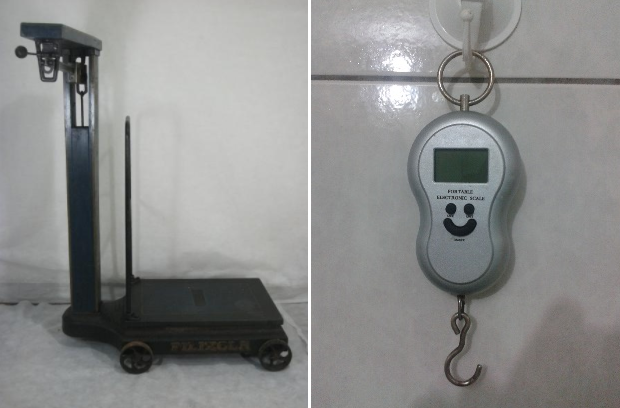
\includegraphics[width=0.7\linewidth]{produtos/prodtres/image021_22}
		\caption{Instrumentos de medição usados na caracterização.}
		\legend{Fonte: Elaborado pelos autores.}
		\label{fig:image021_22}
	\end{figure}


	Para a caracterização dos \gls{rsu}, usou-se de forma adaptada para as características locais, a \gls{nbr} 10004/2004 na classificação e separação por tipo dos resíduos triados, a \gls{nbr} 1007/2004 na amostragem, e o Manual de Gestão dos Resíduos Sólidos do \gls{ibam} para o procedimento de gravimetria.
	
	No processo de caracterização gravimétrica foi observado que o caminhão compactador atualmente destinado ao recolhimento dos resíduos no município coleta aproximadamente 2/3 do que é gerado nas segundas e quartas-feiras, sendo, assim, necessária a complementação da coleta com outro caminhão. Este caminhão tem como função executar somente a coleta seletiva, no entanto, devido a problemas por falta de manutenção na frota, ambas as coletas são feitas pelo mesmo veículo.
	
	\paragraph{\textbf{Metodologia da caracterização gravimétrica:}}
	
	A caracterização dos resíduos da coleta comum foi realizada entre os dias 11 e 16 de dezembro de 2017. Em cada avaliação era utilizado material proveniente da coleta do dia anterior. Após a retirada das lixeiras públicas, o resíduo era transportado para um pátio da \gls{ssm} onde ficava armazenado. O pátio possuía impermeabilização de cimento, porém não havia cobertura. No período da caracterização não houve incidência de chuva.
	
	Foram realizadas 3 amostragens, uma para cada dia de coleta semanal (antigamente realizada às segundas, quartas e sextas-feira). No dia seguinte a coleta, os resíduos armazenados eram espalhados pelo pátio, homogeneizados, quarteados e metade da amostra era removida com auxílio de uma escavadeira. O mesmo processo era aplicado na porção restante. Após, de forma manual, os sacos contendo resíduos eram abertos e o conteúdo novamente espalhado pelo pátio, homogeneizado e, posteriormente espalhados aleatoriamente de forma circular para retirada de 1 m$^{3}$ de resíduos.
	
	Para a pesagem dos resíduos foi utilizado um tambor cilíndrico de plástico de 0,2 m$^{3}$. O preenchimento do tambor foi feito recolhendo resíduos de 5 pontos distintos, percorrendo a circunferência. Sequencialmente, despejou-se novamente o conteúdo do tambor no chão e procedeu-se com a separação dos materiais por tipos e repesagem de cada tipo conforme pode ser observado na \autoref{fig:image22a}.
	
\begin{landscape}
	\begin{figure}
		\centering
		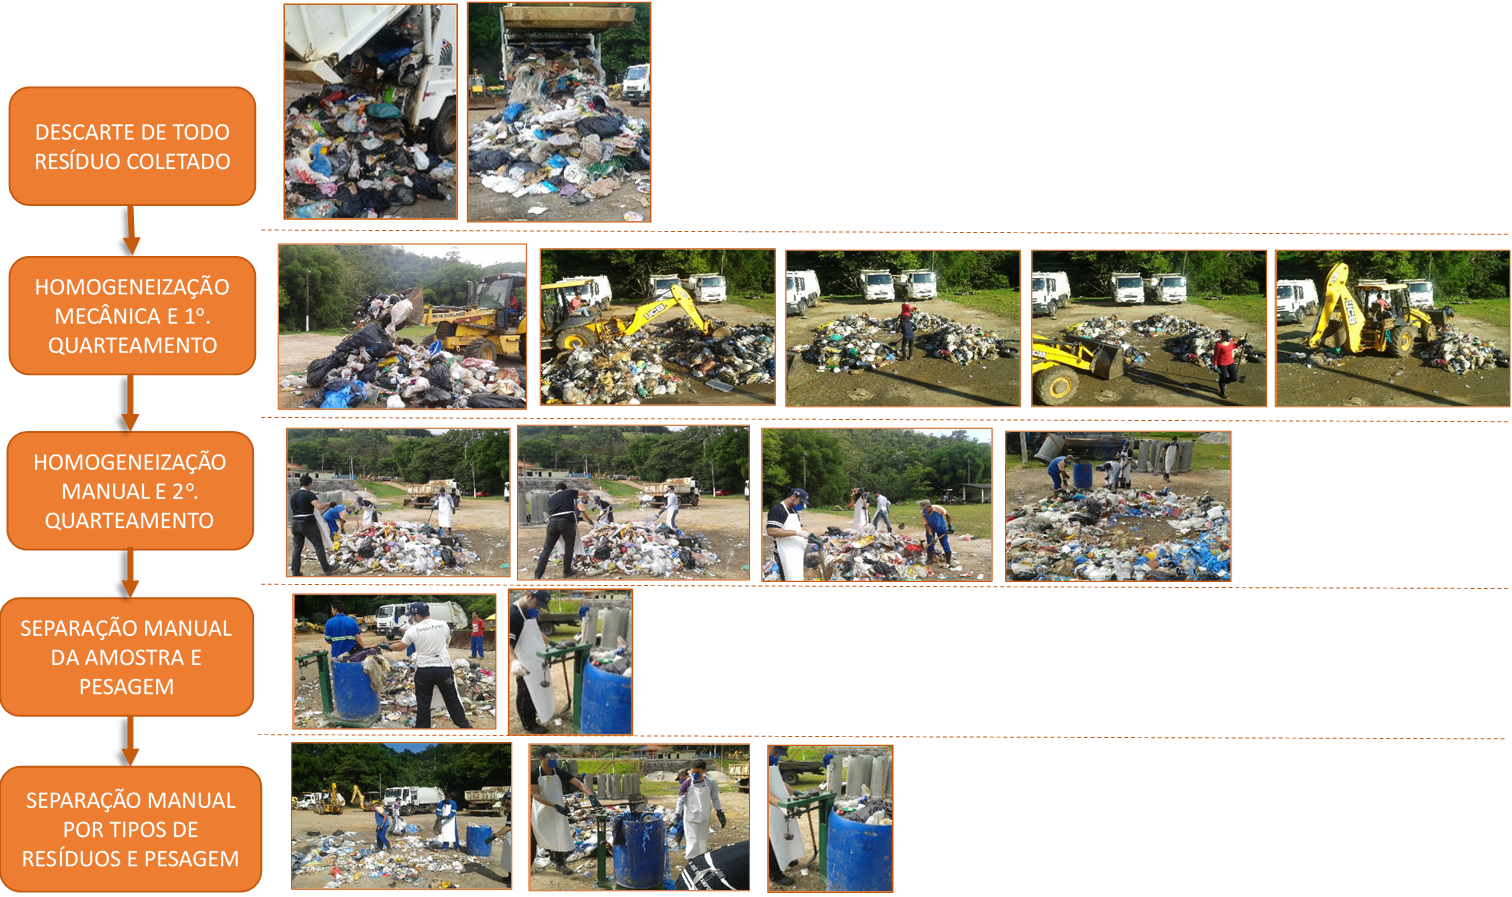
\includegraphics[width=1\linewidth]{produtos/prodtres/image22a}
		\caption{Etapas da caracterização gravimétrica em Monteiro Lobato.}
		\legend{Fonte: Elaborado pelos autores.}
		\label{fig:image22a}
	\end{figure}
\end{landscape}
	
	Devido ao baixo efetivo e à impossibilidade de aferição de resíduos com menor massa, a divisão por tipos de \gls{rsu} se limitou de acordo com a \autoref{tab:tipo_rsu}.
	
	\input{./produtos/prodtres/tipo_rsu}	
	
	\paragraph{\textbf{Resultados da caracterização gravimétrica:}}
	
	Com os dados de cada amostra foi possível obter uma média da composição gravimétrica da coleta comum realizada no município, segundo a \autoref{tab:gravimetrica_comum}. No final de semana antecedente à caracterização gravimétrica, houve uma forte chuva no município, e como os resíduos ficam dispostos nas lixeiras coletivas para posterior coleta, a composição gravimétrica da coleta de segunda-feira pode ter sofrido variação na massa em decorrência do volume de água envolvido juntamente aos resíduos.
	
	\input{./produtos/prodtres/gravimetrica_comum}
	
	Foram obtidas as densidades aparente dos resíduos e sua média referentes aos dias de avaliação, como pode ser observado na \autoref{tab:densidade_aparente}. A densidade média é um valor que pode ser utilizado para o dimensionamento de equipamentos de transporte, instalações de transbordo e tratamento de resíduos sólidos \cite{ibam_manualrs_2001}.

	\input{./produtos/prodtres/densidade_aparente}
	
	A média de geração dos \gls{rsu} comuns referente aos dias de pico avaliados encontra-se ilustrada na \autoref{fig:image039}. O resultado caracteriza-se pelo maior conteúdo de material orgânico, atingindo 34,1 \% do total do \gls{rsu}. Em seguida, com 13 \% e 12,8 \% respectivamente, ocorre a geração de materiais higiênicos e tecidos, sendo em sua maioria roupas ainda em bom estado (\autoref{fig:image040}). 
	
	\begin{figure}
		\centering
		\includegraphics[width=1\linewidth]{produtos/prodtres/image039}
		\caption{Característica da geração de \gls{rsu} da coleta comum (segunda, quarta, sexta)}
		\label{fig:image039}
	\end{figure}
	
	
\begin{figure}
	\centering
	\includegraphics[width=0.7\linewidth]{produtos/prodtres/image040}
	\caption{Tecidos descartados em boas condições de uso.}
	\legend{Fonte: Elaborado pelos autores.}
	\label{fig:image040}
\end{figure}

	Os plásticos como um todo somam 18 \% do \gls{rsu} gerado, sendo 11,4 \% de plástico fino e 6,6 \% de plástico duro; 9,9 \% do total do \gls{rsu} são constituídos de papel e papelão; 5,0 \% são constituídos de metais ferrosos, não ferroso e alumínio; 2,7 \% por madeiras tratadas e não tratadas (naturais); 1,7 \% por pneus; 1,4 \% por vidros coloridos e transparentes; e 1,4 \% por outros materiais que são passíveis de logística reversa e  materiais de \gls{rss} que devem ser acondicionados e armazenados diferenciadamente para posterior tratamento (seringas, medicamentos e embalagens medicamentosas).
	
	Para obtenção de um resultado mais próximo da realidade do município, faz-se necessária outra caracterização em um período de baixa geração ou menor sazonalidade.
	
	\subsection{Resíduos da Coleta Seletiva}
		\label{subsec:res_coleta_seletiva}
	
	Através da obtenção dos dados referentes a geração e coleta de resíduos sólidos recicláveis da plataforma Série Histórica do \gls{snis} para o ano de 2015, a \autoref{tab:coleta_brasil} foi construída \cite{snis_serie_2019_2015}. Analisando a \autoref{tab:coleta_brasil}, observa-se que a taxa de cobertura de coleta seletiva porta-a-porta do país abrange apenas metade da população urbana e que este valor não é homogêneo para cada região.
	
	Enquanto a região Sul possui a maior taxa de coleta seletiva, abrangendo 77 \% da população urbana, as regiões Norte e Nordeste apresentam taxa de coleta seletiva em torno de apenas 15 \%. As regiões Centro-Oeste e Sudeste são as que mais se assemelham a taxa de cobertura do país.
	
	A região Sul se destaca em relação aos outros parâmetros analisados de taxa de material recolhido em relação ao total de resíduos sólidos domésticos (exceto matéria orgânica e rejeitos), massa per capita de materiais recicláveis coletados e massa recuperada em relação a população urbana.
	
	% Table generated by Excel2LaTeX from sheet 'coleta_brasil'
\begin{table}[htbp]
  \centering
  \caption{Informações de coleta e geração de Resíduos Recicláveis no Brasil.}
    \begin{tabular}{c|c|c|c|c}
    \rowcolor[rgb]{ .969,  .588,  .275} \multicolumn{1}{c|}{\textcolor[rgb]{ 1,  1,  1}{\textbf{Região}}} & \multicolumn{1}{P{7.5em}|}{\textcolor[rgb]{ 1,  1,  1}{\textbf{Taxa de cobertura porta-a-porta em relação à população urbana (\%)}}} & \multicolumn{1}{P{7.5em}|}{\textcolor[rgb]{ 1,  1,  1}{\textbf{Taxa de material recolhido em relação à quantidade total coletada de resíduos sól. Domésticos * (\%)}}} & \multicolumn{1}{P{7.5em}|}{\textcolor[rgb]{ 1,  1,  1}{\textbf{Massa per capita de materiais recicláveis recolhidos via coleta seletiva (Kg/hab./ano)}}} & \multicolumn{1}{P{7.5em}}{\textcolor[rgb]{ 1,  1,  1}{\textbf{Massa recuperada per capita de materiais recicláveis em relação à população urbana (Kg/hab./ano)}}} \\
    \rowcolor[rgb]{ .984,  .831,  .706} \multicolumn{1}{c|}{\textbf{Brasil}} & \multicolumn{1}{c|}{\textbf{50,92}} & \multicolumn{1}{c|}{\textbf{6,05}} & \multicolumn{1}{c|}{\textbf{19}} & \textbf{9,39} \\
    \rowcolor[rgb]{ .992,  .914,  .851} \multicolumn{1}{c|}{\textbf{Centro-Oeste}} & \multicolumn{1}{c|}{55} & \multicolumn{1}{c|}{7,18} & \multicolumn{1}{c|}{22} & 10,88 \\
    \rowcolor[rgb]{ .984,  .831,  .706} \multicolumn{1}{c|}{\textbf{Nordeste}} & \multicolumn{1}{c|}{13,68} & \multicolumn{1}{c|}{2,72} & \multicolumn{1}{c|}{9} & 5,02 \\
    \rowcolor[rgb]{ .992,  .914,  .851} \multicolumn{1}{c|}{\textbf{Norte}} & \multicolumn{1}{c|}{15,1} & \multicolumn{1}{c|}{2,41} & \multicolumn{1}{c|}{8} & 12,37 \\
    \rowcolor[rgb]{ .984,  .831,  .706} \multicolumn{1}{c|}{\textbf{Sudeste}} & \multicolumn{1}{c|}{54,31} & \multicolumn{1}{c|}{3,43} & \multicolumn{1}{c|}{13} & 6,17 \\
    \rowcolor[rgb]{ .992,  .914,  .851} \multicolumn{1}{c|}{\textbf{Sul}} & \multicolumn{1}{c|}{77,3} & \multicolumn{1}{c|}{20,38} & \multicolumn{1}{c|}{49} & 21,8 \\
    \rowcolor[rgb]{ .984,  .831,  .706} \multicolumn{5}{c}{\textbf{* exceto matéria orgânica e rejeitos}} \\
    \end{tabular}%
  \label{tab:coleta_brasil}%
  \legend{Fonte  - Adaptado de série histórica SNIS, 2009 a 2015.}
\end{table}%

	
	Os valores da \autoref{tab:coleta_brasil} indicam que, em geral, o Brasil ainda conta com um sistema precário de coleta seletiva e recuperação dos materiais recolhidos. Para melhorar esse panorama, a taxa de cobertura de coleta seletiva deveria ser mais abrangente e, para que o sistema fosse efetivo, seria necessário maior investimento em educação ambiental para que a população fosse mobilizada e sensibilizada a fazer a correta segregação do resíduo domiciliar. Através dessas ações, a taxa de \gls{rsu} destinada a aterros sanitários pode diminuir consideravelmente.
	
	Os dados primários sobre os resíduos recicláveis em Monteiro Lobato foram obtidos por meio de questionário dirigido às \gls{smaa} e \gls{ssm} e avaliação presencial da coleta municipal.
	
	\subsubsection{Acondicionamento}
	
	Os resíduos recicláveis são acondicionados de forma semelhante à dos resíduos sólidos comuns, em sacos plásticos ou em sacolas de supermercados. Da mesma forma, o armazenamento destes resíduos é semelhante ao dos resíduos sólidos comuns, sendo pendurados em portões ou dispostos nas lixeiras de ferro ou de madeira.
	
	Além disso, resíduos maiores como caixas de papelão e isopor costumam ser acondicionados sem nenhuma forma de revestimento nas lixeiras, como apresentado na \autoref{fig:image041_42}.
	
	\begin{figure}
		\centering
		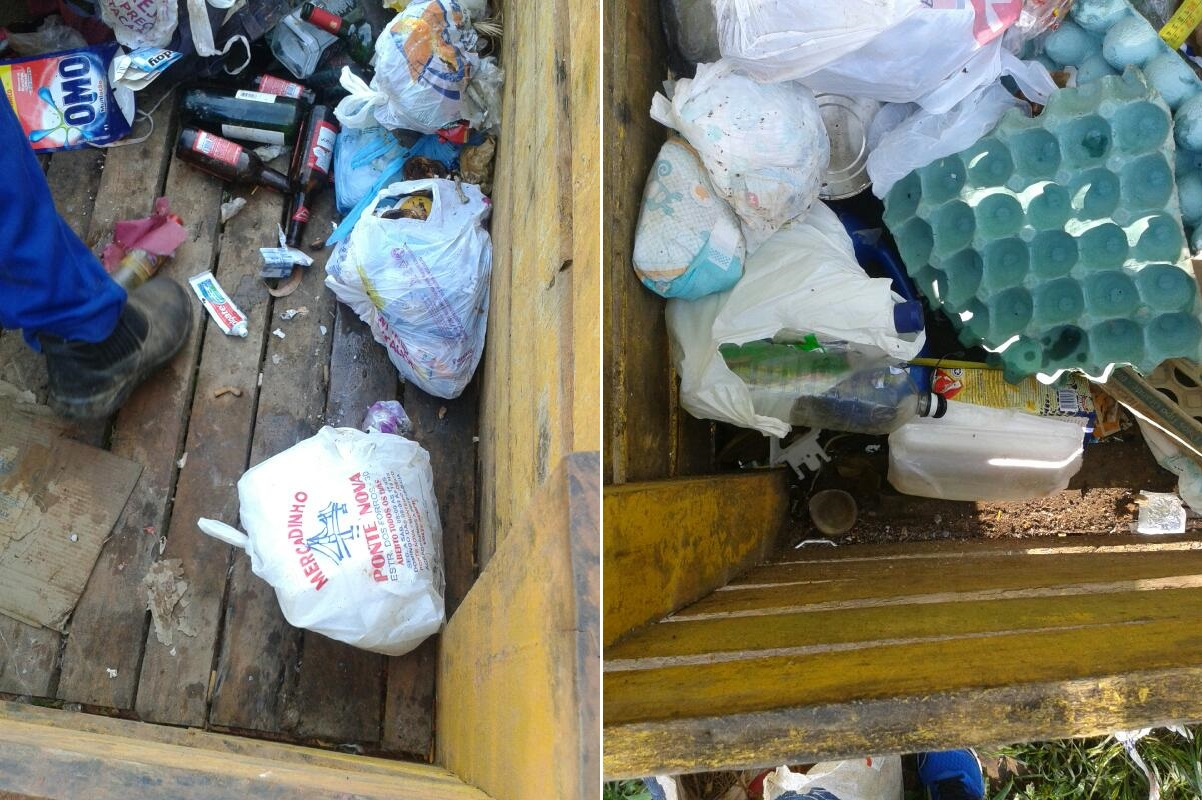
\includegraphics[width=0.7\linewidth]{produtos/prodtres/image041_42}
		\caption{Resíduos recicláveis (garrafas de vidro e de plástico, caixa de papelão, papel) armazenados sem acondicionamento nas lixeiras.}
		\legend{Fonte: Elaborado pelos autores.}
		\label{fig:image041_42}
	\end{figure}
		
	\subsubsection{Coleta, Transbordo e Transporte}
	
	Um problema pelo qual o município passa é em relação ao armazenamento e coleta dos resíduos recicláveis. Atualmente, a coleta do resíduo reciclável ocorre às quartas-feiras em período integral, das 7h às 16h.
	Como o município não dispõe de lixeiras específicas para resíduos comuns e resíduos recicláveis ou de estratégias para diferenciar o acondicionamento, os sacos plásticos de resíduos comuns e recicláveis ficam misturados nas lixeiras e os coletores não são capazes de diferenciar as composições dos sacos no momento da coleta. Deste modo, durante as coletas dos resíduos recicláveis são coletados apenas os resíduos de fácil identificação, como caixas de papelão e garrafas, como exemplificado na \autoref{fig:image043}.
	
	\begin{figure}
		\centering
		\includegraphics[width=0.5\linewidth]{produtos/prodtres/image043}
		\caption{Materiais recicláveis identificáveis por estarem sem acondicionamento nas lixeiras.}
		\legend{Fonte: Elaborado pelos autores.}
		\label{fig:image043}
	\end{figure}
	
	O serviço de coleta de resíduos sólidos recicláveis é realizado pelos mesmos três funcionários responsáveis pela coleta de resíduos comuns. A coleta dos recicláveis ocorre através de um caminhão compactador tipo DMN 2208 com capacidade de 8 m$^{3}$.
		
	Conforme descrição da \gls{ssm}, a coleta de resíduos sólidos recicláveis passa pelas mesmas 59 lixeiras nas quais são armazenados os resíduos sólidos comuns, cujas localizações foram discutidas para o resíduo sólido comum.
	O processo de retirada dos resíduos recicláveis é o mesmo que o realizado para os resíduos sólidos comuns. É feita uma manobra com o caminhão aproximando-o de ré até próximo a lixeira como ilustra a \autoref{fig:image046}. Nesta figura é possível visualizar a dificuldade dos coletores para coleta dos resíduos que não são adequadamente acondicionados.
	
	\begin{figure}
		\centering
		\includegraphics[width=0.7\linewidth]{produtos/prodtres/image046}
		\caption{Retirada dos resíduos recicláveis de lixeira de grande porte.}
		\legend{Fonte: Elaborado pelos autores.}
		\label{fig:image046}
	\end{figure}
	
	
	Como descrito anteriormente, na segunda semana de dezembro de 2017 os percursos de coleta foram acompanhados e as rotas foram registradas através do \gls{gps}. Nesse ano, a coleta seletiva costumava ocorrer às terças e quintas-feiras no período da tarde, ao invés de ser às quartas-feiras como ocorre atualmente. Na \autoref{fig:image047}, é apresentada a rota realizada para a coleta seletiva, referente a uma quinta-feira, mas que pode ser refletida a rota atualmente realizada.
	
	\begin{figure}
		\centering
		\includegraphics[width=1\linewidth]{produtos/prodtres/image047}
		\caption{Rota da coleta de resíduo recicláveis de Monteiro Lobato realizada no período da tarde da quinta-feira.}
		\legend{Fonte: Elaborado pelos autores.}
		\label{fig:image047}
	\end{figure}
	
	
	No período de 2014 a 2018, após o término de toda a coleta, o resíduo era transportado até a \gls{urbam} em São José dos Campos, onde era efetuada a triagem deste material nas instalações do aterro. Assim, a quilometragem percorrida para realização da coleta dos resíduos sólidos recicláveis no município e o transporte de ida e volta resultavam em uma distância média percorrida de 123,3 km (levando em consideração que a distância entre Monteiro Lobato e a \gls{urbam} é de aproximadamente 48 km). A localização da \gls{urbam} em relação ao município é apresentada na \autoref{fig:image048}.
	
	\begin{figure}
		\centering
		\includegraphics[width=1\linewidth]{produtos/prodtres/image048}
		\caption{Localização de Monteiro Lobato e URBAM de São José dos Campos.}
		\legend{Fonte: Elaborado pelos autores.}
		\label{fig:image048}
	\end{figure}
	
	Entretando,  durante a elaboração desse presente produto, o vínculo com a \gls{urbam} foi interrompido e os resíduos recicláveis seguem sem um local de disposição final para onde podem ser transportados.
	
	\subsubsection{Disposição final}
	
	Quando o caminhão chegava à \gls{urbam}, os resíduos eram encaminhados à área de triagem. Após a deposição do material na área de triagem da \gls{urbam}, os resíduos passavam por uma esteira rotativa sendo separados manualmente por catação, do início ao fim do processo. Os materiais selecionados e separados eram enfardados para então serem comercializados, enquanto os materiais descartados na triagem, eram destinados a área de aterramento onde recebiam sua disposição final. 
	
	De uma forma geral, o sistema de coleta de resíduos seletivos, para o período de 2014 a 2018, podia ser esquematizado conforme a \autoref{fig:image017b}.
	
	\begin{figure}
	\centering
	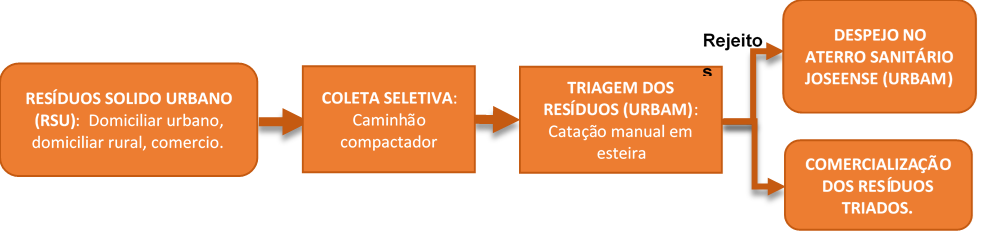
\includegraphics[width=1\linewidth]{produtos/prodtres/image017b}
	\caption{Gerenciamento dos resíduos seletivos por Monteiro Lobato.}
	\legend{Fonte: Elaborado pelos autores.}
	\label{fig:image017b}
	\end{figure}

	Conforme supracitado, os resíduos recicláveis encontram-se atualmente, no ano de 2019 sem local fixamente pré-definido por contrato. Dessa forma, os resíduos recicláveis são levados a um outro local de disposição de modo informal, podendo ocorrer ou não o correto encaminhamento do material.
	
	\subsubsection{Volume gerado}
	
	Através de dados disponibilizados pela \gls{ssm}, dos valores totais mensais e a quantidade de coletas realizadas dos meses de março a outubro de 2017, foi possível realizar algumas análises sobre a dinâmica e atuação do município para com os resíduos recicláveis. A avaliação dessas informações permite que sejam compreendidos a dinâmica de geração de resíduos recicláveis e os hábitos de segregação entre resíduos recicláveis e comuns e auxilia no desenvolvimento de diretrizes e ações que visem a melhoria do gerenciamento dos resíduos recicláveis.
	
	Com base nos dados fornecidos e projeções populacionais do \gls{ibge} foi possível estimar a geração per capita diária de resíduos sólidos recicláveis entre março e outubro de 2017 (vide \autoref{fig:image049}). Percebe-se uma tendência entre os meses de março e agosto, que apresentam valor per capita diário de aproximadamente 0,04 kg por habitante por dia. Para os meses de setembro e outubro é observada uma queda brusca na geração.
	
	\begin{figure}
		\centering
		\includegraphics[width=0.75\linewidth]{produtos/prodtres/image049}
		\caption{Geração per capita de resíduo sólido reciclável de Monteiro Lobato.}
		\label{fig:image049}
	\end{figure}
	
	
	Com a estimativa desses dados é possível verificar que o potencial de reciclagem do município é muito baixo. Considerando que a geração per capita de resíduo sólido domiciliar de Monteiro Lobato é a soma entre a geração per capita diária de resíduo comum e a geração per capita diária de resíduo reciclável, a geração per capita de resíduo reciclável representa, aproximadamente, 8 \% da geração per capita total.
	Na coleta dos \gls{rsu} seletivos, recolhe-se todo o resíduo gerado pela população durante uma semana anterior. Um problema recorrente no município é a ausência de lixeiras separadas para resíduos recicláveis, o que pode acarretar em uma diferença na quantidade de resíduos recicláveis coletados para a quantidade real de resíduos colocados nas lixeiras além de haver dificuldade na diferenciação dos sacos de resíduos recicláveis dos comuns pelos coletores.
	
	\subsubsection{Caracterização gravimétrica}
	
	\paragraph{\textbf{Metodologia da caracterização gravimétrica}}
	

	A caracterização gravimétrica e a avaliação dos \gls{rsu} seletivos ocorreram igualmente ao processo descrito para a metodologia dos resíduos sólidos comuns \ref{subsubsec:gravimetria_comum}. Para os resíduos provenientes da coleta seletiva foram realizadas 2 amostragens dos seus respectivos dias de coleta semanal (terça e quinta-feira, dias antigos de coleta reciclável referente à data em que essa caracterização foi realizada, em 2017). Devido ao baixo efetivo e à impossibilidade de aferição de resíduos com menor massa, a divisão por tipos de resíduos se limitou à disposta na \autoref{tab:tipo_rsu_ml}. Não houveram alterações nas condições climáticas que comprometessem a caracterização desses resíduos.

	
	\input{./produtos/prodtres/tipo_rsu_ml}
	
	\paragraph{\textbf{Resultados da caracterização gravimétrica}}
	
	Com os dados de cada amostra foi possível obter uma média da composição gravimétrica da coleta comum realizada no município, conforme a \autoref{tab:gravimetrica_seletiva}.
	
	\input{./produtos/prodtres/gravimetrica_seletiva}
	
	Medindo-se as amostras obteve-se as densidades aparentes dos resíduos da coleta seletiva referentes aos dias de avaliação, bem como a média como pode ser observado na \autoref{tab:densidade_aparente_seletiva}.
	
	\input{./produtos/prodtres/densidade_aparente_seletiva}
	
	A característica dos \gls{rsu} seletivos (\autoref{fig:image050}) no período de maior geração no município é de 40,5 \% de papelão como material presente em maior quantidade seguido de plásticos totalizando 25,1 \% sendo que desses, 14,4 \% são plásticos duros e 10,7 \% são plásticos finos. Vidros coloridos e transparentes contribuem com 19,4 \% e papeis representam 3,8 \%, seguidos pelos materiais que são passíveis de logística reversa (embalagens de óleos automotivos, lâmpadas fluorescentes, equipamento eletroeletrônicos e pilhas) e materiais de \gls{rss} (seringas, medicamentos e embalagens medicamentosas), que devem ser acondicionados e armazenados diferenciadamente para posterior tratamento, constituindo estas classes 2,4 \% do total. 
	
	Na caracterização gravimétrica também foi catalogada a presença de materiais higiênicos (2,3 \%) e materiais orgânicos (2,1 \%), os quais contaminam materiais recicláveis, podendo reduzir ou até inviabilizar a reciclagem desses materiais com tal potencial. Em menor proporção ocorreram embalagens Tetra Pak com 1,3 \%, metais diversos 1,1 \%, isopor 0,5 \% e tecido 1,4 \% conforme demonstra a \autoref{fig:image050}.
	
	\begin{figure}
		\centering
		\includegraphics[width=0.75\linewidth]{produtos/prodtres/image050}
		\caption{Característica da geração de resíduos da coleta seletiva (terça e quinta).}
		\legend{Fonte: Elaborado pelos autores.}
		\label{fig:image050}
	\end{figure}

	
	Para um resultado mais próximo da realidade do município, faz-se necessária outra caracterização em um período de baixa geração ou menor sazonalidade.
	
	\subsection{Resíduos de Limpeza Urbana}
	
	Os resíduos sólidos do serviço de limpeza urbana englobam os oriundos de varrição, limpeza de logradouros e vias públicas, poda de árvores, capina e roçagem, limpeza de feiras, limpeza de praias, limpeza da rede de drenagem, limpeza de bocas de lobo e desobstrução de ramais \cite{brasil:12305, brasil:11445, ibam_manualrs_2001} e o seu manejo objetivam manter as condições de higiene dos logradouros e a boa qualidade dos sistemas de drenagem de águas pluviais evitando assim problemas de saúde de caráter sanitário e inundações nas regiões urbanas. Os serviços de limpeza urbana também evitam a geração de maus cheiros oriundos da decomposição de matéria orgânica de frutos ou de materiais provenientes de feiras. Em Monteiro Lobato são realizadas as atividades de varrição das vias públicas, poda e capina, limpeza de sistema de drenagem pluvial, limpeza de cemitério e de feira livre.
	
	De acordo com o artigo 7 da Lei nº 11.445 de 2007, o serviço público de limpeza urbana deve se responsabilizar pela coleta, transbordo e transporte dos resíduos; pela respectiva triagem para fins de reuso ou reciclagem; pelo tratamento, inclusive por compostagem, e disposição final dos resíduos originários dos serviços de limpeza urbana descritos anteriormente \cite{brasil:11445}. Uma boa atuação da Prefeitura nesse sentido pode refletir nas atitudes dos munícipes incentivando a correta destinação e desenvolver o grau de educação ambiental. Além disso, uma satisfatória limpeza urbana promove uma estética agradável para a cidade, o que é vantajoso para Monteiro Lobato pois se trata de um município que investe no desenvolvimento turístico.
	 
	As informações sobre manejo da limpeza urbana, custos associados, equipamentos utilizados, responsabilidades dos funcionários e horários da realização dos serviços foram obtidas através de questionário estruturado encaminhado em forma de ofício à \gls{ssm} e \gls{smaa}. De acordo com as respostas, além da quantidade específica de funcionários para atividades de varrição e poda e capina, existem sete funcionários (cinco de frente de trabalho, um da \gls{smaa} e um da \gls{ssm}) que colaboram com as demais atividades referentes à limpeza urbana, quando necessário.
	
	O serviço de varrição em Monteiro Lobato ocorre todos os dias da semana, das 07h às 11h e das 12h às 16h. Entre segunda e sexta-feira são efetuadas a limpezas nas praças e logradouros da região central, rodoviária e nos bairros Jardim Iracema, Vila São Sebastião, Jardim Morada do Sol, Vila Esperança, Souza e São Sebastião. Aos finais de semana a limpeza fica limitada ao serviço a região central e rodoviária no período da manhã.
	
	Durante o serviço de varrição, ocasionalmente os sacos plásticos de 60 litros das lixeiras públicas são retirados, colocados no carrinho de mão, encaminhados e armazenados no pátio da \gls{ssm} para posteriormente serem coletados pelo caminhão da coleta comum.
	

	Para a varrição, o município dispõe de cinco funcionários contratados pela prefeitura e de, normalmente, cinco funcionários da frente de trabalho, que colaboram com o serviço. Para a varrição, são utilizadas vassouras, pás de lixo e carrinho de lixo de capacidade de 240 litros (vide \autoref{fig:image051}), sendo que cada funcionário percorre em média 3 km por dia.

	\begin{figure}
		\centering
		\includegraphics[width=0.7\linewidth]{produtos/prodtres/image051}
		\caption{Funcionários com equipamentos de serviço de varrição.}
		\legend{Fonte: \gls{ssm} de Monteiro Lobato.}
		\label{fig:image051}
	\end{figure}
	
	Outro serviço de limpeza urbana prestado pelo município é o de poda e capina e que ocorre de duas formas distintas. Às sextas-feiras ocorrem as podas, conforme pedido efetuado pelo munícipe à Central do Cidadão. Já de segunda a sexta-feira ocorre a capina conforme cronograma da \gls{ssm}. A tarefa é normalmente realizada por quatro funcionários. Os equipamentos utilizados para poda e capina são a enxada, enxadão, pá, motosserra, foice, machado, serra manual e caminhão basculante com capacidade para 5 metros cúbicos.

	Em Monteiro Lobato é realizada uma feira semanalmente aos sábados, das 9 horas às 14 horas, onde comercializa-se principalmente produtos alimentícios da própria região. A feira é de pequeno porte e seus resíduos gerados são acondicionados nas lixeiras públicas pelos próprios munícipes. Semanalmente, ocorre a limpeza do cemitério municipal que produz como resíduo, em sua maioria, flores, vasos e grãos provenientes da varrição (\autoref{fig:image052}). Este serviço é conduzido por um funcionário.
	
	\begin{figure}
		\centering
		\includegraphics[width=0.5\linewidth]{produtos/prodtres/image052}
		\caption{Exemplos de resíduos cemiteriais.}
		\legend{Fonte: \gls{ssm} de Monteiro Lobato.}
		\label{fig:image052}
	\end{figure}

	
	Os resíduos da rede de drenagem são provenientes da limpeza de bocas de lobo, sarjeta e bueiros, de onde se retiram os sedimentos como areia e argila e resíduos sólidos que se depositam nestes locais prejudicando a drenagem das águas pluviais. Essa limpeza ocorre semanalmente e quando há solicitação pelos moradores através da Central do Cidadão. O trabalho usualmente é realizado normalmente por quatro funcionários, através de enxadas, pás e carrinho de mão de capacidade de 60 litros, sendo três funcionários para limpeza e um motorista.
	
	\subsubsection{Acondicionamento}
	
	Após as varrições, os resíduos acumulados são acondicionados em sacos plásticos e encaminhados e armazenados na garagem da \gls{ssm}.  Já os resíduos provenientes do serviço de poda e capina são armazenados no pátio da Prefeitura localizado no Bairro Morada do Sol, apresentado na \autoref{fig:image053}, até serem coletados e destinados. Os resíduos oriundos do serviço de limpeza da rede de drenagem são acondicionados em carrinhos de mão e são também armazenados no pátio do bairro Morada do Sol até coleta.

	
	\begin{figure}
		\centering
		\includegraphics[width=0.75\linewidth]{produtos/prodtres/image053}
		\caption{Pátio do bairro Morada do Sol onde é acondicionado parte dos resíduos de poda e capina.}
		\legend{Fonte: Fornecida pela \gls{ssm}.}
		\label{fig:image053}
	\end{figure}
		
	Os resíduos gerados pela feira livre do município são coletados pelos próprios usuários da feira e são acondicionados em sacos pretos de 200 litros dentro das lixeiras públicas, como as da \autoref{fig:image054}, localizadas próximas aos mercados da praça.

	\begin{figure}
		\centering
		\includegraphics[width=0.7\linewidth]{produtos/prodtres/image054}
		\caption{Lixeiras públicas localizadas na praça de Monteiro Lobato.}
		\legend{Fonte: Fornecida pela \gls{ssm}.}
		\label{fig:image054}
	\end{figure}
	
	
	Os resíduos do cemitério são acondicionados em sacos plásticos de 200 litros e mantidos no próprio cemitério até que seja realizada a coleta.
	
	\subsubsection{Coleta, Transbordo e Transporte}
	
	Após os respectivos acondicionamentos dos resíduos sólidos oriundos da limpeza urbana, todos sacos plásticos são coletados pelo caminhão responsável pela coleta comum do município e seguem para o mesmo destino dos resíduos sólidos domiciliares, o aterro sanitário de Tremembé ESTRE-Resicontrol.
	
	\subsubsection{Disposição final}
	O material proveniente do serviço de poda e capina, atualmente, é encaminhado para o pátio do \gls{cdm} no bairro Morada do Sol. Neste local ocorre a compostagem aeróbica para transformação do material orgânico em composto, que é usado em atividade de jardinagem. Como esse procedimento é novo no município, não se tem a quantidade de material encaminhado e transformado neste local. 
	A disposição final dos resíduos oriundos do serviço de varrição, limpeza de rede de drenagem, feiras e do cemitério é realizada em conjunto com os resíduos sólidos comuns do município de Monteiro Lobato, no aterro sanitário ESTRE-Resicontrol.
	
	\subsubsection{Volume}
	
	O município não possui um controle da quantidade gerada em volume ou em peso dos resíduos oriundos dos serviços de limpeza urbana de varrição, poda e capina, limpeza do cemitério, limpeza da feira e limpeza da rede de drenagem.
	Apesar de se conhecer o volume dos sacos plásticos onde os resíduos são acondicionados, não há o controle da quantidade de sacos plásticos que costumam ser retirados para cada atividade ou se os mesmos são preenchidos até a sua capacidade total.
	
	\subsubsection{Custos}
	
	Como o município não possui renda específica para gerenciamento dos resíduos sólidos e a manutenção dos equipamentos do serviço de limpeza urbana não é frequente não há um controle sobre o custo associado a esse serviço. No entanto, é possível estimar o custo relacionados aos funcionários para cada atividade considerando o valor médio de salário base somado aos descontos e \gls{fgts} calculado através dos dados disponibilizados pela \gls{ssm} e pela quantidade de funcionários responsáveis por cada serviço. A estimativa do gasto da Prefeitura com os serviços de limpeza urbana engloba também o valor destinado aos cinco funcionários de frente de trabalho que colaboram com a manutenção e atividades em alguns serviços, ajudando principalmente na varrição.  A \autoref{tab:custo_slu} apresenta os gastos aproximados com os funcionários para cada atividade de limpeza urbana, obtidos em 2017.
	
	\input{./produtos/prodtres/custo_slu}
	
	\subsection{Resíduos dos Serviços Públicos de Saneamento Básico}
	
	Resíduos de serviços públicos e saneamento básico são aqueles englobados por um conjunto de serviços, infraestruturas e instalações operacionais de: abastecimento de água potável, esgotamento sanitário, limpeza urbana e manejo de resíduos sólidos e drenagem e manejo das águas pluviais, limpeza de vias públicas e logradouros, limpeza e fiscalização preventiva das respectivas redes urbanas \cite{brasil:12305}.  
	
	As redes de drenagem urbana tradicionalmente são compostas por dois subsistemas: o sistema inicial de drenagem e o sistema de macrodrenagem. O primeiro é composto pelos pavimentos das ruas, guias e sarjetas, bocas de lobo, rede de galerias de águas pluviais e canais de pequenas dimensões. Esse sistema, quando bem planejado e mantido, contém as enxurradas e inundações, evitando problemas nas atividades urbanas. O sistema de macrodrenagem é composto por canais, abertos ou de contorno fechado, de dimensões maiores que os do sistema inicial de drenagem \cite{sp_drenagem_1999}.
	
	As redes de drenagem urbana são uma fonte de poluição difusa e principal fato degradante de rios, lagos e estuários pois veiculam uma grande e diversa carga de poluentes provenientes da disposição incorreta dos mesmos na superfície \cite{brites_drenagem_2004}. Na rede de microdrenagem do município de Monteiro Lobato são lançados materiais de diversos tipos, obstruindo a passagem das águas pluviais e assim tornando-se um fator favorável às inundações e alagamentos \cite{ml_pmisb_2007}.
 	
	Os titulares dos serviços públicos de saneamento básico poderão delegar a organização, regulação, a fiscalização e a prestação desses serviços. Cabe ao titular formular a política pública de saneamento básico através da elaboração de planos de saneamento básico, dentre outras atividades previstas na Lei nº 11.445 de 2007.
	
	É de competência do Estado de São Paulo o planejamento, fiscalização, regulação dos serviços municipais de abastecimento de água e esgotamento sanitário no município. Já a limpeza, desobstrução e recolhimento de detritos formados nas bocas de lobo, que compõem a rede de microdrenagem do município são de responsabilidade do município. O serviço é realizado semanalmente pela \gls{ssm} ou quando solicitado por munícipes através de requerimento via Central do Cidadão.
	
	No município de Monteiro Lobato, a Lei 1.378 de 10 de outubro de 2007 autoriza a \gls{sabesp} a realizar os serviços municipais de abastecimento de água e esgotamento sanitário. Esses serviços abrangem, no todo ou em parte, as atividades de captação, adução e tratamento de água bruta; a adução, reserva e distribuição de água tratada; e a coleta, transporte, tratamento e disposição final de esgotos sanitários \cite{ml_pmisb_2007}.

	Neste contexto, os lodos gerados das \gls{eta} e \gls{ete} são classificados como resíduos sólidos pela norma da \gls{abnt} \gls{nbr} 10004:2004 e podem ser englobados como resíduos de serviços públicos e saneamento básico \cite{sp_pers_2014}.
	
	\paragraph{\textbf{Sistema de \gls{eta} em Monteiro Lobato}}
	
	O município é composto por três sistemas de abastecimento de água: O principal, que é denominado Sistema Sede, e os isolados, determinados de Reservatório São Benedito e \gls{eta} Jair Dimas, no bairro do Souzas, apresentados nas Figuras \ref{fig:image055}, \ref{fig:image056} e \ref{fig:image057}. 
	
	\begin{figure}
		\centering
		\includegraphics[width=0.75\linewidth]{produtos/prodtres/image055}
		\caption{Sistema Sede – Estação de Tratamento de Água de Monteiro Lobado.}
		\legend{Fonte: Elaborado pelos autores.}
		\label{fig:image055}
	\end{figure}

	
	\begin{figure}
		\centering
		\includegraphics[width=0.75\linewidth]{produtos/prodtres/image056}
		\caption{Reservatório de Água do bairro São Benedito.}
		\legend{Fonte: Elaborado pelos autores.}
		\label{fig:image056}
	\end{figure}
	
	
	\begin{figure}
		\centering
		\includegraphics[width=0.75\linewidth]{produtos/prodtres/image057}
		\caption{ETA Jair Dimas Moreira - Bairro do Souzas.}
		\legend{Fonte: Elaborado pelos autores.}
		\label{fig:image057}
	\end{figure}
	
	
	Em 2007 estes sistemas atendiam 99\% da área urbana %\cite{ml_pmisb_2007}. 
	Atualmente, de acordo com a \gls{sabesp}, a \gls{eta} Sede trata 10.686 m$^{3}$ de água por mês e a \gls{eta} do Bairro do Souzas, trata um volume mensal de 1.795 m$^{3}$. Não foi informado o volume de água tratada por mês pelo Reservatório São Benedito, que recebe a água do poço. Como a água do poço contém ferro e manganês, esta água passa por um filtro. Atualmente este filtro é limpado diariamente e os resíduos retirados são descartados diretamente no corpo receptor ao redor.
	
	\paragraph{\textbf{Sistema de \gls{ete} em Monteiro Lobato}}
	
	O sistema de esgotamento sanitário do município de Monteiro Lobato abrange a área urbana do município e contempla de 4 estações, sendo elas: Sistema Sede, \gls{ete} Jardim Iracema, \gls{ete} Souzas e ETE São Benedito. Em 2007, apresentava um índice de coleta de 73 \% e tratamento de 88 \% desse esgoto coletado. 

	O Sistema Sede possui uma e capacidade nominal de 6 l/s trata 5,6 l/s de esgoto da área urbana e o efluente final tratado é lançado no Rio Buquira. A \gls{ete} Jardim Iracema se encontrava em reforma durante o levantamento dos dados e não foi possível realizar a visita. 
	
	O Sistema da \gls{ete} do Bairro dos Souzas na \autoref{fig:image058}, possui apenas um sistema coletor isolado, contempla 50 \% do bairro e lança o esgoto in natura no Córrego Faria \cite{ml_pmisb_2007}. 
	
	\begin{figure}
		\centering
		\includegraphics[width=0.75\linewidth]{produtos/prodtres/image058}
		\caption{ETE Bairro Souzas.}
		\legend{Fonte: Elaborado pelos autores.}
		\label{fig:image058}
	\end{figure}
	
	
	A \gls{ete} São Benedito trata o esgoto que é recebido de uma Estação Elevatório, como mostra, respectivamente, na \autoref{fig:image059}. 
	
	\begin{figure}
		\centering
		\includegraphics[width=0.75\linewidth]{produtos/prodtres/image059}
		\caption{ETE e Elevatório em São benedito.}
		\legend{Fonte: Elaborado pelos autores.}
		\label{fig:image059}
	\end{figure}
	
	
	Tanto a \gls{ete} São Benedito quanto a \gls{ete} do Bairro do Souzas apresentam um sistema preliminar composto por gradeamento e desarenador, como apresentado na \autoref{fig:image060}. Os sólidos grosseiros retidos nas grades são retirados periodicamente, acondicionados em baldes e levados para o Sistema Sede, onde são acondicionados em tanques juntamente com os resíduos provenientes dos filtros. Estes resíduos são coletados por empresa terceirizada.
	
	\begin{figure}
		\centering
		\includegraphics[width=0.25\linewidth]{produtos/prodtres/image060}
		\caption{Sistema de gradeamento seguido de desarenador.}
		\legend{Fonte: Elaborado pelos autores.}
		\label{fig:image060}
	\end{figure}
	
	
	\subsubsection{Disposição final}
	
	A empresa responsável pela coleta do lodo e do resíduo gerado na etapa de gradeamento no Sistema de Tratamento de Esgoto é a Essencis Ecossistema Ltda, que atua, nesse serviço, desde 2010 no município. Além disso, a empresa é responsável por coletar os resíduos oriundos dos desarenadores e os resíduos retidos no Elevatório São Benedito (vide \autoref{fig:image061}). 
	
	\begin{figure}
		\centering
		\includegraphics[width=0.25\linewidth]{produtos/prodtres/image061}
		\caption{Poço do Sistema Elevatório São Benedito que recebe o Esgoto e possui os resíduos coletados por empresa terceirizada periodicamente.}
		\legend{Fonte: Elaborado pelos autores.}
		\label{fig:image061}
	\end{figure}
	
	
	A coleta dos resíduos procedentes das \gls{eta} e \gls{ete} ocorre bimestralmente. A coleta da empresa abrange todas as subestações, com exceção do Reservatório São Benedito e da \gls{eta} do Bairro do Souzas, que atualmente também descartam o lodo gerado em corpo receptor, mas tem previsões de instalar um tratamento ou leito de secagem.
	
	Segundo a \gls{sabesp}, atualmente, o lodo coletado no município é levado para a \gls{ete} Jardim Iracema onde ocorre o processo de tratamento e o lodo ativado é disposto em leito de secagem. Passado o tempo necessário, o lodo é acondicionado em caçambas para ser feita a destinação final.
	
	Assim, tanto o lodo gerado no tratamento do esgoto sanitário quanto os resíduos provenientes do gradeamento das estações são destinados ao aterro sanitário certificado para sua disposição final, de acordo com informações concedidas pela \gls{sabesp}. 
	
	\subsubsection{Volume}
	De acordo com informações levantadas pela \gls{sabesp}, a \gls{ete} Jardim Iracema com seu processo de tratamento do esgoto sanitário tem uma geração de lodo seco desidratado de 10 toneladas por ano.
	
	\subsection{Resíduos Industriais}
	\label{sub_ri}
	
	Os resíduos industriais são aqueles gerados nos processos produtivos e de instalações industriais cujas particularidades tornem inviável o seu lançamento na rede pública de esgoto ou em corpos d’água, ou exijam, para isso, soluções técnica ou economicamente inviáveis \cite{brasil:12305, conama:313}. Podem ser originados dos mais diversos ramos industriais, como metalúrgico, químico, petroquímico, alimentício, mineração, entre outros.  %\cite{IPEA2012b}.
	
	Devido às diferentes possibilidades de origem, os resíduos industriais podem ser compostos por resíduos perigosos ou não perigosos \cite{conama:313}. Os resíduos industriais abrangem resíduos de processo, resíduos de operação de controle de poluição ou descontaminação, resíduos da purificação de matérias-primas e produtos, cinzas, lodos, óleos, resíduos alcalinos, resíduos ácidos e até mesmo resíduos plásticos, papel, madeira, fibras, borracha, metal, escórias, vidros e cerâmicas. %\cite{IPEA2012b}.
	
	No Brasil há 4 unidades de aterros industriais cadastradas, sendo 3 da região sudeste e 1 da região sul. Dessas, 1 é operada por instituição pública e 3 por empresas privadas. A massa total de resíduos recebidos por essas unidades de processamento é de 5.793 toneladas \cite{snis_serie_2016}.
	
	Em escala estadual, foi previsto um aumento da geração de resíduos industriais de cerca de 95,8 milhões de t/ano, em 2010, para próximo de 190,7 milhões t/ano em 2030. A \autoref{tab:evolucao_ri} mostra a tendência de crescimento na geração dos resíduos industriais entre 2010 e 2030 \cite{sp_pers_2014}.
	
	\input{./produtos/prodtres/evolucao_ri}
	
	O município de Monteiro Lobato tem apenas uma planta industrial, denominada “Água Mineral Natural Monteiro Lobato da Mineração Monteiro Lobato Ltda”. Através de visita à essa planta em conjunto com a \gls{smaa} (vide \autoref{fig:image062}), foi verificado que a planta apresenta Plano de Gerenciamento de Resíduos Sólidos, segue os regulamentos do \gls{dnpm}, está devidamente licenciada para operação com a \gls{cetesb} e regularizada com o Cadastro Técnico Federal de Regularidade do \gls{ibama}.
	
	\begin{figure}
		\centering
		\includegraphics[width=0.75\linewidth]{produtos/prodtres/image062}
		\caption{Visita técnica à Mineração Monteiro Lobato Ltda.}
		\legend{Fonte: Elaborado pelos autores.}
		\label{fig:image062}
	\end{figure}
	
	
	\subsubsection{Diretrizes iniciais para elaboração do Plano de Gerenciamento de Resíduos Sólidos Industriais}
	
	Considerando os princípios da gestão integrada e compartilhada da \gls{pnrs}, e de acordo com Plano de Resíduos Sólidos do Estado de São Paulo são atribuídas as seguintes responsabilidades aos geradores de resíduos industriais:
	
	\begin{itemize}
		\item o gerenciamento desde a geração até a disposição final do resíduo sólido e elaboração de Plano de Gerenciamento de Resíduos Sólidos.
		\item para geradores de resíduos industriais perigosos - o gerenciamento, mesmo que tratados, reciclados ou recuperados para utilização como adubo, matéria prima ou fonte de energia, bem como no caso de duas incorporações em materiais, substâncias ou produtos (dependerá de prévia aprovação dos órgãos competentes) e elaboração de Plano de Gerenciamento de Resíduos Sólidos.
	\end{itemize}

	De acordo com o Art. 13 da \gls{pnrs}, os resíduos industriais caracterizados como não perigosos podem ser considerados similares aos resíduos domiciliares diante de sua natureza e composição pelo poder público municipal. No entanto, o plano de gerenciamento de resíduos sólidos industriais deve ser elaborado pelo gerador independentemente da composição do resíduo gerado \cite{brasil:12305}.

	Além de seguir a ordem de prioridade de não geração, redução, reutilização, reciclagem, tratamento e destinação final, de acordo com o Art. 21 da \gls{pnrs}, o conteúdo mínimo que um plano de gerenciamento de resíduos sólidos deve apresentar engloba \cite{brasil:12305}:
	
	\begin{enumerate}[label=\Roman*]
%o uso do parênteses na atribuição do rótulo coloca a numeração da	lista entre parênteses. Se não usado, não exibe parênteses		
		\item Descrição do empreendimento ou atividade;
		\item Diagnóstico dos resíduos sólidos gerados ou administrados contemplando a origem, o volume e a caracterização dos resíduos, incluindo os passivos ambientais a eles relacionados;
		\item Observadas as normas estabelecidas pelos órgãos do \gls{sisnama}, do \gls{snvs}, do \gls{suasa} e, se houver, o plano municipal de gestão integrada de resíduos sólidos:
		\begin{enumerate}[label=(\alph*)] 
			\item Explicitação dos responsáveis de cada etapa do gerenciamento de resíduos sólidos;
			\item Definição dos procedimentos operacionais relativos às respectivas etapas do gerenciamento de resíduos sólidos;
		\end{enumerate}
		\item Identificação das soluções consorciadas ou compartilhadas com outros geradores;
		\item Ações preventivas e corretivas a serem executadas em situações de gerenciamento inadequado ou acidentes;
		\item Metas e procedimentos relacionados à minimização da geração de resíduos sólidos e, de acordo com as normas estabelecidas pelos órgãos do \gls{sisnama}, do \gls{snvs} e do \gls{suasa}, à reutilização e reciclagem;
		\item Ações relativas à responsabilidade compartilhada pelo ciclo de vida dos produtos, na forma do artigo 31 da \gls{pnrs}, se couber;
		\item Medidas saneadoras dos passivos ambientais relacionados aos resíduos sólidos gerados;
		\item Periodicidade de sua revisão, considerando, se couber, o prazo de vigência da respectiva licença de operação a cargo dos órgãos do \gls{sisnama}.
	\end{enumerate}

	Vale ressaltar que a elaboração e aplicação do plano de gerenciamento de resíduos sólidos não é afetada ou impedida diante da ausência do \gls{pmgirs} \cite{brasil:12305}.

	\subsubsection{Inventário de Resíduos Sólidos Industriais}
	
	O Inventário Nacional de Resíduos Sólidos Industriais, instrumento da \gls{pnrs}, apresenta informações sobre geração, armazenamento, transporte, tratamento, reutilização, reciclagem, recuperação e disposição final destes resíduos. 
	
	Para alguns setores estas informações deveriam ser apresentadas até o ano de 2003, sendo eles: indústrias de preparação de couros e fabricação de artefatos de couro; fabricação de coque, refino de petróleo, elaboração de combustíveis nucleares e produção de álcool; fabricação de produtos químicos; metalurgia básica; fabricação de produtos de metal; fabricação de máquinas e equipamentos, máquinas e equipamentos, máquinas para escritório e equipamentos de informática; fabricação e montagem de veículos automotores, reboques e carrocerias; e fabricação de outros equipamentos de transporte. Essas informações devem ser atualizadas a cada dois anos \cite{conama:313}.
	
	Apesar da obrigatoriedade, não foi identificado o Inventário de Resíduos Sólidos Industriais do estado de São Paulo. Esse fato intensifica a necessidade da elaboração de planos de gerenciamento de resíduos industriais e da devida fiscalização pelo órgão ambiental responsável para que os \gls{ri} do estado detenham disposição final ambientalmente adequada.
	
	As normas constituem uma ferramenta importante para a correta classificação de resíduos industriais e gerenciamento dos mesmos. Estas são listadas na \autoref{tab:nbr_ri}.
	
	\input{./produtos/prodtres/nbr_ri}
	
	\subsubsection{Volume}
	De acordo com as atividades da planta industrial, a geração de resíduos se dá principalmente por resíduos sólidos semelhantes aos resíduos sólidos domiciliares, e por resíduos sólidos oriundos da operação como plásticos, óleos de maquinários, lâmpadas e rejeitos.
	
	
	\subsection{Resíduos de Serviços de Saúde}
	Os \gls{rss} são definidos como os resíduos provenientes de atividades de atendimento à saúde humana ou animal, incluindo os serviços de assistência domiciliar e de trabalhos de campo; laboratórios analíticos de produtos para saúde; necrotérios, funerárias e serviços onde se realizem atividades de embalsamamento; serviços de medicina legal; drogarias e farmácias inclusive as de manipulação; estabelecimentos de ensino e pesquisa na área de saúde; centros de controle de zoonoses; distribuidores de produtos farmacêuticos; importadores, distribuidores e produtores de materiais e controles para diagnóstico in vitro; unidades móveis de atendimento à saúde; serviços de acupuntura; serviços de tatuagem, entre outros similares \cite{conama:362}.
	
	A Resolução do Conselho Nacional do Meio Ambiente (CONAMA) 358/2005 classifica ainda os resíduos de serviços de saúde de acordo com os riscos potenciais ao meio ambiente e à saúde pública, conforme mostrado na \autoref{tab:classificacao_rss} \cite{conama:358}.
	
	\input{./produtos/prodtres/classificacao_rss}
	
	A \autoref{tab:tratamento_rss} apresenta o objetivo de tratamento dos respectivos grupos de \gls{rss} para que estes resíduos possam ser destinados adequadamente de acordo com o determinado pela Resolução CONAMA n\textdegree\ 358/2005 \cite{conama:358}. %espaços costumam ser ignorados após comandos em Latex; a barra após os comandos permite inserir espaços
	
	\input{./produtos/prodtres/tratamento_rss}
	
	A adequada segregação, acondicionamento e armazenamento dos \gls{rss} gerados é de suma importância para a redução de riscos à saúde que o trabalhador e usuário está exposto, à população e ao meio ambiente \cite{anvisa_manualrss_2006, conama:358}.
	
	Os resíduos gerados nesse segmento são de responsabilidade dos seus geradores, devendo os mesmos, portanto, realizar o correto gerenciamento atendendo às normas e exigências legais, desde a geração até sua disposição final, de acordo com a Resolução RDC nº 306/2004. Esta resolução ainda estabelece que os estabelecimentos geradores são responsáveis pela elaboração do \gls{pgrss}, o qual deve contemplar e descrever as etapas de geração, segregação, acondicionamento, coleta interna, armazenamento, coleta externa, transporte, tratamento e disposição final \cite{anvisa:306_2004}.

	De acordo com o artigo 4\textdegree\ da Resolução CONAMA n\textdegree\ 358/2005, compete aos órgãos ambientais do Município, do Estado e do Distrito Federal a determinação de critérios que definam quais estabelecimentos serão passíveis de licenciamento ambiental e de elaborar e implementar o \gls{pgrss} \cite{conama:362}.
	
	De acordo com o artigo 2\textdegree\ e 3\textdegree\ da Resolução RDC n\textdegree\ 306/2004, compete à Vigilância Sanitária do Município, do Estado e do Distrito Federal promover a divulgação, orientação e fiscalização das condições estabelecidas por esta resolução, além de poderem estabelecer normas complementares para possíveis adequações às especificidades locais \cite{anvisa:306_2004}.
	
	Em relação à geração de \gls{rss} no Brasil, a \autoref{fig:image063} compara a quantidade gerada em tonelada para os anos de 2015 e 2016, podendo ser possível verificar uma discreta redução na geração entre os anos \cite{abrelpe_panorama_2016}.

	
	\begin{figure}
		\centering
		\includegraphics[width=0.6\linewidth]{produtos/prodtres/image063}
		\caption{Geração de \gls{rss} em tonelada no Brasil.}
		\legend{Fonte: Adaptado de ABRELPE, 2016.}
		\label{fig:image063}
	\end{figure}
	
	
	Os \gls{rss} apresentam um leque variado de possibilidades de tratamento e destinação final \cite{abrelpe_panorama_2016}. Desse modo, a \autoref{fig:image064} apresenta os tipos de destinação final de \gls{rss} realizadas pelos municípios brasileiros.

	
	\begin{figure}
		\centering
		\includegraphics[width=0.6\linewidth]{produtos/prodtres/image064}
		\caption{Distribuição de formas de destinação final de \gls{rss} no Brasil.}
		\legend{Fonte: Adaptado de ABRELPE, 2016.}
		\label{fig:image064}
	\end{figure}
	
	
	Observando o gráfico nota-se que aproximadamente 26 \% dos resíduos são enquadrados como outros tipos de destinação. Esta classificação refere-se às destinações que não apresentam tratamento prévio, ou seja, aterros sanitários, valas sépticas, lixões \cite{abrelpe_panorama_2016}. Esta realidade expõe a necessidade de elaboração e implementação de \gls{pmgirs} e \gls{pgrss} para que estes resíduos apresentem uma disposição final ambientalmente adequada e segura para o meio ambiente.

	Do total de \gls{rss} gerado no ano, entre 10 e 25 \% do volume total foi classificado como um resíduo do grupo A, B, C ou E em 2011. Dessa forma, a maioria dos \gls{rss} coletados correspondem a resíduos do grupo D, que são resíduos comuns e passíveis de reciclagem \cite{mma_persorientacoes_2011}.
	
	No estado de São Paulo, a produção em 2016 atingiu uma quantidade de 161.643 toneladas de \gls{rss}, sendo equivalente a 2,271 kg/hab./ano \cite{abrelpe_panorama_2016}.

	O município de Monteiro Lobato dispõe de uma \gls{ubs} denominada de Centro de Saúde “Dr. João Auricchio”, é uma unidade mista que realiza serviço 24 horas de pronto atendimento e atendimento de ambulatório de segunda-feira à sexta-feira. Além disso, de acordo com disponibilizado pelos secretariados em resposta à ofício, o município é composto por sete principais estabelecimentos geradores de \gls{rss} que englobam veterinários, consultórios odontológicos, farmácia e estabelecimento de comércio de produtos para animais. 
	
	Todos estes estabelecimentos geradores de \gls{rss} foram visitados e responderam à um questionário estruturado. O questionário estruturado apresentava perguntas sobre quais tipos de \gls{rss} gerados, de acordo com as classificações determinadas pela Resolução CONAMA 358/2005, se havia a segregação entre resíduo sólido comum e resíduo sólido reciclável, quais as respectivas formas de acondicionamento, qual a destinação final e se o estabelecimento apresentava \gls{pgrss}.
	
	Tanto a \gls{ubs} quanto a maioria dos estabelecimentos geradores de \gls{rss} não dispõem de \gls{pgrss}. Apesar disso, um dos estabelecimentos de veterinária e a farmácia apresentam um Manual que apresenta práticas e recomendações para o adequado gerenciamento dos \gls{rss}. Assim, a elaboração do \gls{pgrss} para estes dois geradores particulares de \gls{rss} poderá menos dificultosa.
	
	De todos os estabelecimento público e particulares geradores de \gls{rss}, apenas um dos estabelecimentos veterinários não realiza a segregação entre resíduos sólidos comuns e resíduos sólidos reciclável.
	
	O resíduo do estabelecimento de comércio de produtos para animais que se enquadra como \gls{rss} se trata de vacinas e medicamentos que são vendidos para tratamento de animais. De acordo com o dono do estabelecimento, estes resíduos se tornam responsabilidade do comprador quando vendidos e, no caso de atingirem a data de vencimento antes de serem vendidos, o fornecedor realiza o recolhimento.
	
	\subsubsection{Acondicionamento}
	A \autoref{tab:classe_rss} apresenta a relação de geração de resíduos sólidos e condição de acondicionamento. A forma de acondicionamento foi classificada como adequada ou inadequada de acordo com o recomendado pelo Manual de Gerenciamento de \gls{rss} orientado pela \gls{anvisa} \cite{anvisa_manualrss_2006}. 
	
	A \gls{anvisa} recomenda que os \gls{rss} classificados como grupo A sejam acondicionados em sacos plásticos branco leitoso ou vermelho identificados com a simbologia da substância infectante. Estes devem ser contidos em recipientes resistentes à tombamentos, que respeitem aos limites de peso de cada invólucro, sejam laváveis, resistentes à punctura, ruptura e vazamentos e apresente tampas de abertura sem contato manual \cite{anvisa_manualrss_2006}.

	Os \gls{rss} de classe B, quando se tratando de substâncias perigosas, devem ser acondicionados e descartadas de acordo com as recomendações estabelecidas pelo fabricante. Os resíduos sólidos devem ser acondicionados em recipientes de material rígido e específico para cada tipo de substância química. Já os resíduos líquidos devem ser acondicionados em recipientes de material compatível com o resíduo, além de ser resistente, rígido, com tampa rosqueada e vedante. Tanto os resíduos sólidos quanto líquidos devem ser contidos em recipientes com as respectivas identificações \cite{anvisa_manualrss_2006}.

	Os rejeitos radioativos classificados do Grupo C devem ser acondicionados em recipientes de chumbo apresentando a blindagem necessária e simbologia específica. Os rejeitos radioativos sólidos devem ser acondicionados em sacos plásticos resistentes e com identificação e contidos em recipientes de material rígido. Enquanto que os rejeitos radioativos líquidos devem ser acondicionados em frascos ou bombonas de material compatível com o resíduo que apresentem resistência, rigidez, tampa de rosca e vedação \cite{anvisa_manualrss_2006}. 

	Resíduos do Grupo D devem ser acondicionados em sacos plásticos impermeáveis. Os cadáveres de animais devem apresentar acondicionamento e transporte específicos para seu porte e atendendo ao exigido e aprovado pelo órgão de limpeza urbana responsável pela gestão dos resíduos sólidos urbanos \cite{anvisa_manualrss_2006}.
	
	Os resíduos cortantes e perfurocortantes do Grupo E devem ser acondicionados em recipiente que apresente rigidez, estanque, resistência à punctura, ruptura e vazamento, tampa e simbologia da substância \cite{anvisa_manualrss_2006}.
	
	A classificação de “Adequado” na \autoref{tab:classe_rss} significa que a forma de acondicionamento dos resíduos encontra-se conforme a recomendação do manual de gerenciamento. A partir do não atendimento de duas ou mais recomendações, o acondicionamento foi classificado como “Inadequado”. A coluna de observação descreve qual recomendação não é atendida.
	
	% Table generated by Excel2LaTeX from sheet 'classe_rss_gerados'
\begin{table}[htbp]
  \centering
  \caption{Classes de RSS gerados pelos estabelecimentos e condições de acondicionamento.}
    \begin{tabular}{cccccccc}
    \rowcolor[rgb]{ .969,  .588,  .275} \multicolumn{1}{P{7em}|}{\textcolor[rgb]{ 1,  1,  1}{\textbf{Locais}}} & \multicolumn{5}{P{15em}|}{\textcolor[rgb]{ 1,  1,  1}{\textbf{Grupos de Resíduos gerados}}} & \multicolumn{1}{P{8.645em}|}{\textcolor[rgb]{ 1,  1,  1}{\textbf{Acondicionamento}}} & \multicolumn{1}{P{13.785em}}{\textcolor[rgb]{ 1,  1,  1}{\textbf{Observação}}} \\
    \rowcolor[rgb]{ .969,  .588,  .275} \multicolumn{1}{r|}{\textcolor[rgb]{ 1,  1,  1}{}} & \multicolumn{1}{P{2em}|}{\textcolor[rgb]{ 1,  1,  1}{A}} & \multicolumn{1}{P{2em}|}{\textcolor[rgb]{ 1,  1,  1}{B}} & \multicolumn{1}{P{2em}|}{\textcolor[rgb]{ 1,  1,  1}{C}} & \multicolumn{1}{P{2em}|}{\textcolor[rgb]{ 1,  1,  1}{D}} & \multicolumn{1}{P{2em}|}{\textcolor[rgb]{ 1,  1,  1}{E}} & \multicolumn{1}{c|}{\textcolor[rgb]{ 1,  1,  1}{}} & \textcolor[rgb]{ 1,  1,  1}{} \\
    \rowcolor[rgb]{ .992,  .914,  .851} \multicolumn{1}{P{7em}|}{\textbf{Unidade Básica de Saúde}} & \multicolumn{1}{P{2em}|}{x} & \multicolumn{1}{P{2em}|}{x} & \multicolumn{1}{r|}{} & \multicolumn{1}{P{2em}|}{x} & \multicolumn{1}{P{2em}|}{x} & \multicolumn{1}{P{8.645em}|}{Adequado *} & \multicolumn{1}{P{13.785em}}{Resíduo comum acondicionado sem sacos plástico} \\
    \rowcolor[rgb]{ .984,  .831,  .706} \multicolumn{1}{P{7em}|}{\textbf{Consultório odontológico 1}} & \multicolumn{1}{P{2em}|}{x} & \multicolumn{1}{P{2em}|}{x} & \multicolumn{1}{r|}{} & \multicolumn{1}{P{2em}|}{x} & \multicolumn{1}{P{2em}|}{x} & \multicolumn{1}{P{8.645em}|}{Adequado *} & \multicolumn{1}{P{13.785em}}{Saco plástico leitoso/branco sem identificação} \\
    \rowcolor[rgb]{ .992,  .914,  .851} \multicolumn{1}{P{7em}|}{\textbf{Consultório odontológico 2}} & \multicolumn{1}{P{2em}|}{x} & \multicolumn{1}{P{2em}|}{x} & \multicolumn{1}{r|}{} & \multicolumn{1}{P{2em}|}{x} & \multicolumn{1}{P{2em}|}{x} & \multicolumn{1}{P{8.645em}|}{Adequado *} & \multicolumn{1}{P{13.785em}}{Saco plástico leitoso/branco sem identificação} \\
    \rowcolor[rgb]{ .984,  .831,  .706} \multicolumn{1}{P{7em}|}{\textbf{Veterinário 1}} & \multicolumn{1}{P{2em}|}{x} & \multicolumn{1}{r|}{} & \multicolumn{1}{r|}{} & \multicolumn{1}{P{2em}|}{x} & \multicolumn{1}{P{2em}|}{x} & \multicolumn{1}{P{8.645em}|}{Adequado} & \multicolumn{1}{P{13.785em}}{-} \\
    \rowcolor[rgb]{ .992,  .914,  .851} \multicolumn{1}{P{7em}|}{\textbf{Veterinário 2}} & \multicolumn{1}{P{2em}|}{x} & \multicolumn{1}{r|}{} & \multicolumn{1}{r|}{} & \multicolumn{1}{P{2em}|}{x} & \multicolumn{1}{P{2em}|}{x} & \multicolumn{1}{P{8.645em}|}{Inadequado} & \multicolumn{1}{P{13.785em}}{Resíduo comum acondicionado sem sacos plásticos; Sacos brancos de supermercado sem identificação para Grupo A} \\
    \rowcolor[rgb]{ .984,  .831,  .706} \multicolumn{1}{P{7em}|}{\textbf{Fisioterapia}} & \multicolumn{1}{P{2em}|}{x} & \multicolumn{1}{r|}{} & \multicolumn{1}{r|}{} & \multicolumn{1}{P{2em}|}{x} & \multicolumn{1}{P{2em}|}{x} & \multicolumn{1}{P{8.645em}|}{Inadequado} & \multicolumn{1}{P{13.785em}}{Sacos plásticos pretos sem identificação utilizados para Grupo A} \\
    \rowcolor[rgb]{ .992,  .914,  .851} \multicolumn{1}{P{7em}|}{\textbf{Farmácia}} & \multicolumn{1}{P{2em}|}{x} & \multicolumn{1}{r|}{} & \multicolumn{1}{r|}{} & \multicolumn{1}{P{2em}|}{x} & \multicolumn{1}{P{2em}|}{x} & \multicolumn{1}{P{8.645em}|}{Adequado *} & \multicolumn{1}{P{13.785em}}{Saco plástico leitoso/branco sem identificação} \\
    \rowcolor[rgb]{ .984,  .831,  .706} \multicolumn{8}{P{48em}}{* Forma de acondicionamento dos resíduos não atende à apenas UMA recomendação do manual de gerenciamento.} \\
    \end{tabular}%
  \label{tab:classe_rss}%
\end{table}%

	
	De acordo com as informações apresentadas na \autoref{tab:classe_rss}, verifica-se que os estabelecimentos não geram resíduos radioativos e que são poucos os que geram resíduos compostos por substâncias químicas. As chapas de raio-X são os principais resíduos considerados de classe B. A \gls{ubs} atualmente utiliza equipamento digital para análise da chapa de raio X, porém ainda recebe eventualmente chapas de pacientes. Estas chapas são guardadas em ambiente fechado e não dispõem ainda de um descarte específico.
	
	O consultório odontológico 1 guarda todas as chapas em ambiente fechado e adequado, enquanto que o consultório odontológico 2 costuma encaminhar as chapas para o município de São José dos Campos para descarte.
	Para o acondicionamento dos resíduos de cortantes e perfurocortantes, todos os estabelecimentos geradores utilizam o “Descarpack” apresentado na \autoref{fig:image065} que é disponibilizado pela \gls{ubs}.
	
	\begin{figure}
		\centering
		\includegraphics[width=0.45\linewidth]{produtos/prodtres/image065}
		\caption{Recipiente de armazenamento de resíduos cortantes e perfurocortantes.}
		\legend{Fonte: Elaborado pelos autores.}
		\label{fig:image065}
	\end{figure}
	
	
	Já os resíduos contaminados como materiais com sangue, luvas e gases são descartados por quase todos os estabelecimentos em sacos brancos leitosos. No entanto, nem todos apresentam a identificação no saco, como recomendado. O acondicionamento destes materiais contaminados da \gls{ubs} é adequado e é apresentado na \autoref{fig:image066_67}.

	\begin{figure}
		\centering
		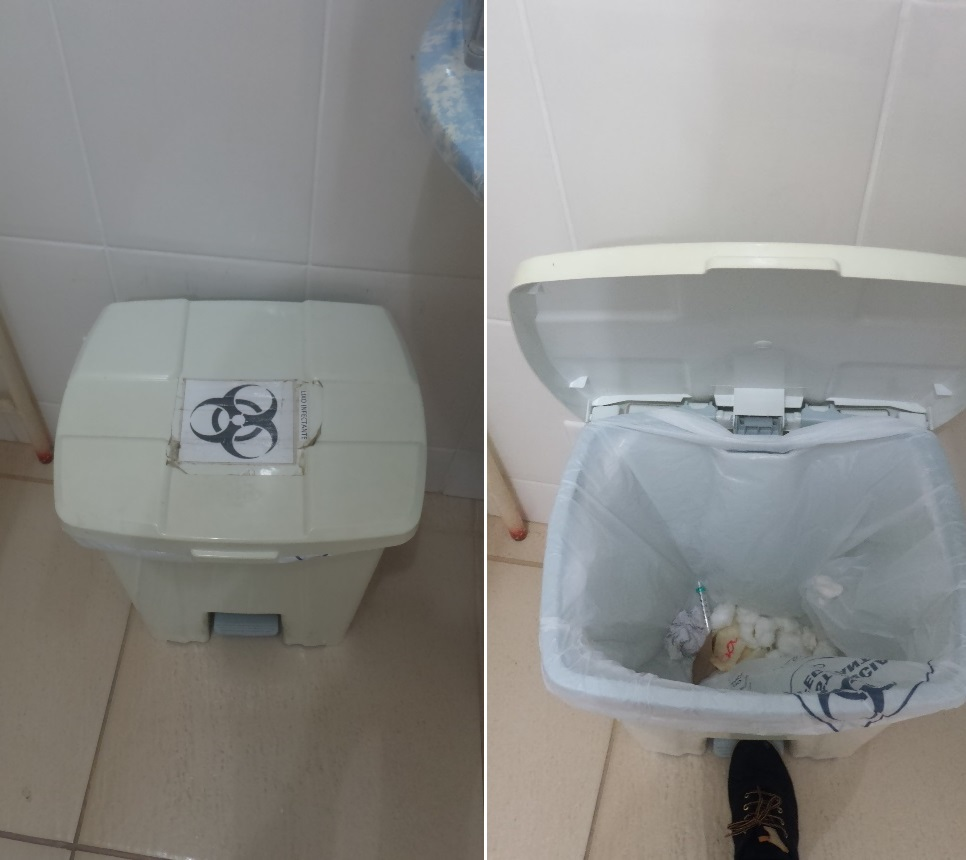
\includegraphics[width=0.75\linewidth]{produtos/prodtres/image066_67}
		\caption{Acondicionamento de resíduos de serviço de saúde contaminados da \gls{ubs}.}
		\legend{Fonte: Elaborado pelos autores.}
		\label{fig:image066_67}
	\end{figure}


	Os resíduos similares aos domiciliares, como dito anteriormente, são segregados entre comum e reciclável pela maioria dos estabelecimentos geradores de \gls{rss}. A \gls{ubs} segrega estes resíduos e alguns recipientes são envolvidos com sacos plásticos pretos, como mostrado na \autoref{fig:image068_69}. No entanto, alguns dos recipientes não apresentam não são envolvidos com nenhum saco plástico, como apresentado na \autoref{fig:image070_71}.

	\begin{figure}
		\centering
		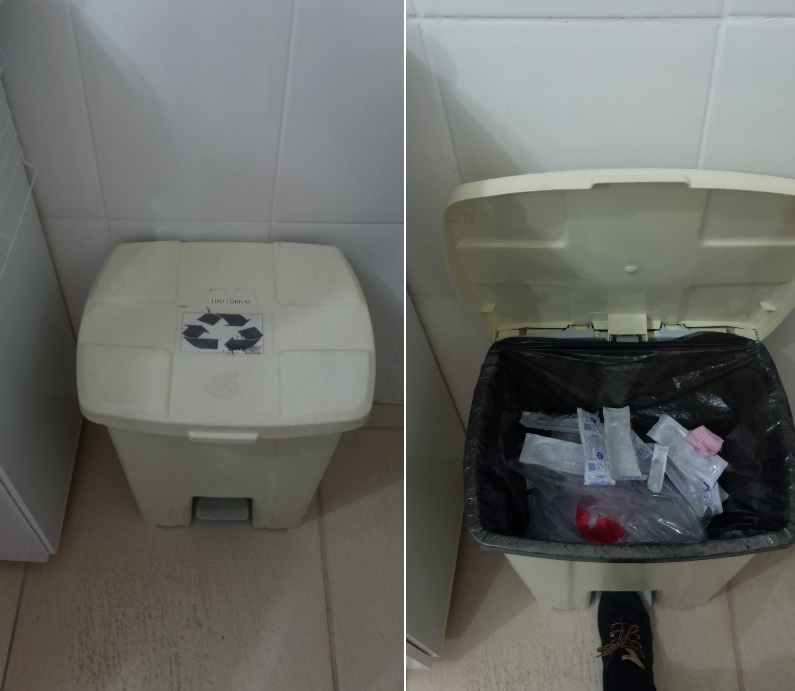
\includegraphics[width=0.75\linewidth]{produtos/prodtres/image068_69}
		\caption{Recipiente e acondicionamento de resíduos sólido similar ao domiciliar.}
		\legend{Fonte: Elaborado pelos autores.}
	\label{fig:image068_69}

	\end{figure}
	
	
	\begin{figure}
		\centering
		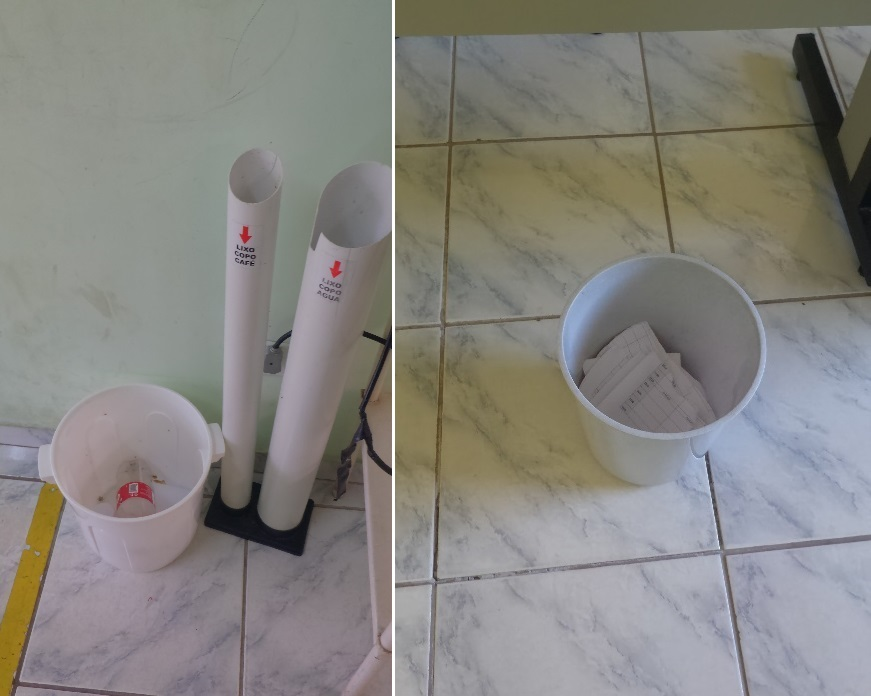
\includegraphics[width=0.75\linewidth]{produtos/prodtres/image070_71}
		\caption{Acondicionamento incorreto sem sacos plásticos de resíduos sólidos similares aos domiciliares.}
		\legend{Fonte: Elaborado pelos autores.}
		\label{fig:image070_71}
	\end{figure}


	Além disso, a cozinha da \gls{ubs} não dispõe de recipiente para descarte de resíduos orgânicos e recicláveis, o que faz com que seja descartado no recipiente disponível resíduos recicláveis (copos), orgânicos (cascas de frutas) e rejeitos (guardanapos usados) como revelado na \autoref{fig:image072}. 
	
	\begin{figure}
		\centering
		\includegraphics[width=0.40\linewidth]{produtos/prodtres/image072}
		\caption{Descarte de resíduos recicláveis, orgânicos e rejeitos no recipiente de resíduos sólidos da cozinha da \gls{ubs}.}
		\legend{Fonte: Elaborado pelos autores.}
		\label{fig:image072}
	\end{figure}
	
	
	A \gls{ubs} dispõe de local de armazenamento externo, apresentado na \autoref{fig:image073}, onde os resíduos gerados são armazenados até que os resíduos similares aos resíduos sólidos domiciliares (armazenados na primeira porta) sejam dispostos no muro para coleta ou até que os resíduos dos grupos A e E (armazenados na segunda porta) sejam coletados pela empresa terceirizada especializada.
	
	\begin{figure}
		\centering
		\includegraphics[width=0.40\linewidth]{produtos/prodtres/image073}
		\caption{Local de armazenamento temporário dos \gls{rss}.}
		\legend{Fonte: Elaborado pelos autores.}
		\label{fig:image073}
	\end{figure}
	
	
	De acordo com o recomendado pelo Manual de Gerenciamento de \gls{rss} da \gls{anvisa}, o local de armazenamento externo apresenta área suficiente para armazenamento dos resíduos, ambiente separado para armazenamento de resíduos do grupo D e do grupo A em conjunto com o Grupo E e condições para lavagem adequadas (pisos e paredes laváveis, ralos). No entanto, os sacos deveriam ser armazenados em recipientes rígidos ao invés de serem dispostos diretamente no piso, como apresentado na \autoref{fig:image074_75} \cite{anvisa_manualrss_2006}.
	
	\begin{figure}
		\centering
		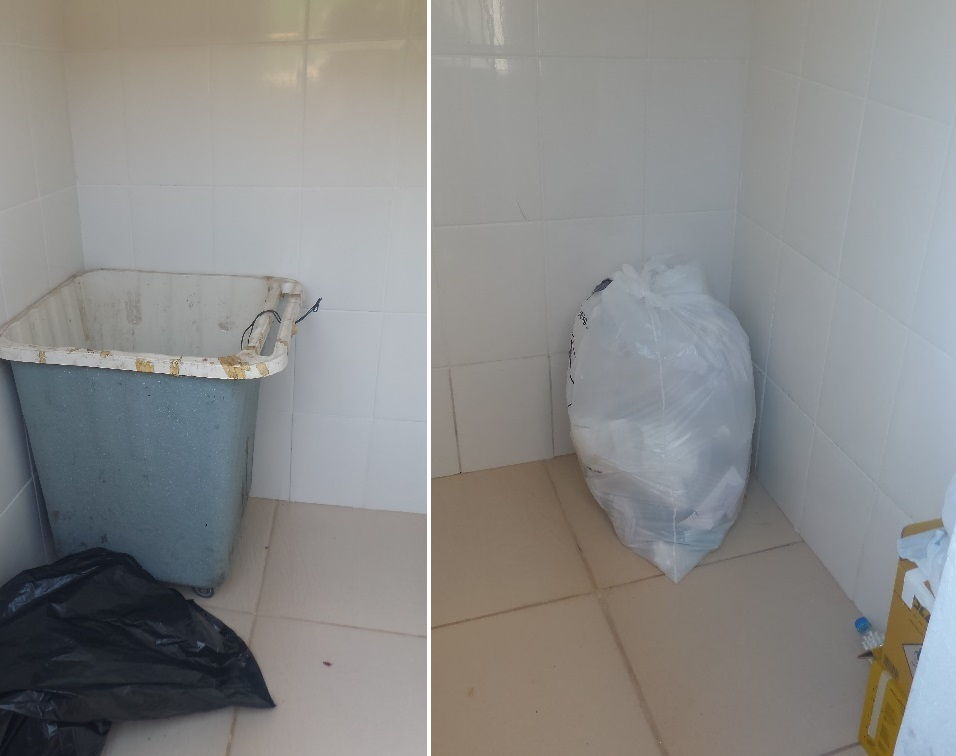
\includegraphics[width=0.75\linewidth]{produtos/prodtres/image074_75}
		\caption{Sacos armazenados diretamente no chão no local de armazenamento temporário.}
		\legend{Fonte: Elaborado pelos autores.}
		\label{fig:image074_75}
	\end{figure}

	
	Os resíduos compostos pelos grupos A e E são coletados pela empresa terceirizada AGIT Soluções Ambientais Ltda diretamente do local de armazenamento temporário.
	
	Os sacos plásticos contendo os resíduos sólidos comum e recicláveis são atualmente dispostos no muro da \gls{ubs} até que o serviço municipal de coleta seja realizado, como apresentado na \autoref{fig:image076}.
	
	\begin{figure}
		\centering
		\includegraphics[width=0.50\linewidth]{produtos/prodtres/image076}
		\caption{Local de armazenamento de resíduos sólidos comuns e recicláveis até o momento da coleta.}
		\legend{Fonte: Elaborado pelos autores.}
		\label{fig:image076}
	\end{figure}
	
	
	Para a segurança e higiene, seria recomendado que estes sacos fossem armazenados em cestas ou locais fechados até o momento da coleta. Os resíduos sólidos comuns e recicláveis são dispostos nos dias e horários das respectivas coletas, no entanto, devido ao horário restrito da coleta de resíduos recicláveis (terças e quintas no período da tarde), seria preferível que houvesse também cestas ou locais fechados específicos para cada um dos resíduos comum e reciclável.

	De acordo com o recomendado pelo Manual de gerenciamento da \gls{anvisa}, o local de armazenamento externo deveria apresentar \cite{anvisa_manualrss_2006}:
	
	\begin{description}
		\item [Acessibilidade] Ambiente que permita fácil acesso para recipientes de transporte e para os veículos coletores.
		\item[Exclusividade] Ambiente utilizado somente para armazenamento de resíduos.
		\item[Segurança] Ambiente deve ser seguro da ação de intemperes e do contato de animais e pessoas não autorizadas.
		Higiene e saneamento: Deve haver local para limpeza dos recipientes e contenedores, o ambiente deve apresentar iluminação, ventilação e pisos e paredes laváveis
	\end{description}

	\subsubsection{Coleta, transbordo e transporte} 
	Os estabelecimentos particulares geradores de \gls{rss} encaminham os resíduos classificados como grupo A e E para a \gls{ubs} de Monteiro Lobato, com exceção do veterinário 2, que encaminha estes resíduos para São José do Campos. Os resíduos do Grupo D gerados pelos estabelecimentos público e particulares são coletados pelo serviço de coleta público do município.
	
	A \gls{ubs} armazena no ambiente específico os resíduos de grupo A e E gerados e recolhidos e, de 15 em 15 dias a empresa AGIT Soluções Ambientais Ltda é responsável pela coleta, transporte para o município de Itajubá e disposição final destes resíduos.
	
	Através de entrevistas com os responsáveis pelos estabelecimentos veterinário, os donos são responsáveis pela disposição final do corpo do animal quando o mesmo vem à óbito quando tratado no veterinário 1, enquanto que o estabelecimento veterinário 2 ou costuma enterrar o cadáver do animal.
	
	\subsubsection{Disposição final}
	
	De acordo com o contrato realizado entre a Prefeitura e Monteiro Lobato e a empresa especializada AGIT Soluções Ambientais Ltda, a empresa é responsável pelo serviço de coleta, transporte e incineração dos resíduos de serviço de saúde de até 1.800 quilogramas coletados da \gls{ubs}.
	O contrato com a empresa especializada foi firmado em setembro de 2014 e têm sido anualmente prorrogado para os mesmos serviços por mais 12 meses até atualmente, no ano de 2017.
	
	\subsubsection{Volume}
	De acordo com os dados obtidos da série histórica do \gls{snis} para Monteiro Lobato, a \autoref{tab:massa_rss} foi elaborada com os dados de massa per capita coletada de \gls{rss} em relação a população urbana e a respectiva taxa de \gls{rss} coletada em relação aos \gls{rsu} coletados, englobando resíduo sólido comum, recicláveis e de limpeza urbana.
	
	\input{./produtos/prodtres/massa_rss}
	
	A empresa AGIT Soluções Ambientais Ltda disponibilizou os dados de peso em quilogramas mensais recolhidos de Monteiro Lobato do período de setembro de 2014, quando foi firmado o contrato, até o mês de dezembro de 2017. Considerando que os dados foram disponibilizados no meio do mês de dezembro, o valor cedido não representa toda a geração de \gls{rss} do mês.
	
	A \autoref{fig:image077} apresenta a geração per capita de \gls{rss} para os anos de 2014 a 2017 em função das médias anuais dos dados fornecidos pela AGIT Soluções Ambientais Ltda de peso recolhido de \gls{rss} de Monteiro Lobato.
	
	\begin{figure}
		\centering
		\includegraphics[width=0.75\linewidth]{produtos/prodtres/image077}
		\caption{Geração per capita de \gls{rss} do município de Monteiro Lobato.}
		\legend{Fonte: Elaborado pelos autores.}
		\label{fig:image077}
	\end{figure}
	
	
	Ao comparar os valores de geração per capita da \autoref{fig:image077} com os valores da \autoref{tab:massa_rss} observa-se uma diferença destoante. Esta diferença pode estar associada, em primeiro lugar, ao cálculo realizado pelo \gls{snis} para definição do indicador de geração per capita, pois é realizado em função da população urbana do município; enquanto que os valores, apresentados na \autoref{fig:image077}, foram determinados em função da população total estimada do município de acordo com o \gls{ibge}. Além disso, deve-se considerar que a quantidade recolhida pela empresa especializada na \gls{ubs} de Monteiro Lobato abrange os \gls{rss} de todos os estabelecimentos particulares geradores de \gls{rss} do município. 
	
	Em relação à quantidade total de \gls{rss} coletada, a \autoref{tab:quantidade_rss} foi elaborada a partir dos dados declarados ao \gls{snis} em toneladas \cite{snis_serie_2016}. Analisando os valores, observa-se um aumento significativo de quantidade coletada de \gls{rss} em Monteiro Lobato em 2014, o qual declarou coletar 5,5 toneladas ao ano.

	
	\input{./produtos/prodtres/quantidade_rss}
	
	A \autoref{fig:image078} apresenta os pesos em toneladas coletados de Monteiro Lobato pela AGIT Soluções Ambientais Ltda para o período de setembro de 2014 ao meio de dezembro de 2017. De acordo com os valores é possível verificar que a quantidade declarada por Monteiro Lobato ao \gls{snis} para o ano de 2014 talvez não seja a correta. Apesar de o valor total do ano de 2014 da \autoref{fig:image078} representar o peso recolhido apenas para os meses de setembro até dezembro, a tendência analisada para os pesos entre os anos de 2015 e 2017 possibilitam inferir que o peso coletado em 2014 deve ter sido próximo à 1,5 toneladas.
	
	\begin{figure}
		\centering
		\includegraphics[width=0.75\linewidth]{produtos/prodtres/image078}
		\caption{Quantidade de \gls{rss} em toneladas coletada anualmente em Monteiro Lobato.}
		\legend{Fonte: Elaborado pelos autores.}
		\label{fig:image078}
	\end{figure}
	
	
	Em 2007, o \gls{pmsb} de Monteiro Lobato mencionou que a geração média de \gls{rss} ao mês no município era de 150 kg \cite{ml_pmisb_2007}. A \autoref{fig:image079} que apresenta a quantidade recolhida em quilograma pela empresa especializada mensalmente para os anos de 2014 até 2017. Como o contrato com a empresa foi iniciado em setembro de 2014, não há valores referentes aos meses anteriores a setembro de 2014.
	
	\begin{figure}
		\centering
		\includegraphics[width=0.75\linewidth]{produtos/prodtres/image079}
		\caption{Relação de quantidade de \gls{rss} coletada mensalmente para os anos de 2014 a 2017 em Monteiro Lobato.}
		\legend{Fonte: Elaborado pelos autores.}
		\label{fig:image079}
	\end{figure}
	
	
	A \autoref{fig:image079} permite aferir que não há uma tendência clara em relação à geração de \gls{rss} ao longo dos anos e ao longo dos meses, com exceção do mês de junho, que apresentou a menor geração para os três anos com dados. A \autoref{fig:image018}, que apresenta a mesma relação para o \gls{rsu}, revela também uma queda na geração de resíduos no inverno, porém a redução foi mais discreta que a verificada para o \gls{rss} na \autoref{fig:image079}.

	Seguindo a mesma tendência, a maior geração de \gls{rss} entre os meses de outubro e março pode ser justificada pela presença de população flutuante de turistas na região. Porém, como quase todos os estabelecimentos particulares geradores de \gls{rss} costumam encaminhar seus resíduos de grupos A e E à \gls{ubs}, todos estes dados de geração abrangem estes resíduos. Como a \gls{ubs} não dispõe de um controle do peso de \gls{rss} recolhido dos estabelecimentos particulares, é difícil inferir a tendência que os pesos disponibilizados pela AGIT significam.

	Uma hipótese para os maiores valores de \gls{rss} gerados em 2017 pode ser referente à abertura de um novo estabelecimento particular gerador de \gls{rss} que passou a encaminhar os resíduos à \gls{ubs}. Neste contexto, é importante que o município possua de um sistema de cadastro de todos os estabelecimentos geradores de \gls{rss}, além de dispor de um controle da quantidade de resíduos que cada um destes estabelecimentos encaminha à \gls{ubs}. 

	A elaboração deste \gls{pmgirs} é imprescindível para que a dinâmica de geração de resíduos sólidos seja conhecida e para colaborar com um sistema diferenciado de coleta mais adequado.

	
	\subsection{Resíduos Agrossilvipastoris}
	\label{sub_agro}
	
	Os resíduos agrossilvipastoris podem ser definidos como os resíduos gerados nas atividades agropecuárias e silviculturais, assim como os insumos utilizados nestas atividades \cite{brasil:12305}. Estes resíduos podem ser divididos em resíduos orgânicos e inorgânicos.
	
	\subsubsection{Resíduos Agrossilvipastoris orgânicos}
	São fontes de resíduos orgânicos, de acordo com o \gls{pnrs} \cite{mma_pnrs_2012}:
	
	\begin{itemize}
		\item Agroindústria associada à agricultura: culturas de soja, milho, cana de açúcar, feijão, arroz, trigo, mandioca, café, cacau, banana, laranja, uva, outros;
		\item Pecuária: criação de aves (postura e corte), suínos e bovinos (leite);
		\item Agroindústria associada à pecuária: abatedouros de aves, suínos e bovinos, graxaria e laticínios.
		\item Agroindústria associada ao setor florestal.
	\end{itemize}
	
	Os resíduos florestais abrangem material proveniente da colheita ou de processamento da madeira e de outros produtos florestais que permanecem sem utilização durante o processo tanto por conta de limitações tecnológicas ou de mercados, sendo descartados durante a produção \cite{nolasco_colheita_2000}. 
	
	Os resíduos de madeira são classificados como resíduos lignocelulósicos por apresentar em sua composição, majoritariamente, lignina e celulose, os quais são oriundos de atividades industriais quanto de atividades rurais \cite{teixeira_materiais_2005}.
	
	As carcaças de animais mortos são resíduos caracterizados pelo Grupo A que, de acordo com a Resolução CONAMA n°358/2005, engloba os resíduos com possível presença de agentes biológicos e risco de infecção. Devido à composição destes resíduos e considerando que estes não podem ser reciclados, reutilizados ou reaproveitados, a disposição final ambientalmente adequada é de suma importância para a saúde pública \cite{conama:358}.
	
	Sendo usualmente do grupo A4, as carcaças de animais advindas do setor agropecuário podem ser dispostas em local devidamente licenciado sem tratamento prévio. A necessidade do tratamento fica a critério do órgão ambiental responsável \cite{conama:358}.
	
	\subsubsection{Resíduos Agrossilvipastoris inorgânicos}
	
	As fontes de resíduos inorgânicos, por outro lado, \cite{mma_pnrs_2012}, são classificados:
	
	\begin{itemize}
		\item 	Embalagens de agrotóxicos;
		\item   Embalagens de fertilizantes;
		\item 	Insumos farmacêuticos veterinários;
		\item   Resíduos sólidos domésticos da área rural.
	\end{itemize}

	Um dos resíduos inorgânicos gerados através das atividades agropecuárias são as embalagens de defensivos agrícolas. Devido aos riscos ambientais que as embalagens de agrotóxicos e fertilizantes oferecem, as mesmas são itens de logística reversa obrigatória, e tem seu manejo orientado pelo Decreto Nº 4.074, de 4 de janeiro de 2002 \cite{brasil:4074}. Contudo, nota-se uma carência de legislações sobre o produto.
	
	Os insumos farmacêuticos para atividades pecuárias consistem de medicamentos de uso veterinários e suplementos alimentares animais, englobando assim o remédio propriamente, as embalagens, ampolas e agulhas. De acordo com o \gls{sindan} são divididos em biológicos, antimicrobianos, terapêuticos, tônicos/fortificantes, desinfetantes, dermatológicos e outros \cite{sindan_2011}.
	
	De acordo com o Art. 20 da \gls{pnrs}, os responsáveis por atividades agrossilvipastoris devem elaborar um plano de gerenciamento de resíduos sólidos em caso de exigência de órgão competente do \gls{sisnama}, \gls{snvs} ou \gls{suasa} \cite{brasil:12305}.
	
	Os usuários dos agrotóxicos possuem responsabilidade por algumas etapas do processo de logística reversa do material como a lavagem tríplice da embalagem, correto armazenamento temporário, transporte até o local de aquisição e o armazenamento da nota fiscal ou comprovante de entrega das embalagens por até um ano \cite{brasil:9974}. Para isso, os canais de distribuição têm a competência de orientar o consumidor de como realizar os procedimentos, além de disponibilizar na nota o endereço correto para entrega das embalagens vazias \cite{conama:334}.
	
	De acordo com a Lei nº 9.974/2000, compete à indústria fabricante o recolhimento das embalagens nos canais de distribuição, destinar de maneira adequada as embalagens e alterar os rótulos e bulas de seus produtos para que contenham informações sobre o que compete ao usuário e como ele deve realizar sua parte. Aos órgãos públicos compete a criação de programas de incentivo e educação ambiental para maximizar a quantidade de embalagens devolvidas bem como realizar a devida fiscalização sobre os processos envolvidos na logística reversa \cite{brasil:9974}.
	
	A disposição final ambientalmente adequada de carcaças de animais mortos deve ser realizada de acordo com as diretrizes apresentadas pela Resolução CONAMA n°358/2005 e a fiscalização de seu manejo é de responsabilidade dos órgãos ambientais competentes integrantes do \gls{sisnama} \cite{brasil:12305}.
	
	De acordo com o \gls{lspa} realizado pelo \gls{ibge}, o Brasil possui uma área plantada de 121.552.319 hectares, gerando uma quantidade de 1.168.413.127 toneladas de produtos \cite{ibge_lspa_2017}. A significativa quantidade de área destinada à agropecuária no país indica a sua importância econômica, fato esse que leva ao uso de agrotóxicos e fertilizantes com fim de garantir uma safra mais produtiva. Entretanto, os insumos utilizados são considerados potenciais poluidores do meio ambiente e são objetos de logística reversa obrigatória. Neste contexto, em 2001 foi fundado o \gls{inpev}, responsável pela coleta das embalagens pós utilização.	
	No ano de 2016, 44.528 toneladas de embalagens vazias de defensivos agrícolas foram recolhidas e foram destinadas de modo ambientalmente adequado, representando 94 \% do total das embalagens primárias comercializadas. Destes 94 \%, 90 \% das embalagens são enviadas para reciclagem, enquanto que 4 \% são encaminhados para incineração \cite{abrelpe_panorama_2016}. A \autoref{fig:image080} mostra a evolução do recolhimento de embalagens de defensivos em toneladas \cite{inpev_quemsomos_2019}.
	
	\begin{figure}
		\centering
		\includegraphics[width=0.75\linewidth]{produtos/prodtres/image080}
		\caption{Embalagens de Defensivos Agrícolas Recolhidas pelo InpEV.}
		\legend{Fonte: Adaptado de Abrelpe, 2016}
		\label{fig:image080}
	\end{figure}
	
	
	Através de uma estimativa realizada levando em consideração a quantidade de fertilizantes utilizadas e as áreas das \gls{upa}, o \gls{ipea} infere que a quantidade de embalagens de fertilizantes utilizadas no país, em 2010 foi, de cerca de 64,2 milhões, evidenciando a importância de políticas que regulamentem a sua destinação final correta, diminuindo assim os seus riscos de contaminação ao homem e ao meio ambiente \cite{ipea_diagagro_2013}.

	Em contato com o Sindicato Rural de Monteiro Lobato, foi averiguado que os produtores rurais adquirem defensivos agrícolas através loja Verdevale Comércio Agropecuário, localizada em São José dos Campos. No entanto, não existe controle por parte da prefeitura ou do fornecedor da quantidade consumida de defensivos agrícolas pelo município. 
	
	A responsabilidade do retorno das embalagens dos defensivos é do produtor e a devolução deve ser realizada na Central de Recebimento de Embalagens Vazias de Defensivos Agrícola do município de Taubaté até o prazo de um ano da compra para constituir a logística reversa.
	
	O \gls{lupa} aponta que, em 2008 foram contabilizadas 304 unidades de produção no município de Monteiro Lobato, totalizando uma área de 26.162,8 hectares \cite{sp_lupa:2008}. Dentre as \gls{upa} contabilizadas, as utilizações são mostradas na \autoref{tab:upas}.
	
	\input{./produtos/prodtres/upas}

	Os cultivos realizados nas \gls{upa} e as respectivas áreas mínimas, médias e máximas são mostrados na \autoref{tab:cultivos_upas}.
	
	% Table generated by Excel2LaTeX from sheet 'cultivos_upa'
\begin{table}[htbp]
  \centering
  \caption{Cultivos Realizados nas UPAs de Monteiro Lobato.}
    \begin{tabular}{p{14.5em}|c|c|c|c|c}
    \rowcolor[rgb]{ .969,  .588,  .275} \textcolor[rgb]{ 1,  1,  1}{\textbf{CULTURA}} & \multicolumn{1}{P{4.215em}|}{\textcolor[rgb]{ 1,  1,  1}{\textbf{N. de UPA}}} & \multicolumn{1}{P{4.215em}|}{\textcolor[rgb]{ 1,  1,  1}{\textbf{Área mínima (ha)}}} & \multicolumn{1}{P{4.215em}|}{\textcolor[rgb]{ 1,  1,  1}{\textbf{Área média (ha)}}} & \multicolumn{1}{P{5.07em}|}{\textcolor[rgb]{ 1,  1,  1}{\textbf{Área máxima (ha)}}} & \multicolumn{1}{P{5.43em}}{\textcolor[rgb]{ 1,  1,  1}{\textbf{TOTAL}}} \\
    \rowcolor[rgb]{ .984,  .831,  .706} \textbf{Braquiária} & 254   & 1     & 43,7  & 1.500,00 & 11.110,20 \\
    \rowcolor[rgb]{ .992,  .914,  .851} \textbf{Eucalipto} & 59    & 0,3   & 57,2  & 1.000,00 & 3.376,50 \\
    \rowcolor[rgb]{ .984,  .831,  .706} \textbf{Outras gramíneas para pastagem} & 30    & 0,3   & 79,5  & 1.500,00 & 2.386,40 \\
    \rowcolor[rgb]{ .992,  .914,  .851} \textbf{Capim-gordura} & 18    & 3     & 25,7  & 72,8  & 462,9 \\
    \rowcolor[rgb]{ .984,  .831,  .706} \textbf{Gramas} & 8     & 2,3   & 39,3  & 191   & 314,3 \\
    \rowcolor[rgb]{ .992,  .914,  .851} \textbf{Capim-napier (capim-elefante)} & 30    & 0,4   & 1,7   & 5     & 50,8 \\
    \rowcolor[rgb]{ .984,  .831,  .706} \textbf{Banana} & 21    & 0,4   & 1,8   & 7,2   & 38,1 \\
    \rowcolor[rgb]{ .992,  .914,  .851} \textbf{Cana-de-açúcar} & 17    & 0,3   & 1,9   & 5     & 32,3 \\
    \rowcolor[rgb]{ .984,  .831,  .706} \textbf{Outras culturas temporárias} & 1     & 23,4  & 23,4  & 23,4  & 23,4 \\
    \rowcolor[rgb]{ .992,  .914,  .851} \textbf{Milho} & 13    & 0,2   & 1,3   & 3     & 17,4 \\
    \rowcolor[rgb]{ .984,  .831,  .706} \textbf{Outras frutíferas} & 10    & 0,5   & 1,5   & 4     & 14,9 \\
    \rowcolor[rgb]{ .992,  .914,  .851} \textbf{Café} & 7     & 0,5   & 2,1   & 6     & 14,5 \\
    \rowcolor[rgb]{ .984,  .831,  .706} \textbf{Pomar doméstico} & 11    & 0,5   & 0,6   & 1     & 7,1 \\
    \rowcolor[rgb]{ .992,  .914,  .851} \textbf{Mandioca} & 5     & 0,5   & 1,1   & 2     & 5,5 \\
    \rowcolor[rgb]{ .984,  .831,  .706} \textbf{Laranja} & 3     & 1     & 1,1   & 1,2   & 3,2 \\
    \rowcolor[rgb]{ .992,  .914,  .851} \textbf{Feijão} & 2     & 1     & 1,3   & 1,5   & 2,5 \\
    \rowcolor[rgb]{ .984,  .831,  .706} \textbf{Milho-silagem} & 1     & 2     & 2     & 2     & 2 \\
    \rowcolor[rgb]{ .992,  .914,  .851} \textbf{Limão} & 1     & 1,2   & 1,2   & 1,2   & 1,2 \\
    \rowcolor[rgb]{ .984,  .831,  .706} \textbf{Colonião} & 1     & 1     & 1     & 1     & 1 \\
    \rowcolor[rgb]{ .992,  .914,  .851} \textbf{Outras flores} & 1     & 1     & 1     & 1     & 1 \\
    \rowcolor[rgb]{ .984,  .831,  .706} \textbf{Jabuticaba} & 1     & 0,3   & 0,3   & 0,3   & 0,3 \\
    \end{tabular}%
  \label{tab:cultivos_upas}%
  \legend{Fonte: Adaptado de ESTADO DE SÃO PAULO, 2007/2008.}
\end{table}%

	
	Analisando a \autoref{tab:cultivos_upas}, pode-se notar que as culturas mais significativas para o município são braquiárias, eucaliptos, gramíneas para pastagem e o capim-naiper e quanto a pecuária, destacam-se as criações de gado (leite e corte), equinos e suínos. As culturas de eucaliptos e capim podem apresentar como resíduo gerado materiais orgânicos como restos de madeiras e folhas.
	
	A \autoref{tab:exploracao_animal} por sua vez, mostra a exploração de animais no município.
	
	\input{./produtos/prodtres/exploracao_animal}
	
	Assim, pode-se observar que em relação a pecuária, a parcela mais significativa no município são as criações de gado (leite e corte), equinos e suínos. A criação destes animais pode implicar na geração de resíduos orgânicos como fezes e carcaças de animais mortos.
	
	De acordo com a resposta do ofício encaminhado à prefeitura com questionário estruturado sobre o manejo de carcaças de animais mortos, foi informado que na identificação de animais mortos de grande porte, que ocorre cerca de duas vezes ao mês, a \gls{smaa} e a \gls{ssm} são acionadas. Normalmente o procedimento seguido é a remoção do animal através de uma retroescavadeira acompanhado pelo motorista e por um profissional veterinário. Após a retirada, a carcaça é enterrada no solo.
	
	\subsubsection{Volume}
	O município de Monteiro Lobato não dispõe de um controle específico de geração dos demais resíduos orgânicos, de insumos farmacêuticos, de embalagens agrícolas e similares aos domiciliares gerados pelo setor agrossilvipastoril.
	
	\subsection{Resíduos da Construção Civil e Volumosos Inservíveis}
	\gls{rcc} são aqueles gerados das atividades de construções, reformas, reparos e demolições de obras de construção civil, incluindo os resíduos derivados da preparação e escavação de terrenos para obras civis, tais como: tijolos, blocos cerâmicos, concreto em geral, solos, rochas, metais, resinas, colas, tintas, madeiras e compensados, forros, argamassa, gesso, telhas, pavimento asfáltico, vidros, plásticos, tubulações, fiação elétrica, entre outros. Os \gls{rcc} são comumente denominados de entulhos de obras, caliça ou metralha \cite{brasil:12305, conama:307}. Os \gls{rcc} são divididos nas seguintes classes apresentadas na \autoref{tab:classificacao_rcc}.
	
	\input{./produtos/prodtres/classificacao_rcc}
	
	Os municípios são responsáveis pela implementação do plano de gerenciamento integrado de \gls{rcc} bem como pelas diretrizes, procedimentos e critérios para o manejo adequado do \gls{rcc} \cite{conama:307}. 
	
	O plano de gerenciamento integrado de \gls{rcc} deverá incorporar \cite{conama:307}:
	
	\begin{itemize}
		\item Programa Municipal de Gerenciamento de \gls{rcc} com as diretrizes técnicas e procedimentos para o exercício das responsabilidades dos pequenos geradores e transportadores;
		\item Projetos de Gerenciamento de \gls{rcc} que orientem, disciplinem e expressem o compromisso de ação correta por parte dos grandes geradores de resíduos, tanto públicos quanto privados.
	\end{itemize}

	Neste contexto, cabe aos municípios a solução para os pequenos volumes, geralmente maldispostos, e o disciplinamento da ação dos agentes envolvidos com o manejo dos grandes volumes de resíduos.

	Para os estabelecimentos classificados pelo município como grandes geradores e para geradores de \gls{rcc} caracterizados como perigosos compete ao município a orientação a de como elaborar um plano de gerenciamento de \gls{rcc} \cite{brasil:12305}. Entretanto, Monteiro Lobato não dispõe de legislação que caracterize pequenos e grandes geradores.

	Dos 5.570 municípios brasileiros, 4.031 apresentam serviço de manejo dos \gls{rcc} e apenas 392 possuem de alguma forma de processamento desse resíduo, como apresenta a \autoref{tab:manejo_rcc} \cite{ipea_diagrcc_2012}. 
	
	% Table generated by Excel2LaTeX from sheet 'manejo_rcc'
\begin{table}[htbp]
  \centering
  \caption{Informação sobre o tipo de processamento entre os 392 municípios brasileiros com serviço de manejo de RCC.}
    \begin{tabular}{P{28.07em}|c}
    \rowcolor[rgb]{ .969,  .588,  .275} \textcolor[rgb]{ 1,  1,  1}{\textbf{Tipos de Processamento}} & \multicolumn{1}{P{6.645em}}{\textcolor[rgb]{ 1,  1,  1}{\textbf{Quantidade}}} \\
    \rowcolor[rgb]{ .992,  .914,  .851} Reaproveitamento dos agregados produzidos na fabricação de componentes construtivos & 79 \\
    \rowcolor[rgb]{ .984,  .831,  .706} Triagem e trituração simples dos resíduos Classe A, com classificação granulométrica dos agregados reciclados & 20 \\
    \rowcolor[rgb]{ .992,  .914,  .851} Triagem e trituração simples dos resíduos Classe A & 14 \\
    \rowcolor[rgb]{ .984,  .831,  .706} Triagem simples dos resíduos de construção e demolição reaproveitáveis (classes A e B) & 124 \\
    \rowcolor[rgb]{ .992,  .914,  .851} Outros & 204 \\
    \end{tabular}%
  \label{tab:manejo_rcc}%
  \legend{Fonte: Adaptado de (INSTITUTO DE PESQUISA ECONÔMICA APLICADA, 2012).}
\end{table}%

	
	Segundo pesquisa realizada pelo \gls{snis}, em uma amostra de 372 municípios do Brasil, a quantidade de \gls{rcc} coletada no ano de 2008 foi de 14.557.939, 22 tonelada/ano. A caracterização estimada dos materiais constituintes de \gls{rcc} no Brasil foi: argamassa (63 \%), concreto e blocos (29 \%), outros (7 \%) e orgânicos (1 \%) \cite{ipea_diagrcc_2012}. O Brasil, no ano de 2014, possuía unidades para área de transbordo e triagem de \gls{rcc} e volumosos, reciclagem e aterro de \gls{rcc} de acordo com a \autoref{tab:unidade_rcc} \cite{snis_diag_2014}. 
	
	\input{./produtos/prodtres/unidade_rcc}
	
	De acordo com levantamento do Diagnóstico de \gls{rcc} realizado pelo \gls{ipea} e publicado no ano de 2012, é estimado que o Brasil gere uma média de 31 milhões de toneladas ao ano de \gls{rcc} \cite{ipea_diagrcc_2012}. A \gls{abrelpe}, que apresenta dados mais atualizados, revela que no ano de 2016 foram coletados no Brasil 45,1 milhões de tonelada de \gls{rcc}, sendo que a Região Sudeste foi responsável pela coleta de 23,35 milhões de toneladas de \gls{rcc}, representando quase metade do total coletado no país \cite{abrelpe_panorama_2016}.	
	
	Atualmente, a \gls{ssm} de Monteiro Lobato é responsável pela coleta dos \gls{rcc}. O serviço prestado pela prefeitura é taxado do solicitante através da cobrança de R\$ 41,82 por hora de serviço e por R\$ 25,09 por hora do uso do caminhão basculante. Os dados de quantidade de \gls{rcc} coletada e suas respectivas taxas não foram declarados na base \gls{snis} nos anos de 2009 a 2015, mostrando que ainda há uma deficiência no controle e catalogação de dados, dificultando assim, sua posterior análise e possíveis ações de melhoria para o manejo desse tipo de resíduo.
	
	\subsubsection{Acondicionamento}
	Os \gls{rcc} gerados são armazenados na calçada em frente ao imóvel da respectiva construção civil até que seja realizada a coleta pela \gls{ssm}, como ilustra a \autoref{fig:image081} (parte superior: área localizada próxima à rodoviária; parte inferior: área em frente a \gls{ssm}). Após a coleta, os \gls{rcc} são armazenados ao ar livre no pátio da prefeitura no bairro Morada do Sol até que seja realizada a destinação final.
	
	\begin{figure}
		\centering
		\includegraphics[width=0.75\linewidth]{produtos/prodtres/image081}
		\caption{\gls{rcc} disposto na calçada para coleta.}
		\legend{Fonte: Elaborado pelos autores.}
		\label{fig:image081}
	\end{figure}
	
	
	\subsubsection{Coleta, transbordo e transporte dos Resíduos da Construção Civil}
	A coleta do \gls{rcc} é realizada às sextas-feiras por quatro funcionários, através de retroescavadeiras, enxada, enxadão e pá. O \gls{rcc} é colocado em um caminhão basculante com capacidade de 5 m³, o qual transporta este resíduo ao pátio da prefeitura, localizado no bairro Morada do Sol (vide \autoref{fig:image082}).
	
	\begin{figure}
		\centering
		\includegraphics[width=0.7\linewidth]{produtos/prodtres/image082}
		\caption{Transbordo de \gls{rcc} de Monteiro Lobato.}
		\legend{ Fonte: Elaborado pelos autores.}
		\label{fig:image082}
	\end{figure}
	
	
	A \autoref{fig:image083} apresenta a disposição dos \gls{rcc} no pátio, observa-se a disposição inadequada dos resíduos em solo exposto e ao ar livre. Além de \gls{rcc}, é possível verificar a disposição incorreta de pneus em solo exposto e em área aberta.

	\begin{figure}
		\centering
		\includegraphics[width=0.7\linewidth]{produtos/prodtres/image083}
		\caption{Disposição de \gls{rcc} no pátio morada do sol.}
		\legend{Fonte: Elaborado pelos autores.}
		\label{fig:image083}
	\end{figure}
	
	
	\subsubsection{Disposição final}
	De acordo com a \gls{ssm}, os \gls{rcc} que ficam armazenados no pátio da prefeitura, quando necessário, são utilizados em estradas vicinais e nas valetas e buracos com erosões. Os resíduos volumosos (como sofás, armários e camas) são destinados ao aterro sanitário de Tremembé, em conjunto com os resíduos sólidos comum.
	
	Foi possível verificar em pesquisa de campo que o município, apesar apresentar o serviço de coleta, ainda apresenta uma disposição final inadequada destes resíduos. A \autoref{fig:image084} apresenta uma área de solo exposto próximo à uma área florestal com \gls{rcc} disposto ao ar livre, apesar da placa de indicação que é proibido descartar este tipo de resíduo.
	
	\begin{figure}
		\centering
		\includegraphics[width=0.7\linewidth]{produtos/prodtres/image084}
		\caption{Disposição final inadequada de \gls{rcc} em solo exposto.}
		\legend{Fonte: Elaborado pelos autores.}
		\label{fig:image084}
	\end{figure}
	
	
	Além da disposição de \gls{rcc} em solos expostos, foi observada uma tendência na disposição inadequada de \gls{rcc} principalmente ao redor de lixeiras principalmente próximas à estrada, como apresentada na \autoref{fig:image085}.

\clearpage	
	\begin{figure}
		\centering
		\includegraphics[width=0.4\linewidth]{produtos/prodtres/image085}
		\caption{\gls{rcc} e resíduos de maior porte dispostos em solo.}
		\legend{Fonte: Elaborado pelos autores.}
		\label{fig:image085}
	\end{figure}

	
	\subsubsection{Volume}
	O município de Monteiro Lobato não dispõe de controle sobre o volume ou peso de \gls{rcc} coletados periodicamente. De acordo com a \gls{ssm}, este valor é muito variável.
	
	
	\subsection{Resíduos de Serviços de Transportes}
	
	São considerados resíduos de serviço de transporte aqueles provenientes de portos, aeroportos, terminais alfandegários, rodoviários, ferroviários e passagens de fronteira. Os resíduos gerados nesses locais são de natureza séptica, podendo conter organismos patogênicos, como materiais de higiene pessoal e restos de comida, além de resíduos de outra natureza. Os resíduos sépticos dos resíduos de serviço de transporte podem transmitir doenças de outras cidades, estados e países devido à grande circulação de pessoas de diferentes locais nestes terminais \cite{brasil:12305}.
	
	Os responsáveis pelos estabelecimentos geradores de resíduos de serviço de transporte deverão elaborar um \gls{pgrs} nos termos do regulamento ou de normas estabelecidas pelos órgãos do Sisnama e, se couber, do \gls{snvs} \cite{brasil:12305}.
	
	Uma pesquisa realizada no Brasil em novembro de 2010 pelo Programa Despoluir \cite{cnt_despoluir_2010}, abordou 649 empresas de transporte rodoviário de passageiros e cargas e constatou que um dos problemas mais recorrentes enfrentado pelas transportadoras é a gestão de resíduos. A dificuldade principal está no alto custo do descarte ambientalmente adequado além da falta de empresas especializadas e licenciadas para realizar essa atividade. Este problema se agrava ainda mais nos locais mais afastados dos grandes centros e nas regiões Norte e Nordeste \cite{cnt_despoluir_2010}.
	
	Aproximadamente 89 \% das empresas de transporte já possuem ações ambientais atreladas ao seu planejamento operacional ou possuem \gls{sga}. Geralmente, as empresas transportadoras de grande porte (frota maior que 100 veículos) possuem iniciativas e ações de cunho sustentável e apresentam um percentual de 45 \% com um \gls{sga}. Das pequenas empresas (até 5 veículos), apenas 6 \% possui boas práticas e 1 \% possui \gls{sga} \cite{paixao_rstransporte_2011}.
	
	O município de Monteiro Lobato dispõe de um único terminal rodoviário, apresentado na \autoref{fig:image086}, o qual é administrado pela \gls{pmml} através da \gls{ssm}. O Terminal Rodoviário, de acordo com resposta a \gls{ssm}, apresenta área construída de 432 m² e uma circulação mensal de aproximadamente cinco mil pessoas. As linhas municipais atendidas são apenas Centro x Bairro dos Souzas e Centro x Bairro de São Benedito, enquanto que as linhas intermunicipais atendidas são com destino à São José dos Campos e à São Francisco Xavier.
	
	\begin{figure}
		\centering
		\includegraphics[width=0.7\linewidth]{produtos/prodtres/image086}
		\caption{Terminal Rodoviário do Município de Monteiro Lobato.}
		\legend{Fonte: Elaborado pelos autores.}
		\label{fig:image086}
	\end{figure}
	
	
	\subsubsection{Acondicionamento}
	O terminal dispõe de um único cesto de resíduo compartilhado na área interna e dois cestos, iguais aos cestos distribuídos pelo município, localizados próximos ao ponto de táxi na área externa (vide \autoref{fig:image087}), os quais possuem sacos plásticos de 100 litros. O Terminal Rodoviário dispõe de dois sanitários (masculino e feminino) com três cabines cada. Cada sanitário apresenta 2 cestos de lixo grandes e três cestos de lixo apresentadas na \autoref{fig:image088}, um para cada cabine.
	
	\begin{figure}
		\centering
		\includegraphics[width=0.4\linewidth]{produtos/prodtres/image087}
		\caption{Formas de acondicionamento dos resíduos gerados no terminal central na área interna (a) e na área externa (b).}
		\legend{Fonte: Elaborado pelos autores.}
		\label{fig:image087}
	\end{figure}
	
	
	\begin{figure}
		\centering
		\includegraphics[width=0.5\linewidth]{produtos/prodtres/image088}
		\caption{Cesto de lixo dos sanitários feminino e masculino.}
		\legend{Fonte: Elaborado pelos autores.}
		\label{fig:image088}
	\end{figure}
	
	
	\subsubsection{Coleta, transbordo e transporte}
	A limpeza e conservação do Terminal são realizadas por três funcionários. Estes mesmos funcionários são responsáveis pela retirada dos sacos de lixo e pela triagem dos resíduos entre recicláveis e não recicláveis. A triagem é realizada no próprio terminal e os funcionários usam de bota de borracha, avental e luvas. Após a separação dos resíduos, os resíduos sólidos recicláveis e comuns são acondicionados em sacos plásticos de 100 litros e armazenados no pátio da garagem da \gls{ssm} até que seja realizado o serviço de coleta.
	
	\subsubsection{Disposição final}
	A coleta dos resíduos gerados pelo terminal é realizada pelo serviço de coleta do Município e segue a mesma destinação que os resíduos sólidos domiciliares, comum e reciclável. 
	
	\subsubsection{Volume}
	O terminal rodoviário não dispõe de um plano de gerenciamento de resíduos sólidos e não há o acompanhamento da quantidade gerada de resíduos sólidos e da respectiva caracterização. No entanto, sabe-se que normalmente são retirados, semanalmente, sete sacos plásticos de 100 litros de resíduo sólido comum e dois sacos plásticos de 100 litros de resíduo sólido reciclável. Neste contexto, é possível afirmar que, diariamente, são retirados aproximadamente 128 litros de resíduos sólido.

	O município de Monteiro Lobato não dispõe de regulamento que determine pequenos ou grandes geradores de resíduo sólidos através da geração de volume. Apesar disso, considerando que normalmente são considerados pequenos geradores estabelecimentos que geram até 120 litros de resíduo sólido por dia e, grandes geradores os estabelecimentos que geram um volume acima deste limite, o Terminal Rodoviário se aproxima das condições de pequeno gerador, mas seria caracterizado como grande gerador de acordo com estas condições \cite{ibam_manualrs_2001}.
	
	
	\subsection{Resíduos de Mineração}
	Os resíduos de mineração podem ser definidos como provenientes de atividades de pesquisa, extração (estéril) ou beneficiamento de minérios (rejeitos), sendo exemplos destes resíduos as pilhas de minérios pobres, estéreis, rochas, sedimentos, solos, aparas, lamas das serrarias de mármore ou granito, polpas de decantação de efluentes, sobras da mineração artesanal de pedras preciosas e semipreciosas e finos e ultrafinos não aproveitados no beneficiamento \cite{ibram_rejeitosmin_2016}. Entretanto, a maior parte da disposição dos rejeitos da mineração mundial se dá por barragens, cujo objetivo principal é a contenção do mesmo \cite{dnpm:70389, ibram_rejeitosmin_2016}.
	
	Devem ser considerados também os resíduos oriundos da operação das plantas de mineração, englobando os efluentes das estações de tratamento, pneus, lâmpadas, baterias, sucatas e resíduos de óleo em geral \cite{ibram_rejeitosmin_2016}. Os principais fatores que interferem na quantidade de resíduos sólidos da atividade de mineração são o processo de extração, a concentração da substância mineral na rocha matriz e a profundidade da jazida \cite{ipea_diagmineracao_2012}.
	
	É de competência do gerador a elaboração do plano de gerenciamento de resíduos sólidos, o conteúdo mínimo para tal documento está descrito no Art. 21 da \gls{pnrs} \cite{brasil:12305}.
	
	Em casos de disposição de rejeitos em reservatórios criados por barragens, a \gls{pnsb} designa o empreendedor como responsável legal pela segurança da barragem, cabendo a ele a prática de ações para garanti-la, como a obrigatoriedade da elaboração, implementação e constante atualização periódica do Plano de Segurança da Barragem, ferramenta da \gls{pnsb}. Além do Plano de Segurança da Barragem, a lei impõe o cadastramento de todas as barragens de mineração em construção, em operação e desativadas, para fins de fiscalização e de atestamento da segurança das barragens \cite{brasil:12334}.

	O Brasil é possuidor de um território de extensão continental e de elevada diversidade geológica. Desta forma, por deter diversas jazidas, o país pôde conquistar uma posição de destaque em cenário global na produção mineral. A \autoref{fig:image090} ilustra a Produção Mineral Brasileira nos anos de 1994-2016, sendo que para este último ano apurou-se US\$ 24 bilhões, valor cerca de 7,6 \% menor que o apurado em 2015 \cite{ibram_relatorio_2017}.
	
	\begin{figure}
		\centering
		\includegraphics[width=0.75\linewidth]{produtos/prodtres/image090}
		\caption{Produção Mineral no Brasil nos anos de 1994 a 2016.}
		\legend{Fonte: \cite{ibram_relatorio_2017}}
		\label{fig:image090}
	\end{figure}
	
	
	Ainda neste contexto, São Paulo é considerado o quarto maior produtor mineral em comparação aos demais estados brasileiros, relação mensurada através da arrecadação da \gls{cfem}. No ano de 2016 a arrecadação foi estimada em R\$ 57,6 milhões, 5,3 \% menos que o ano de 2015 (R\$ 60,9 milhões) \cite{sp_informemineral_2016}.

	Entretanto, a geração de resíduos provenientes de atividades de extração e beneficiamento de minérios é preocupante decorrente da representativa atividade mineradora do país. Neste contexto, o controle e manejo adequado destes resíduos é de suma importância para proteção da saúde pública e do meio ambiente, sendo estes resíduos, de modo geral, os minérios pobres, as rochas, os sedimentos, os solos, as aparas e lamas, as sobras da mineração artesanal de pedras preciosas e semipreciosas, os efluentes das estações de tratamento, entre outros \cite{ibram_rejeitosmin_2016}. 
	
	O município de Monteiro Lobato abrange uma vasta área potencial para mineração e, como apresentado na \autoref{fig:image091}, o potencial de mineração de quartzo é predominante no município. Além disso, existem áreas menores com potencial para mineração de quartzo mineral, caulim, granito, água mineral e magnetita \cite{dnpm_informe_2017}.
	
	\begin{figure}
		\centering
		\includegraphics[width=1\linewidth]{produtos/prodtres/image091}
		\caption{Áreas potenciais de mineração localizadas no município de Monteiro Lobato.}
		\legend{Fonte: Adaptado de \cite{dnpm_informe_2017}.}
		\label{fig:image091}
	\end{figure}
	

	De todas as áreas de potencial para mineração, a única que apresenta concessão de lavra é a de Água Mineral pela Mineração Monteiro Lobato Ltda (ver item \ref{sub_ri}), que apresenta como produtos água mineral em copos descartáveis, em embalagens retornáveis e em garrafas \gls{pet}. Como citado anteriormente, a planta apresenta Plano de Gerenciamento de Resíduos Sólidos, segue os regulamentos do \gls{dnpm}, está devidamente licenciada para operação com a \gls{cetesb} e regularizada com o Cadastro Técnico Federal de Regularidade do \gls{ibama}.

	\subsubsection{Volume}
	Atualmente a Mineração Monteiro Lobato Ltda é composta por duas fontes de extração de água em sua planta industrial. Devido ao tipo de extração, a geração de resíduos se dá principalmente por resíduos sólidos oriundos da operação como plásticos, lâmpadas, óleo e rejeitos.
	
	
	\subsection{Resíduos da Logística Reversa}
	A logística reversa trata-se de um instrumento de desenvolvimento econômico e social caracterizado por um conjunto de ações, procedimentos e meios destinados a viabilizar a coleta e a restituição dos resíduos sólidos ao setor empresarial, para o reaproveitamento ou destinação final ambientalmente adequada \cite{brasil:12305}. 
	
	Uma das ferramentas propostas na \gls{pnrs}, para auxiliar na busca por atingir a logística reversa, é a responsabilidade compartilhada pelo ciclo de vida dos produtos. Os fabricantes, os importadores, os distribuidores e os comerciantes têm responsabilidade no recolhimento dos produtos e dos resíduos remanescentes após o uso, assim como sua subsequente destinação final ambientalmente adequada destes resíduos \cite{brasil:12305}.
	
	A \gls{pnrs}, no Art. 33, dita os tipos de resíduos que devem estruturar e implantar sistemas de logística reversa, esses resíduos são apresentados na \autoref{tab:logistica_reversa}. Apesar de não se enquadrar nos resíduos que devem implantar sistema de logística reversa pela \gls{pnrs}, a Resolução CONAMA 358/2005 exige aos geradores de \gls{rss} e ao responsável legal o gerenciamento desses resíduos desde a geração até a disposição \cite{conama:358}.
	
	\input{./produtos/prodtres/logistica_reversa}
	
	
	\begin{description}
		\item[Agrotóxicos] O item \ref{sub_agro} (Resíduos Agrossilvipastoris) apresenta as principais informações sobre embalagens de agrotóxicos no âmbito nacional, estadual e municipal. Em relação ao município de Monteiro Lobato, os principais geradores de embalagens de agrotóxicos são os produtores rurais. Estes adquirem o defensivo agrícola principalmente do estabelecimento Verdevale Comércio Agropecuário, localizada em São José dos Campos.
		
			\subitem \textit{Volume:} 
			Através de informações disponibilizadas pelo Sindicato Rural de Monteiro Lobato, o município não dispõe do controle tanto da quantidade consumida de embalagens de agrotóxicos, quanto da porcentagem que é retornada constituindo a logística reversa. 
		
			\subitem \textit{Disposição final:}
			 De acordo com a loja Verdevale, o consumidor do produto tem a responsabilidade de retornar a embalagem vazia na Central de Recebimento de Embalagens Vazias de Defensivos Agrícola do município de Taubaté até o prazo de um ano da compra para constituir a logística reversa. Este procedimento é explicado ao consumidor no momento da compra.	

	
		\item[Pilhas e baterias] O sistema de logística reversa para pilhas e baterias de acordo com a \gls{pnrs} se dá principalmente devido à composição destes resíduos. Até meados dos anos 80 a maioria das pilhas, com exceção das de lítio, eram compostas por mercúrio metálico em proporções variadas (0,01 \% a 30 \%). Apesar das evoluções tecnológicas e do advento do transistor, a alta potência de pilhas e baterias é decorrente a presença de metais pesados e outros aditivos que são potencialmente perigosos à saúde e ao meio ambiente \cite{vega_impactopilha_2002}.
		
		A \gls{abinee} possui o Programa de Logística Reversa de Pilhas e Baterias de Uso Doméstico desde novembro de 2010. Este programa, que foi estabelecido pela Resolução CONAMA n\textdegree\ 401 de 2008, abrange a todas as capitais, tendo em 2011, 1054 postos de coleta distribuídos pelo país \cite{abinee_recolhe_2012}.
		
		Este programa da \gls{abinee} prevê o recolhimento de pilhas e baterias e destinação, através de transportadora certificada GM\&C, à empresa Suzaquim Indústria Química, localizada na região metropolitana de São Paulo. Quando o material chega à empresa responsável pela disposição final, as pilhas e baterias são separadas por tipo e marca e seguem para o processamento. Os materiais passam pela etapa de trituração e, em seguida, são reciclados por processos químicos ou térmicos \cite{abinee_pilha_2010}.
		
		Atualmente o Programa da \gls{abinee} já coletou um montante de 12.637 toneladas de pilhas e baterias \cite{abinee_pilha_2010} em diversos municípios do Brasil. Porém o município de Monteiro Lobato ainda não apresenta nenhum posto de coleta deste Programa.
		
		Entretanto, em dezembro de 2016, a \gls{abinee} em parceria com a \gls{fecomerciosp} renovou o Termo de Compromisso para Responsabilidade Pós-Consumo de Pilhas e Baterias Portáteis com o governo estadual. Este novo termo de compromisso de pilhas e baterias portáteis tem o intuito de progredir com as ações de coleta e reciclagem destes produtos, assim como ampliar os locais de coleta, buscando atender 100 \% dos municípios do Estado de São Paulo até 2020 \cite{abinee_termo_2016}.
		
			\subitem{\textit{Volume:}}
			O município não possui controle da geração em peso ou em volume das pilhas e baterias entregues nos estabelecimentos.
		
			\subitem{\textit{Disposição final:}}	
			De acordo com a , as pilhas e baterias usadas são encaminhadas aos estabelecimentos que comercializam estes produtos e à \gls{ubs} do município, mas não apresenta sistema de entrega para a respectiva empresa certificada. Semestralmente, algumas das pilhas recolhidas por um funcionário eletricista da prefeitura são encaminhadas à um \gls{pev} de São José dos Campos.
		
		
		\item[Pneus] A resolução nº 416/2009 apresenta a classificação para os pneus como mostra a \autoref{tab:destinacao_pneus}, de forma que, objetiva-se a destinação ambientalmente adequada para àqueles pneus classificados como “insersíveis”.	
	
		\input{./produtos/prodtres/destinacao_pneus}
	
		Antes da \gls{pnrs} de 2010 os fabricantes e importadores já eram obrigados a coletar e dar a destinação correta dos pneus inservíveis de acordo com a Resolução CONAMA nº 416 de 1999. A resolução nº 416/2009, que revogou a anterior, apresenta a meta de realizar a destinação adequada a um pneu inservível a cada pneu novo comercializado \cite{conama:416}.

		Ainda, define-se a destinação ambientalmente adequada de pneus inservíveis como o “\textit{procedimento técnico no qual o pneu é descaracterizado de sua forma inicial e seus elementos constituintes são reaproveitados, reciclados ou processados por outra(s) técnica(s) admitida(s) pelos órgãos ambientais competentes, observando a legislação vigente e normas operacionais específicas, de modo a evitar danos ou riscos à saúde pública e à segurança e minimizar os impactos ambientais adversos}” \cite{conama:416}. 
	
		Segundo o Relatório Pneumático 2017 (ano vigente 2016) do \gls{ibama}, a quantidade total de pneus novos colocados no mercado de reposição foi de aproximadamente 53 milhões de unidades, representando 729 mil toneladas. A participação no mercado de reposição é composta principalmente pelos fabricantes e importadores, sendo que a atuação percentual é de 78 \% e 22 \%, respectivamente \cite{mma_pneumaticosconama_2017}.
	
		Ainda neste relatório, constatou-se que cerca de 493.399,13 toneladas de pneus inservíveis eram destinadas de forma ambientalmente adequada pelos mesmos fabricantes e importadores, sendo as principais tecnologias praticadas conforme \autoref{tab:tratamento_pneus} \cite{mma_pneumaticosconama_2017}:	
	
		\input{./produtos/prodtres/tratamento_pneus}
	
		A região sudeste é a que mais contribui para a destinação correta, cerca de 251.158,37 toneladas são coletadas e realizadas algum dos tratamentos descritos anteriormente, representando 50,90 \% do total do país. Em 2016, foram cadastrados 1.723 pontos de coleta e somente no estado de São Paulo existem 454, entretanto nenhum destes se encontram no município de Monteiro Lobato \cite{mma_pneumaticosconama_2017}.

		A frota cuja manutenção é de responsabilidade do munícipio de Monteiro Lobato é composta por 24 veículos pequenos, 13 ônibus e micro-ônibus e 5 caminhões que englobam caminhão tipo caçamba e os caminhões de coleta de resíduos sólidos comum e reciclável. De acordo com a Secretaria de Transportes de Monteiro Lobato, os pneus dessas frotas são trocados quando a altura do desgaste do pneu está sob o mesmo nível de indicação \gls{twi}.
	
		Para ter conhecimento do gerenciamento de pneus em estabelecimentos particulares do município, os principais locais, determinados pela \gls{smaa}, geradores de pneus inservíveis ou trocados foram visitados. Durante as visitas foi realizado um questionário estruturado com funcionários ou responsáveis pelos estabelecimentos, quando presentes, com questões sobre a quantidade de pneus usados e inservíveis gerados ao mês, forma de acondicionamento, forma de descarte, se há empresa responsável pela coleta do resíduo e qual frequência de solicitação do serviço. A localização desses estabelecimentos no município é apresentada na \autoref{fig:image092}, que apresenta como referência de localização o Paço Municipal (Prefeitura) e o Terminal Rodoviário.
	
		\begin{figure}
			\centering
			\includegraphics[width=1\linewidth]{produtos/prodtres/image092}
			\caption{Estabelecimentos particulares geradores de pneus usados e inservíveis em Monteiro Lobato.}
			\legend{Fonte: Elaborado pelos autores.}
			\label{fig:image092}
		\end{figure}
		
	
		A \autoref{tab:pneus_monteiro} apresenta as informações obtidas de quatro estabelecimentos visitados. De acordo com as entrevistas realizadas foi observado que esses estabelecimentos não realizam uma destinação ambientalmente adequada, de acordo com a Resolução CONAMA nº 416 de 2009.
	 
		\input{./produtos/prodtres/pneus_monteiro}
	
		Estas informações mostram a importância da determinação de diretrizes estabelecidas pelo poder público para a destinação ambientalmente adequada destes resíduos.
	
	\subitem \textit{Volume}
	O município não possui controle da geração em peso ou em volume das pilhas e baterias entregues nos estabelecimentos.
	
	\subitem \textit{Disposição final}
	Os pneus inservíveis e trocados da frota de responsabilidade do município costumavam ser doados aos munícipes ou descartados para a coleta de resíduo sólido comum. Atualmente, segundo a , os pneus são destinados à empresa Pneus Bahia, localizada no município de São José dos Campos. A empresa Pneus Bahia costuma solicitar uma nota com a descrição de quais pneus são inservíveis e quais são reutilizáveis, no entanto, Monteiro Lobato encaminha os pneus usados sem esta nota. Desse modo, a empresa analisa os pneus e aplica a recapagem para os reutilizáveis. Já os pneus inservíveis são encaminhados para uma terceira empresa.
	
	A destinação final dos pneus inservíveis ou trocas dos estabelecimentos comerciais do município é variada. Alguns estabelecimentos doam os inservíveis e vendem os que ainda podem ser utilizados, enquanto que outros estabelecimentos exigem que o cliente leve o pneu. 
	
	Além disso, alguns estabelecimentos relataram que os pneus são 
	recolhidos por um carroceiro periodicamente e os encaminha ao próprio depósito, localizado em São José dos Campos. Dependendo da qualidade do pneu recolhido, o carroceiro realiza a recapagem do pneu e o reutiliza. No caso dos pneus inservíveis, estes são encaminhados ao Ecoponto localizado em Taubaté onde são armazenados em galpões até serem destinados à São Bernardo do Campo.
	
	Através das entrevistas foi relatado que alguns munícipes reutilizam os pneus para artesanato ou em murros de arrima. No entanto, os estabelecimentos não têm conhecimento da disposição final de todos os pneus vendidos, doados ou recolhidos.
	
	
	\item[Óleos lubrificantes]	Os óleos lubrificantes são utilizados na maioria dos equipamentos que trabalha com peças ou componentes em movimentação, no qual este fluido evita o desgaste de suas partes móveis. Entretanto por apresentarem um risco de contaminação ambiental, são classificados como resíduo perigoso, segundo a \gls{nbr} 10.004 \cite{abnt:10004}. 
	
	No ano de 2010, segundo dados preliminares consolidados, o Brasil comercializou cerca de 1.260.533,41 m³ de óleos lubrificantes, porém coletou apenas 381.023,80 m³, o que equivale a aproximadamente 30,2 \% do material comercializado. A região sudeste do país é a que mais vende, mercantilizando em torno de 675 mil m³ do fluido, sendo São Paulo o estado de maior participação, no qual se encontra o município de Monteiro Lobato \cite{ipea_diaglr_2012}. 
	
	Outro dado importante na produção de resíduos são as embalagens de óleos lubrificantes que são feitas de PEAD. Anualmente, no Brasil, são fabricadas aproximadamente 305 milhões destes recipientes \cite{ipea_diaglr_2012}.
	
	A Resolução CONAMA 362/2005, na qual dispõe sobre o recolhimento, coleta e destinação final de óleo lubrificante usado ou contaminado, proíbe os descartes destes nos solos, nos subsolos, nas águas dos rios e no mar e nos sistemas de esgoto ou de águas residuais \cite{conama:362}.
	
	Apesar de o óleo de cozinha não ser apontado pela \gls{pnrs} como produto de logística reversa obrigatória é importante ressaltar que este resíduo, quando descartado de forma inadequada, traz malefícios ambientais e econômicos. A gordura oriunda do óleo de fritura forma uma espécie de nata que impede a oxigenação da água e, consequentemente, interferem no tratamento biológico e na depuração da matéria orgânica, acarretando na morte de peixes devido à ausência de oxigênio \cite{nascimento_oleolr_2010}. Além disso, quando este óleo é descartado na pia, é aglomerado com outros resíduos no encanamento formando um bloco rígido de difícil desobstrução, o que ocasiona o entupimento na rede coletora e o aumento do custo de tratamento d’água \cite{nascimento_oleolr_2010}. 
	
	Sendo assim, para tentar controlar o volume do resíduo de óleo de cozinha existem algumas leis específicas: 
	
	\begin{itemize}
		\item CONAMA 357/2005 art. 34: dispõe sobre os limites de lançamento de óleos e graxas. Para óleos vegetais e gorduras animais o limite de até 50 mg por litro.
		\item Lei 2074/2007b (arquivada): dispõe sobre a obrigação dos postos de gasolina, hipermercados, empresas vendedoras ou distribuidoras de óleo de cozinha e estabelecimentos similares, de manter estrutura destinada à coleta de óleo de cozinha usado e dá outras providências. 
	\end{itemize}
	
	Outra forma de minimizar o impacto do óleo de cozinha é reutilizando o mesmo na fabricação de produtos de diversos segmentos da indústria, gerando novas fontes de renda, como por exemplo: produção de sabão e detergente, tintas à óleo, massa de vidraceiro e produção de biodiesel \cite{nascimento_oleolr_2010}.
	
	Como descrito anteriormente, a frota cuja manutenção é de responsabilidade da prefeitura é composta de 24 veículos pequenos, 13 	ônibus e micro-ônibus e 5 caminhões que englobam caminhão tipo caçamba e os caminhões de coleta de resíduos sólidos comum e reciclável. A manutenção referente à troca de óleo destes veículos é realizada quando necessária por mecânico concursado pela prefeitura.
	
	Para ter conhecimento do manejo de óleo lubrificantes e suas respectivas embalagens em estabelecimentos particulares do município, os principais estabelecimentos determinados pela \gls{smaa} geradores de óleos lubrificantes foram visitados. A localização destes estabelecimentos é apresentada na \autoref{fig:image093} tomando como referência o Paço Municipal (Prefeitura). Durante as visitas foi realizado um questionário estruturado com funcionários ou responsáveis pelos estabelecimentos, quando presentes, com questões sobre o volume de óleo lubrificante gerado ao mês, forma de acondicionamento, forma de descarte, se há empresa responsável pela coleta do resíduo, qual frequência de solicitação do serviço.
	
	\begin{figure}
		\centering
		\includegraphics[width=1\linewidth]{produtos/prodtres/image093}
		\caption{Estabelecimentos particulares geradores de óleo e embalagem de óleo em Monteiro Lobato.}
		\legend{Fonte: Elaborado pelos autores.}
		\label{fig:image093}
	\end{figure}
	
	
	As informações obtidas através das entrevistas são apresentadas na \autoref{tab:manejo_oleo}. De acordo com as entrevistas e com as informações obtidas é possível verificar a importância da definição de diretrizes pelo poder público para que o sistema de logística reversa seja feito adequadamente.

	Avaliando a \autoref{tab:manejo_oleo}, verifica-se que um dos estabelecimentos descarta as embalagens de óleo para coleta de resíduo comum, enquanto que o posto combustível, que é atendido pela mesma empresa especializada, destina as embalagens para a empresa. Deste modo, uma hipótese é que o estabelecimento que não destina as embalagens para a empresa especializada não tem o conhecimento da obrigatoriedade da atividade e/ou do serviço realizado pela empresa.
	
	Além disso, é verificada a fragilidade de informação sobre o adequado descarte de óleos lubrificantes ao verificar que um dos estabelecimentos doa óleos lubrificantes e embalagens para munícipes.
	
	\input{./produtos/prodtres/manejo_oleo}
	
	Em relação ao óleo de cozinha, atualmente existe uma iniciativa da \gls{smaa} em conjunto com a empresa \gls{colevap} para a coleta deste óleo. Em outubro de 2017 foram instalados dois eco-pontos, um na antiga pré-escola localizada ao lado do Terminal rodoviário de Monteiro Lobato com uma bombona de 50 litros \autoref{fig:image094} e outro localizado na CDM, com duas bombonas de 50 litros, como apresentado na \autoref{fig:image095}.
	
	\begin{figure}
		\centering
		\includegraphics[width=0.75\linewidth]{produtos/prodtres/image094}
		\caption{Eco-ponto de entrega de óleo de cozinha localizado na CDM.}
		\legend{Fonte: \gls{smaa} de Monteiro Lobato.}
		\label{fig:image094}
	\end{figure}
	
	
	\begin{figure}
		\centering
		\includegraphics[width=0.40\linewidth]{produtos/prodtres/image095}
		\caption{Eco-ponto de entrega de óleo de cozinha localizada na antiga pré-escola.}
		\legend{Fonte: Elaborado pelos autores.}
		\label{fig:image095}
	\end{figure}
	
	
	\subitem \textit{Volume} 
	De acordo com a Secretaria de Transporte e a \gls{ssm} de Monteiro Lobato, a quantidade de óleo gerada pela frota de responsabilidade dos municípios não é significante e é reaproveitada em conservações de mourões. Em relação às embalagens de óleos lubrificantes, também não há o devido controle da quantidade gerada.
	
	As informações referentes às quantidades de óleos pelos estabelecimentos entrevistados também não são conhecidas. Todos estabelecimentos declararam se tratar de um valor que varia muito e não é registrado.
	
	A bombona de óleo de cozinha com capacidade de 50 litros é recolhida pela \gls{colevap} quando preenchida. Por se tratar de uma iniciativa recente e ainda em fase de divulgação aos munícipes, ainda não há o controle de frequência de enchimento das bombonas.
	
		\subitem \textit{Disposição final}
		Como descrito anteriormente, os óleos lubrificantes oriundos da manutenção da frota de serviço público são reutilizados para a conservação de mourões. 
	
	As embalagens de óleos lubrificantes, as quais costumavam ser doadas para os munícipes da área rural, atualmente são reaproveitadas nos setores de serviços de construção e no setor de mecânica.
	
	De acordo com as informações obtidas de três estabelecimentos geradores de óleos lubrificantes e embalagens do município, a disposição final ou é de responsabilidade da empresa especializada Ecofenix ou é desconhecida, quando estes resíduos são doados à munícipes. Os óleos recolhidos pela empresa Ecofenix são refinados e revendidos, enquanto que as embalagens vazias recolhidas são destinadas a empresas autorizadas para a disposição final do resíduo.
	
	O óleo de cozinha coletado pela \gls{colevap} quando as bombonas são preenchidas completamente é encaminhado para sua sede e reutilizado para fabricação de biodiesel.
	
	
	\item[Lâmpadas] Segundo o \gls{procel}, as lâmpadas que possuem exigência pela \gls{pnrs} de estabelecer a logística reversa são definidas como lâmpadas de reação. Estas lâmpadas de reação transmitem a energia através da colisão entre elétrons e emitem uma radiação ultravioleta sobre uma camada fluorescente na superfície dos tubos de vidro \cite{procel_manual_2011};
	
	A \gls{nbr} 10.004/2004 classifica estas lâmpadas, que são compostas por mercúrio, como resíduos perigosos classe 1. Essa classificação exige cuidados especiais quanto aos procedimentos de coleta, acondicionamento, transporte, armazenagem e destinação final \cite{abnt:10004}.
	
	O Brasil, em 2007, apresentava um percentual relativamente baixo de reciclagem das suas lâmpadas fluorescentes, de modo que o índice de reciclagem do país foi de 6 \% em relação aos 100 milhões de unidades de lâmpadas fluorescentes geradas \cite{bacila_lampadas_2015}.
	
	De acordo com estimativas, em 2011 foram produzidas cerca de 206 milhões de unidades de lâmpadas fluorescentes \cite{bacila_lampadas_2015}. Contudo, as maiores parcelas das lâmpadas disponíveis no mercado nacional são oriundas de exportações, totalizando uma quantia de 298 milhões de unidade por ano \cite{mourao_lampadalr_2012}.
	
	Apesar da significativa quantidade de lâmpadas consumidas, aponta-se a existência de apenas 264 pontos de coleta para esse tipo de resíduo sólido \cite{bacila_lampadas_2015}.
	
	No estado de São Paulo existem 3 unidades capazes de processar as lâmpadas fluorescentes, nas quais são realizados os processos de descontaminação, separação de componentes e encaminhamento para reciclagem \cite{sp_pgirs_2014}.
	
	Os resíduos de lâmpadas fluorescentes devem apresentar sistema de logística reversa de acordo com a \gls{pnrs}. Assim, no contexto da responsabilidade compartilhada, no dia 27 de novembro de 2014 foi assinado o Acordo Setorial entre o \gls{mma}, a \gls{abilumi}, a \gls{abilux} e a \gls{cnc}. O objetivo desse Acordo Setorial é a implantação do Sistema de Logística Reversa de Lâmpadas Fluorescentes de Vapor de Sódio e Mercúrio e de Luz Mista, com o princípio de garantir que a destinação final dos resíduos dessas lâmpadas seja feita de forma ambientalmente adequada e em conformidade com a \gls{pnrs} \cite{brasil_acordo_2014}.
	
	Em abril de 2012 a \gls{aneel} aprovou outra normativa (nº 479) determinando que as concessionárias de distribuição de energia (públicas e privadas) transfiram para os municípios os ativos imobilizados em serviço de iluminação pública. Esta determinação obriga, portanto, os municípios a buscar a destinação dos produtos pós-consumo utilizados na iluminação pública \cite{aneel:479_2012}.

	Em Monteiro Lobato, o manejo e manutenção das lâmpadas de áreas públicas é realizada pela empresa ELETROLEX Engenharia Ltda, contratada pela prefeitura. O custo associado aos serviços realizados pela empresa é de R\$ 36.000,00 ao ano.
	
		\subitem \textit{Volume}
		O município de Monteiro Lobato não dispõe de sistema de recolhimento de lâmpadas usadas dos munícipes, deste modo, não há o controle da geração total deste resíduo sólido.
		Em relação às lâmpadas das áreas públicas, a empresa ELETROLEX Engenharia Ltda é responsável pela manutenção e destinação final das lâmpadas.
	
		\subitem \textit{Disposição final}
		De acordo com a \gls{smaa}, anteriormente as lâmpadas usadas eram recolhidas por algum funcionário público e eram encaminhadas para o município de São José dos Campos.
		Atualmente, as lâmpadas retiradas de áreas públicas pela ELETROLEX Engenharia Ltda são recolhidas pela própria empresa, a qual realiza o serviço de descontaminação e destinação dos resíduos de acordo com as normas e regulamentos aplicáveis pela \gls{cetesb}.
	
	
	\item[Resíduos eletroeletrônicos e seus componentes] A definição de \gls{reee}, segundo o Parlamento Europeu (2003), inclui todos os equipamentos elétricos e eletrônicos obsoletos e submetidos ao descarte, abrangendo todos os componentes, subconjuntos e materiais consumíveis, como fios, cabos, mouse, impressoras, teclados, estabilizadores, entre outros.
	
	Os \gls{reee} são considerados resíduos perigosos por possuírem substâncias com características tóxicas, como os metais pesados mercúrio, chumbo, cádmio, cobre, zinco, níquel, lítio e manganês. Quando dispostas de forma incorreta, essas substâncias tóxicas são liberadas e penetram no solo, contaminando lençóis freáticos e, aos poucos, animais e seres humanos \cite{abdi_lr_2013}.
	
	O \gls{pnuma} é um programa da \gls{onu} voltado à proteção do meio ambiente e à promoção do desenvolvimento sustentável. De acordo com um relatório divulgado pelo \gls{pnuma}, a indústria de \gls{eee} produz, a cada ano, cerca de 41 milhões de toneladas de \gls{reee}, sendo que este valor pode chegar a 50 milhões no ano de 2017. Entre 60 a 90 \% deste resíduo gerado é comercializado ilegalmente ou descartado de forma ambientalmente incorreta. Estima-se que o valor do \gls{reee} não registrado e informalmente manuseado está em torno de 12,5 a 18,8 bilhões de dólares por ano \cite{biermann_global_2017}.
	
	Em 2014, o Brasil gerou cerca de 1,4 milhão de toneladas de \gls{reee}, e é um dos poucos países do continente latino-americano a possuir algum marco regulatório para o descarte e tratamento adequado destes resíduos \cite{onu_brasilreee_2015}. Além da \gls{pnrs} e de seu decreto regulamentador, cabe destacar a \gls{nbr} 16.156/2013, na qual estabelece os requisitos para proteção ao meio ambiente e para o controle dos riscos da segurança e saúde no trabalho na atividade de manufatura reversa de \gls{reee} \cite{abnt:16156}. 

	Apesar destes marcos legais, no ano de 2013 o \gls{snis} constatou que das mais de 5.500 cidades brasileiras, somente 724 apresentam algum tipo de coleta de \gls{reee}, entrando neste cenário a atuação informal do manuseio deste resíduo \cite{snis_diag_2014}.
	
		\subitem \textit{Volume}
		Como o município não dispõe de um sistema específico de recolhimento destes resíduos, não se sabe o volume ou peso da geração de resíduos de produtos eletroeletrônicos.
	
		\subitem \textit{Disposição final}
		Antigamente, estes resíduos eram descartados nas lixeiras e seguiam o mesmo gerenciamento dos resíduos sólidos comuns, sendo destinados ao aterro sanitário. Atualmente, os \gls{reee} recolhidos são leiloados pela prefeitura.
		Como ainda não há um sistema de recolhimento de \gls{reee}, é possível que parte dos munícipes ainda descartem estes resíduos nas lixeiras juntos com os resíduos sólidos comuns.
	
	\item[Medicamentos] Segundo definição da \gls{anvisa}, medicamento é a forma farmacêutica acabada, disponível em diversas formas como comprimidos, líquido, cápsula, entre outras e que contém o princípio ativo ou fármaco em sua composição. Este último é a substância principal da formulação do medicamento, responsável pelo efeito terapêutico. O fármaco ou princípio ativo é um composto químico obtido por extração, purificação, síntese ou semi-síntese \cite{anvisa_conceitos_2010}.

	Os resíduos de medicamentos como frascos, embalagens, restos do próprio medicamento entre outros tem diversas formas de descarte, de acordo com sua origem. Na Resolução CONAMA 358/2005 (que dispõe sobre o tratamento e a disposição final dos \gls{rss}), drogarias e farmácias, incluindo as de manipulação e distribuidores de produtos farmacêuticos se enquadram como geradores desse resíduo. Essa resolução também determina que cabe a esses geradores e ao responsável legal o gerenciamento desses resíduos desde a geração até a disposição final \cite{conama:358}.
	
	Entretanto, é comum que a população tenha em casa uma variedade de medicamentos que foram prescritos, adquiridos e muitas vezes ocorre sobras desses medicamentos devido a dispensação em excesso, mudança na terapia, cura da doença, abandono do tratamento e até mesmo o óbito do paciente. O armazenamento desses medicamentos por um longo período de tempo faz com que esses vençam o prazo de validade e tenham que ser descartados, o que ocorre muitas vezes no lixo comum da residência ou despejados na pia ou vaso sanitário, acarretando diversos problemas como contaminação de corpos hídricos e o solo, impactando negativamente a fauna, a flora e até mesmo a saúde humana \cite{medeiros_medicamentos_2014}.
	
	A classe de medicamentos e suas embalagens não é prevista pelo sistema de logística reversa da \gls{pnrs}, mas está em tramitação, até o momento da elaboração deste \gls{pmgirs}, o projeto de Lei nº 375 de 2016 do Senado, que pretende alterar a Lei 12.305 de 2010, que instituiu a \gls{pnrs}. Os medicamentos de uso humano ou veterinário devem ser incluídos nesse sistema de acordo com o projeto de Lei (BRASIL, 2016).
	
	Assim, fabricantes, importadores, distribuidores e comerciantes de medicamentos tanto de uso humano quanto veterinário devem proporcionar a implementação e a operacionalização do sistema de logística reversa para esse setor, e os consumidores devem devolvê-los após o uso aos comerciantes ou distribuidores. Os medicamentos em desuso que são armazenados pela população, estando estes fora do prazo de validade, deteriorados ou parcialmente utilizados, devem de imediato submeter-se ao regime de logística reversa, mediante a alteração da Lei 12.305 de 2010 \cite{brasil:12305}.
	
	O projeto de lei propõe uma emenda que propõe que a indústria farmacêutica realizará a destinação final ambientalmente adequada; o setor varejista fará a coleta dos medicamentos (aqueles que não possuem mais uso, encontram-se fora do período de validade ou são impróprios para consumo) e respectivas embalagens e o poder público promoverá e estimulará a logística reversa \cite{brasil:pl148}.

	O Brasil atualmente ocupa a oitava posição entre os maiores consumidores de remédios e o quinto maior produtor de medicamentos. Em 2011, o varejo farmacêutico obteve US\$ 25,8 bilhões de vendas totais, US\$ 18,3 bilhões correspondem a medicamentos prescritos e US\$ 7,5 bilhões correspondentes a medicamentos onde não é necessária de prescrição \cite{pwc_farmaceutico_2013}. Em 2017, o faturamento da indústria farmacêutica atingiu R\$ 85,35 bilhões \cite{interfarma_guia_2017}.
	 
	O crescente consumo de medicamentos pode ser associado, principalmente, ao aumento da expectativa de vida da população e consequentemente o aumento com gastos na área da saúde. Esse consumo tem se refletido no mercado farmacêutico brasileiro, onde as vendas apresentaram considerável crescimento, atingindo aproximadamente 3 bilhões de unidades (caixas) de medicamentos vendidos em 2013 \cite{aurelio_medicamentoslr_2014}.
	
	O Brasil apresenta o maior índice de farmácias por habitante no mundo. Enquanto a \gls{oms} prevê 1 farmácia para cada grupo de 8 a 10 mil habitantes, o Brasil apresenta uma relação de 3,34 farmácias para cada grupo de 10 mil habitantes, tomando como base uma população de 170 milhões de habitantes. Frente a essa quantidade de farmácias e o enorme fluxo de medicamentos, dados constatam que são descartados no Brasil um total entre 10,3 e 19,8 mil toneladas de medicamentos por ano \cite{graciani_medicamentos_2014}.
	Em Monteiro Lobato, a Farmácia Casa Saúde, a única do município, é um estabelecimento que recolhe medicamentos vencidos e orienta os clientes a levar os demais resíduos de medicamentos até a farmácia.
	
	\subitem \textit{Volume}
	Apesar de o estabelecimento Farmácia Casa Saúde se responsabilizar por parte do recolhimento, não há o controle de frequência de entrega ou de volume de resíduos de medicamentos.
	
	\subitem \textit{Disposição final}
	Após o recolhimento dos resíduos de medicamentos, quando alcançado um volume significativo, estes resíduos são encaminhados à \gls{ubs} do município pelos próprios funcionários da Farmácia.
	Estes resíduos de medicamentos seguem o mesmo gerenciamento que os \gls{rss}, sendo coletados, transportados e incinerados pela empresa AGIT – Soluções Ambientais, localizada no município de Itajubá.
			
\end{description}

\newpage
	\section{Indicadores para os serviços públicos de limpeza urbana e de manejo de resíduos sólidos}
	
	\subsection{Indicadores no contexto da cidade inteligente de Monteiro Lobato}
	As questões de sustentabilidade são, hoje, um dos maiores desafios a serem enfrentados por todo o mundo e tomam grandes proporções quando se referem ao meio urbano (ABDALA et al., 2014). Em vista a este cenário, as cidades inteligentes surgem com o desafio de atingir o desenvolvimento sustentável, o qual só é possível de ser atingido, segundo o conceito da teoria do Triple Botton Line, levando-se em consideração as esferas sociais, econômicas e ambientais concomitantemente \cite{elkington_1997}.
	
	Neste ímpeto, as cidades tornam-se o foco das ações relacionadas à solução de problemas ambientais de maneira que, nelas, deve-se atingir a sustentabilidade através da transformação no modelo de pensar, gerir e planejar os espaços urbanos \cite{abdala_2014}. Acrescenta-se que o crescimento econômico da cidade não deve limitar os recursos naturais nela (ou em outra cidade) existentes, atentando-se, para isso, aos seus padrões de consumo, bem como à sua infraestrutura, carências no sistema de saúde e crescimento populacional \cite{lundqvist_2007}.
	
	O Prêmio InovaCidade orienta-se pelo \gls{imeris}. Baseado em dados objetivos e resultados mensuráveis, este indicador foi desenvolvido pela Comunicarte – Agência de Responsabilidade Social e tem sido utilizado para acompanhar e avaliar atividades que tenham como objetivos, contribuir para a melhoria das condições de vida nas cidades, considerando os pilares da sustentabilidade: as questões sociais, econômicas, ambientais e culturais \cite{scba_2017}.
	
	A prefeitura de Monteiro Lobato recebeu em 2016 o prêmio Inovacidade devido ao desenvolvimento do Projeto Desbravadores Digitais, por meio do qual o município utiliza-se da \gls{ti} para melhorar a gestão pública e o dia a dia dos moradores da cidade. O projeto contou com a participação de empresas de \gls{ti}, do Parque Tecnológico de São José dos Campos e de alunos do ensino fundamental de Monteiro Lobato, e serve de ferramenta para que a prefeitura possa monitorar áreas irregulares, traçar um plano de manutenção para estradas rurais, definir o plano de iluminação pública e regularizar o cadastro de logradouros, com a definição de novos \gls{cep}, entre outras atividades realizadas por meio de georreferenciamento (com imagens de satélite).
	
	Além disso, o município de Monteiro Lobato já possui um programa voltado para ações sustentáveis inteligentes denominado Programa Monteiro Lobato Cidade Inteligente, Humana e Encantada 2030, que visa tornar o município reconhecido como uma das primeiras cidades, com população abaixo de 10.000 habitantes, com as características de Cidade Inteligente e Humana do Brasil, a partir de esforços do poder público municipal, com a conversão de um modelo tradicional de cidade para o conceito de Smart City, através da implantação de um conjunto de habilidades específicas selecionadas de Smart City, identificadas e pertinentes às necessidades de Monteiro Lobato. Os objetivos do programa são:
	
	\begin{itemize}
		\item Implementar as políticas públicas para atingir os indicadores de gestão municipal alinhados aos \gls{ods};
	
		\item Engajar os cidadãos, através de espaços e momentos para participação efetiva e monitoramento das políticas públicas;
	
		\item Integrar as bases de dados das secretarias municipais. Possibilitando decisões assertivas baseadas em Analytics, priorizando os programas de Saúde e Educação;
	
		\item Ampliar a Conectividade para adequar às necessidades de acesso à Internet do município, preparando a cidade para o contexto \gls{iot};
	
		\item Melhorar a capacidade de processamento, armazenamento e compartilhamento de dados, buscando a qualidade e transparência da gestão pública;
	
		\item Automatizar os processos de gestão do município;
	
		\item Prover ambiente que estimule o desenvolvimento cognitivo e cultural da comunidade, utilizando-se das melhores práticas de ensino para o desenvolvimento local, regional e nacional.
	\end{itemize}
	
	Nesse contexto, muitos dos objetivos da \gls{pnrs} \cite{brasil:12305} convergem com as definições e objetivos propostos para a cidade inteligente de Monteiro Lobato. Dentre esses objetivos convergentes, ressaltam-se o desenvolvimento sustentável, a visão sistêmica na gestão dos resíduos sólidos, a ecoeficiência, a responsabilidade compartilhada, a adoção e aprimoramento de tecnologias limpas, como forma de minimizar os impactos ambientais, redução da periculosidade dos materiais, capacitação técnica de pessoas da área de resíduos sólidos, entre outros. 
	
	Como forma de integrar os objetivos da \gls{pnrs} com os objetivos da cidade inteligente de Monteiro Lobato e, ao mesmo tempo, atender os requisitos mínimos previstos na \gls{pnrs} para a elaboração de um \gls{pmgirs}, são necessários esforços para o desenvolvimento de indicadores de desempenho de serviços de limpeza urbana, político e de custos. 
	
	
	\subsection{Metodologia de definição dos indicadores}
	De acordo com Bellen, 2002, indicadores são sinalizadores que informam, de forma clara, compreensível, concisa, coerente e não redundante, acerca do progresso e andamento de atividades realizadas com o intuito de alcançar uma ou mais metas de gestão. Assim, um conjunto de indicadores podem ser elementos, variáveis ou não, de instrumento de monitoramento da própria gestão \cite{bellen_2002}. 
	
	Os indicadores foram propostos, tendo como base a seguinte sequência de etapas metodológicas:
	
	\begin{itemize}
		\item Definição dos aspectos mais importantes para a gestão e o
		gerenciamento dos Resíduos Sólidos;
		\item Revisão Bibliográfica de indicadores que se referem aos aspectos
	listados como de grande importância;
		\item Definição de critérios de seleção dos indicadores, dentre todos
	compilados;
		\item Proposta de indicadores;
		\item Validação da proposta junto à Agevap e prefeitura de Monteiro
	Lobato
	\end{itemize} 

	A proposta final foi considerada como um conjunto de indicadores passíveis de serem alterados, excluídos ou substituídos, à medida que, após seu uso, gestores públicos e técnicos percebam possíveis pontos de aprimoramento. Assim, de forma resumida, a proposta de indicadores foi realizada de acordo com o fluxograma da \autoref{fig:image096}.
	
	\begin{figure}
		\centering
		\includegraphics[width=0.75\linewidth]{produtos/prodtres/image096}
		\caption{Procedimentos para a proposição de indicadores de monitoramento da gestão municipal de resíduos sólidos.}
		\legend{Elaborado pelos autores.}
		\label{fig:image096}
	\end{figure}
	
	
	\subsection{Critérios para a gestão municipal dos resíduos sólidos}

	Em entrevistas realizadas com a secretaria de meio ambiente, turismo, cultura e empreendedorismo, educação, obras e manutenção da cidade e prefeitura; em mandato no ano de 2018, foram listados critérios considerados como de grande importância para o município. Para tal, foram consultados também técnicos assessores (economista da câmara de vereadores e engenheiro agrônomo da SMAA), funcionários (atuantes na coleta e tratamento atual de resíduos sólidos sob responsabilidade do município) e representantes comunitários (vereadores).
	
	\begin{itemize}
		\item Efetividade de implementação do \gls{pmgirs} e das ações de gerenciamento dos resíduos sólidos;
		\item Construir uma cultura de participação social, com credibilidade para com as ações do poder público municipal;
		\item Atendimento aos requisitos legais vigentes;
		\item Conservação da qualidade ambiental do município;
		\item Alinhamento com a proposta de cidade encantada, humana e inteligente até 2030;
		\item Alinhamento com os \gls{ods} da ONU.
	\end{itemize}
	
	\subsection{Revisão Bibliográfica de indicadores existentes }
	
	Atualmente, o município de Monteiro Lobato utiliza nove indicadores de gestão dos resíduos sólidos \cite{ml_pmisb_2007}, listados no \gls{pmsb}. %não tenho ctz dessa referência
	Entre os indicadores existentes não há nenhum que monitore aspectos essenciais a uma cidade inteligente e sustentável, tais como a participação social, o estímulo ao desenvolvimento cultural e cognitivo da comunidade, a automatização dos processos administrativos, alinhamento aos \gls{ods},  a visão sistêmica da gestão pública municipal, a capacitação de profissionais atuantes na área de resíduos sólidos, entre inumeráveis outros critérios que contribuem para a eficácia dos aspectos de tratamento dos resíduos.
	
	Sendo assim esse plano traz propostas de indicadores, apresentadas nas tabelas abaixo, referentes aos serviços de limpeza urbana e manejo dos \gls{rsu} (comuns e recicláveis), \gls{rss}, \gls{rcc}, resíduos de saneamento, resíduos agrossilvipastoris e resíduos de serviços de transportes gerados no município. O poder público poderá criar novos indicadores e adaptar os existentes para novos contextos à medida em que houver necessidade.
	No Brasil e no mundo (em diferentes contextos geográficos), existem diversos indicadores não listados pelo atual \gls{pmsb} de Monteiro Lobato, encontrados em trabalhos acadêmicos e de serviço público:
	
	\begin{itemize}
		\item \gls{igr} adotado pela \gls{cetesb}, para a avaliação anual de desempenho das ações dos municípios \cite{sp_pgirs_2014};
		\item Indicadores adotados por Castro; Silva; Marchand (2015) para a avaliação da gestão sustentável de resíduos sólidos de municípios no estado de Amazonas \cite{castro_silva_marchand_2015};
		\item Indicadores de sustentabilidade para a gestão municipal de \gls{rsu} desenvolvidos por Polaz e Teixeira (2009), para o estudo do município de São Carlos – SP \cite{polaz_2009};
		\item Sistema de Indicadores de resíduos sólidos elaborado pelo \gls{snis} \cite{snis_serie_2019}.
		\item Sistema de avaliação da gestão integrada de \gls{rcc} na esfera municipal proposto por Midori; Rosa (2012)\cite{lima_2012}.
	\end{itemize}
	
	Em conjunto, esses trabalhos abrangem todos os principais aspectos considerados de grande importância para a gestão dos resíduos sólidos em Monteiro Lobato. 
	
	\subsection{Critérios de seleção dos indicadores}

	Tendo como base as principais características de um bom conjunto de indicadores, na opinião de diversos autores, de trabalhos avaliados por Bellen (2007), foram listados os seguintes critérios para a seleção dos indicadores para a gestão municipal de resíduos sólidos (o que inclui os serviços públicos de limpeza urbana e manejo dos resíduos sólidos) \cite{bellen_2002}:
	
	\begin{itemize}
		\item Relevância para o município de Monteiro Lobato
		\item Número diretamente proporcional à complexidade das atividades monitoradas.
		\item Tempo e custo reduzidos para obtenção de dados e realização do monitoramento;
		\item Não redundância;
		\item Concisão de palavras;
		\item Clareza e capacidade de compreensão pelos leitores;
	
	\end{itemize}

	\subsection{Proposta de indicadores}
	\subsubsection{Indicadores para Serviços de Limpeza Urbana }
	As propostas de indicadores para gestão eficiente dos serviços de limpeza urbana relacionados aos resíduos sólidos e os trabalhadores envolvidos nos serviços prestados, estão indicados da \autoref{tab:ind_varricao} à \autoref{tab:ind_rp}.
	
	\input{./produtos/prodtres/ind_varricao}
	
	\input{./produtos/prodtres/ind_capina}
	
	\input{./produtos/prodtres/ind_organico}
	
	\input{./produtos/prodtres/ind_reciclaveis}
	
	\input{./produtos/prodtres/ind_catadores}
	
	\input{./produtos/prodtres/ind_cooperativa}
	
	\input{./produtos/prodtres/ind_rss}
	
	\input{./produtos/prodtres/ind_agrossilvo}
	
	\input{./produtos/prodtres/ind_saneamento}
	
	\input{./produtos/prodtres/ind_rcc}
	
	\input{./produtos/prodtres/ind_rst}
	
	\input{./produtos/prodtres/ind_rp}
	
	\FloatBarrier
	\subsubsection{Indicadores para Custos e Prestadores de Serviços}
	As propostas de indicadores para gestão eficiente de custos relacionados aos resíduos sólidos e os trabalhadores envolvidos nos serviços prestados, estão indicados nas \autoref{tab:ind_tributo_slu} à \autoref{tab:ind_servidores_slu}.
	
	\input{./produtos/prodtres/ind_tributo_slu}
	
	\input{./produtos/prodtres/ind_recursos_slu}
	
	\input{./produtos/prodtres/ind_servidores_slu}

\FloatBarrier	
	\subsubsection{Indicadores para Gestão e Cumprimento Legal }
	As propostas de indicadores para gestão eficiente e cumprimento legal dos resíduos sólidos e os trabalhadores envolvidos nos serviços prestados, estão indicados nas \autoref{tab:ind_abrangencia_slu} a \autoref{tab:ind_adm}.
	
	\input{./produtos/prodtres/ind_abrangencia_slu}
	
	\input{./produtos/prodtres/ind_legal}
	
	\input{./produtos/prodtres/ind_adm}
	
\FloatBarrier
\newpage
\section{Sistema de Cálculo dos custos da prestação dos serviços públicos de limpeza urbana e de manejo de resíduos sólidos}

O controle do sistema de cálculo dos custos da prestação (estrutura financeira) dos serviços públicos de limpeza urbana e de manejo de resíduos sólidos, incluindo o funcionamento da estrutura de receitas e despesas, tanto do custeio como dos investimentos em infraestrutura, obras civis, maquinário, frota de veículos, juntamente com os procedimentos relativos ao controle de custos operacionais dos serviços, das fiscalizações e das medições, dentre outros, deve produzir a alocação eficiente dos recursos.
A Lei Federal nº 11.445/2007 assegura a estabilidade econômico-financeira dos serviços de limpeza urbana e manejo de resíduos sólidos urbanos por meio de taxas ou tarifas e outros preços públicos, em conformidade com o regime de prestação do serviço ou de suas atividades.
A estrutura de remuneração e cobrança dos serviços públicos de limpeza urbana e manejo de resíduos sólidos poderá levar em consideração os seguintes fatores:


\begin{itemize}
	\item Categorias de usuários, distribuídas por faixas ou quantidades crescentes de utilização ou de consumo;
	\item Padrões de uso ou de qualidade requeridos;
	\item Quantidade mínima de consumo ou de utilização do serviço, visando à garantia de objetivos sociais, como a preservação da saúde pública, o adequado atendimento aos usuários de menor renda e a proteção do meio ambiente;
	\item Custo mínimo necessário para disponibilidade do serviço em quantidade e qualidade adequadas;
 	\item Ciclos significativos de aumento da demanda dos serviços, em períodos distintos;
	\item Capacidade de pagamento dos consumidores.
A remuneração pela prestação de serviço público de manejo de resíduos sólidos deve ainda levar em conta a destinação adequada dos resíduos coletados e pode considerar os seguintes elementos:
    \item Nível de renda da população da área atendida;
	\item Características dos lotes urbanos e as áreas que podem ser neles edificadas;
	\item Peso ou volume médio coletado por habitante ou por domicílio;
	\item Mecanismos econômicos de incentivo à minimização da geração e à recuperação dos resíduos gerados.
\end{itemize}


	Na etapa de diagnóstico do \gls{pmgirs} deverá ser apresentado um panorama quanto ao sistema financeiro municipal, analisando as receitas geradas e as despesas com serviços relacionados à gestão e manejo de resíduos sólidos. Esta abordagem colaborará para o conhecimento de como a municipalidade mantém e prioriza o planejamento e a gestão das receitas, bem como os pagamentos de despesas relativas à gestão dos resíduos sólidos.
	Já na etapa de prognóstico deverão ser apresentados os aspectos e exemplos referentes à cobrança pelos serviços públicos de limpeza urbana e de manejo de resíduos sólidos. Deve-se apresentar as formas de cobrança por estes serviços, a definição e proposição da melhor alternativa para o cálculo da taxa/tarifa municipal de resíduos sólidos.
	Deve-se atentar para §7o do art. 33 da Lei Federal nº 12.305/2010 que trata da estruturação e implementação dos sistemas de logística reversa.
	Para taxas e tarifas, os reajustes devem observar o intervalo mínimo de 12 (doze) meses e, assim como para as revisões, devem ser tornados públicos com antecedência mínima de 30 (trinta) dias com relação à sua aplicação.
	Para mais informações consulte os aspectos econômicos e sociais da Lei Federal nº 11.445/2007 e do Decreto nº 7.217/2010.


	\subsection{Resíduo Sólido Comum}
	A equipe responsável pelos serviços de coleta de resíduos sólidos comuns é composta por três funcionários, sendo dois coletores e um motorista. De acordo com documento fornecido pela \gls{ssm} em 2017, considerando os custos de salário base, descontos e \gls{fgts}, estima-se que sejam destinados de remuneração, R\$ 1.841,08 por mês para cada funcionário. Assim, o valor total é de R\$ 5.523,24 para os três funcionários.
	
	Em relação ao custo destinado à manutenção de equipamentos para o serviço de coleta, em 2017, a \gls{ssm} declarou ser gasto uma média de R\$ 1.800,00 por mês em manutenção de equipamentos do serviço de coleta comum.
	
	É importante enfatizar que os custos dos funcionários é o custo total de todos os serviços prestados por eles, sendo a coleta comum uma parte relevante pois ocorre atualmente em 4 dias da semana. Analogamente, o custo da manutenção de equipamentos é o custo total de toda a frota referente ao uso público, não havendo a correlação exata do uso específico do caminhão compactador de resíduos comuns; ademais, o mesmo pode ser considerado bastante flutuante.
	
	Em relação ao transporte da coleta comum, a estimativa do gasto foi calculada considerando a média da quilometragem da rota percorrida para coleta, transporte e disposição final até o aterro sanitário às segundas, terças, quintas e sextas-feiras (207,7 km por dia) e dados disponibilizados pela \gls{ssm} relacionados ao rendimento do caminhão e custo do diesel, sendo:
	
	\begin{itemize}
		\item Média da quilometragem da coleta comum: 207,7 km/dia
		\item Dias de coleta comum: 4
		\item Rendimento do caminhão utilizado: 3,2 km/litro
		\item Valor do diesel: R\$ 3,34/litro
	\end{itemize} 

	Assim, considerando a quilometragem total rodada para os quatro dias de coleta e transporte do resíduo comum (830,8 km) e os outros valores supracitados, o gasto total referente ao transporte do serviço de coleta comum é de, aproximadamente, R\$ 867,15 por semana e R\$ 3.468,59 por mês. A \autoref{tab:destinacao_gasto} apresenta o resumo dos custos associados ao serviço público de coleta de resíduo comum de Monteiro Lobato.

	
	% Table generated by Excel2LaTeX from sheet 'gasto_coleta'
\begin{table}[htbp]
  \centering
  \arrayrulecolor{white}
  \caption{Relação de gastos mensal associados ao serviço público de coleta comum de Monteiro Lobato}
    \begin{tabular}{c|c}
    \rowcolor[rgb]{ .969,  .588,  .275} \textcolor[rgb]{ 1,  1,  1}{\textbf{Destinação de gastos}} & \textcolor[rgb]{ 1,  1,  1}{\textbf{Custo}} \\
    \rowcolor[rgb]{ .992,  .914,  .851} Funcionários & R\$5.523,24 \\
    \rowcolor[rgb]{ .984,  .831,  .706} Manutenção & R\$1.800,00 \\
    \rowcolor[rgb]{ .992,  .914,  .851} Transporte & R\$3.468,59 \\
    \rowcolor[rgb]{ .984,  .831,  .706} \textbf{TOTAL} & \textbf{R\$10.791,83} \\
    \end{tabular}%
  \label{tab:destinacao_gasto}%
  \legend{Fonte: Elaborado pelos autores.}
\end{table}%

	
	O custo associado ao serviço de disposição final do resíduo comum de Monteiro Lobato realizado no aterro sanitário ESTRE-Resicontrol foi obtido através da solicitação dos contratos desde a validação do primeiro contrato com a Secretaria de Finanças do município. A \autoref{tab:custo_aterro} apresenta o histórico de custo associado ao serviço de disposição final do resíduo comum coletado pelo município do período de 2014 a 2017, considerando que são realizados contratos anuais com a ESTRE-Resicontrol.
	
	\input{./produtos/prodtres/custo_aterro}
	
	\subsection{Resíduos de Coleta Seletiva}
	A distribuição dos custos relacionados aos resíduos recicláveis é similar aos custos referentes aos resíduos comuns. Os funcionários responsáveis pelo serviço de coleta de resíduos recicláveis são os mesmos para a coleta de resíduo comum. Desta forma, o salário destinado aos três funcionários engloba o serviço de coleta de resíduos comum e reciclável.
	
	De acordo com dados fornecidos pela \gls{ssm}, o valor destinado à manutenção de equipamentos para este serviço é R\$ 1.800,00 por mês. 
	Novamente, é importante enfatizar que os custos dos funcionários é o custo total de todos os serviços prestados por eles, sendo a coleta seletiva uma parte menos relevante pois ocorre atualmente em 1 dia da semana. Analogamente, o custo da manutenção de equipamentos é o custo total de toda a frota referente ao uso público, não havendo a correlação exata do uso específico do caminhão compactador de resíduos recicláveis; ademais, o mesmo pode ser considerado bastante flutuante.

	Em relação ao transporte, a estimativa do valor gasto foi a mesma que para a despesa relacionada ao resíduo sólido comum. O cálculo foi feito considerando a média da quilometragem da rota percorrida para a coleta dos resíduos e a média da quilometragem de transporte para destinação final até a \gls{urbam}, totalizando 123,3 km por dia. Considerando a mesma lógica de cálculo para os resíduos sólidos comuns, usamos como base os valores:
	
	\begin{itemize}
		\item Média da quilometragem da coleta seletiva: 123,3 km/dia
		\item Dias de coleta comum: 1
		\item Rendimento do caminhão utilizado: 6 km/litro
		\item Valor do diesel: R\$ 3,34/litro
	\end{itemize} 
	
	De modo que o gasto referente ao transporte do serviço de coleta reciclável é de, aproximadamente, R\$ 68,64 por semana e R\$ 274,55 por mês. A \autoref{tab:gasto_reciclavel} apresenta o resumo dos custos associados ao serviço público de coleta de resíduo comum de Monteiro Lobato.
		
	% Table generated by Excel2LaTeX from sheet 'gasto_reciclavel'
\begin{table}[htbp]
  \centering
  \caption{Relação de gastos mensal associados ao serviço público de coleta reciclável de Monteiro Lobato.}
    \begin{tabular}{c|c}
    \rowcolor[rgb]{ .969,  .588,  .275} \textcolor[rgb]{ 1,  1,  1}{\textbf{Destinação de gastos}} & \textcolor[rgb]{ 1,  1,  1}{\textbf{Custo}} \\
    \rowcolor[rgb]{ .992,  .914,  .851} Funcionários & R\$5.523,23 \\
    \rowcolor[rgb]{ .984,  .831,  .706} Manutenção & R\$1.800,00 \\
    \rowcolor[rgb]{ .992,  .914,  .851} Transporte & R\$274,55 \\
    \rowcolor[rgb]{ .984,  .831,  .706} TOTAL & R\$7.597,78 \\
    \end{tabular}%
  \label{tab:gasto_reciclavel}%
  \legend{Fonte: Elaborado pelos autores.}
\end{table}%

	
	No período de 2014 a 2018, enquanto o serviço era prestado pela \gls{urbam}, o município não apresentava contrato firmado, de modo em que também não existia um controle sobre o valor contratual do serviço prestado pela disposição final. Atualmente, durante a elaboração desse produto, o município deixou de destinar seus recicláveis à \gls{urbam} e segue sem um local fixo firmado por termos contratuais, como supracitado na \autoref{subsec:res_coleta_seletiva}.
	
	
	\subsection{Resíduos de Limpeza Urbana}
	Como o município não possui renda específica para gerenciamento dos resíduos sólidos e a manutenção dos equipamentos do serviço de limpeza urbana não é frequente não há um controle sobre o custo associado a esse serviço. No entanto, é possível estimar o custo relacionados aos funcionários para cada atividade considerando o valor médio de salário base somado aos descontos e \gls{fgts} calculado através dos dados disponibilizados pela \gls{ssm} e pela quantidade de funcionários responsáveis por cada serviço. A estimativa do gasto da Prefeitura com os serviços de limpeza urbana engloba também o valor destinado aos cinco funcionários de frente de trabalho que colaboram com a manutenção e atividades em alguns serviços, ajudando principalmente na varrição.  A \autoref{tab:custo_slu} apresenta os gastos aproximados com os funcionários para cada atividade de limpeza urbana, obtidos em 2017.
	
	\input{./produtos/prodtres/custo_slu}
	
	\subsection{Resíduos de Serviços de Saúde}
	Atualmente o município não realiza cobrança tributária específica para os geradores particulares de \gls{rss} que encaminham os resíduos de grupo A e E para a \gls{ubs}.
	
	O valor contratual entre 2014 e 2017 foi obtido através dos contratos repassados pela Secretaria de Finanças do município, relatando seu valor referente aos serviços de coleta, transporte e tratamento. A \autoref{tab:valor_contratual} apresenta tais valores contratuais.
	
	\input{./produtos/prodtres/valor_contratual}
	
	\newpage
	\section{Ações preventivas e corretivas}
	A partir do diagnóstico realizado da situação atual da gestão dos resíduos sólidos no município, podem ser definidas ações preventivas e corretivas em Monteiro Lobato. Para tal, cabe ao presente Produto 3 apresentar as ações já pré-existentes no município para que, no Produto 4 de prognóstico, as mesmas possam ser avaliadas e complementadas a fim de se obter uma gestão mais eficiente e completa.
	
	Assim, esse capítulo pretende descrever as medidas preventivas e corretivas no município quanto ao gerenciamento dos resíduos sólidos, denotando as preventivas aquelas medidas necessárias a evitar que um problema potencial se materialize e as corretivas as ações que convergem para que um problema existente não tenha recorrência e/ou que seu impacto seja mitigado e/ou até revertido conforme possibilidades aplicáveis ao caso concreto \cite{agevap_manual_2019}.
	
	A \autoref{tab:acoes_prevent} mostra as principais ações preventivas e corretivas relacionadas a uma boa gestão dos resíduos sólidos para o município de Monteiro Lobato, sendo elas existentes ou não. 

	\input{./produtos/prodtres/acoes_prevent}
		
	\newpage
	\section{Ações para mitigação das emissões dos gases de efeito estufa}
	O efeito estufa é um processo natural causado pelos \gls{gee} presentes na atmosfera, que absorvem a radiação solar que atingem a superfície terrestre, permitindo o aquecimento do planeta e a sobrevivência dos seres vivos e ecossistemas \cite{ipcc_relat_2013}. 	
	
	Porém o grande aumento da concentração dos \gls{gee} na atmosfera, proveniente de atividades antrópicas, acarretam em problemas ambientais relacionados a mudanças climáticas e aumento da temperatura média global. Podendo gerar efeitos tais como: elevação do nível do mar, enchentes, secas, disseminação de doenças transmitidas por vetores, que afetam esferas sociais econômicas e ambientais \cite{mattos_2001}.
	
	Dentre os principais gases do efeito estufa, pode-se destacar o dióxido de carbono \ce{(CO2)} e o metano \ce{(CH4)}, sendo que o metano é 21 vezes mais ativo na retenção de calor na estratosfera. Estes gases também são os principais constituintes do biogás gerado através da decomposição anaeróbia da matéria orgânica presente nos resíduos sólidos (MMA, 2007).
	
	A matéria orgânica gerada nas residências representa mais de 50 \% da massa do lixo coletado e disposto em aterros sanitários no Brasil, e apenas 3 \% são aproveitados em processos de compostagem. Os resíduos sólidos representam 12 \% das fontes emissoras de metano no país (\cite{cempre_2013}; MMA,2004). 
	
	Dentre os resíduos sólidos provenientes da coleta comum em Monteiro Lobato, 34,1 \% são de materiais orgânicos, os resíduos deste tipo de coleta são encaminhados para o aterro sanitário no município de Tremembé – devidamente operado e instalado, contribuindo para a minimização das emissões dos \gls{gee}. 
	
	Ações para redução de emissão de \gls{gee} no aterro sanitário, de competência do município de Monteiro Lobato, estão relacionadas a redução de matéria orgânica presente na composição dos resíduos da coleta comum e na diminuição do volume gerado e disposto no aterro. 
	
	Para incentivo da menor geração de resíduos orgânicos, o município de Monteiro Lobato pode estimular a população e os restaurantes da cidade a não desperdiçarem alimentos nas refeições, evitando sobras; utilizar todos os componentes dos mantimentos que são geralmente desprezados, como cascas e talos. O encorajamento da reutilização da matéria orgânica através da compostagem ou alimentação de animais também é uma alternativa que reduz a matéria orgânica disposta no aterro.
	 
	Essas alternativas têm alto potencial de exequibilidade no município de Monteiro Lobato, tendo em vista que 51,4 \% da população realiza compostagem dos materiais orgânicos em suas residências e que 22,7 \% dos habitantes da cidade alimentam animais com este tipo de resíduo \cite{agevap_manual_2019}.
	
	Encorajar a separação de resíduos recicláveis pelos munícipes de Monteiro Lobato, reduz o volume de material encaminhado para o aterro. Além da reciclagem dos resíduos sólidos também representa uma importante forma de atenuar os impactos dos gases de efeito estufa. 
	
	A reutilização de resíduos sólidos como matéria-prima nos processos produtivos gera benefícios diretos na redução da poluição ambiental e \gls{gee} causadas pelo biogás da sua decomposição e em benefícios indiretos relacionados à conservação de energia. 
	
	Em ambas as situações citadas acima há um potencial de diminuição nas emissões dos \gls{gee}. Foi estimado – no período de 2000 a 2007 - que em um cenário ideal de reciclagem, teria sido possível evitar a emissão de 18 a 28 milhões de toneladas de \ce{CO2} no Brasil \cite{pereira_2007}. 
	
	A queima de resíduos e sua disposição incorreta também são problemas que agravam a geração de \gls{gee}. Em Monteiro Lobato foi observado áreas de disposição incorreta nas estradas rurais e em áreas urbanas, que geram metano livre através da decomposição da matéria orgânica presente nos resíduos e também podem contaminar o solo e água. 
	
	É necessário que esses pontos de destinações incorretas sejam identificados e inativados pela prefeitura do município. Uma alternativa para diminuir o índice de queimadas de resíduos realizadas nas residências é através da educação ambiental dos moradores em relação ao destino correto de seus resíduos gerados.  
	
	Outra forma de geração de \gls{gee} relacionado aos resíduos sólidos são as emissões de \ce{CO2} provenientes da queima de combustíveis fósseis na coleta e destinação dos resíduos, que é realizada através de caminhões diariamente de segunda a sexta-feira, e encaminhados aos seus respectivos locais de disposição final fora do município de Monteiro Lobato. 
	
	Estas emissões poderiam ser diminuídas se houvessem estudos para melhoria das rotas de coletas dos caminhões, com posicionamento estratégico de lixeiras para encurtar os percursos e ainda garantir total cobertura de coleta. 
	
	\newpage
	\section{Ações para emergência e contingência}
	As ações emergenciais e contingenciais visam propor diretrizes e estratégias para ações e medidas de prevenção e controle de situações de riscos e agravos à realização e regularidade dos serviços de limpeza urbana e manejo de resíduos sólidos \cite{agevap_manual_2019}.
	
	O Plano deve conter mecanismos complementares como ações em casos de emergência e contingência de forma a abranger diretrizes normativas para prevenção e todas as ações para cenários de risco. Um Plano de Emergência e Contingência envolve a gestão de riscos e desastres, contemplando ações sobre manejo, destinação e disposição final dos resíduos sólidos gerados, para enfrentamento da situação e para o restabelecimento das condições normais. Neste caso, devem ser envolvidos a Defesa Civil e órgãos de saúde pública de acordo com a escala do impacto \cite{mma_pnrs_2012}.
	
	No âmbito nacional, a Lei Complementar 101/2000 estabelece normas de finanças públicas voltadas para a responsabilidade na gestão fiscal e dá outras providências. Seus Art. 4\textsuperscript{\underline{o}} e 5\textsuperscript{\underline{o}}, que dispõem, respectivamente, sobre a \gls{ldo} e a \gls{loa}, preveem o atendimento de passivos contingentes e outros riscos e eventos fiscais imprevistos (capazes de afetar contas públicas). Para tal, deve-se conter uma reserva de contingência, cujo montante, forma de utilização e providências a serem tomadas – caso se concretizem – serão estabelecidos na \gls{ldo}.
	 
	Na \gls{ldo} do município de Monteiro Lobato, para o exercício financeiro de 2019 (Lei no 1.702/2018), contém um recurso para reserva de contingência limitada no máximo de 5 \% da Receita Corrente Líquida prevista para o mesmo exercício. A sua respectiva \gls{loa} (Lei no 1.715/2018) mostra que o valor desse recurso é dado pela quantia de R\$ 500.000,00. Em termos proporcionais do exercício financeiro de Monteiro Lobato, segundo a natureza de suas categorias econômicas, apresenta-se a \autoref{tab:acoes_emerg}.
	
			\input{./produtos/prodtres/acoes_emerg}
			
	Assim, com base entre todo o recurso orçado no município de Monteiro Lobato – adendo todas as despesas correntes e despesas de capital – a Reserva de Contingência tem representatividade de 2,93 \% em seu total.
	
	Tais situações abrangem diversos contextos, podendo ser ocorrências relacionadas aos fatores climáticos e ambientais, aos aspectos operacionais e aos resíduos sólidos. Dessa forma, esse conteúdo foi dividido em dois momentos:
\begin{itemize}
	\item Produto 3 (Diagnóstico): levantamento de informações do município de Monteiro Lobato que indicam e auxiliam na identificação de possíveis áreas e situações de risco; assim como ações já estabelecidas no município a fim de minimizar e/ou sanar tais condições;
	\item Produto 4 (Prognóstico): estabelecimento de ações emergenciais e contingenciais para possíveis cenários com diferentes ocorrências de risco.
\end{itemize}

	\subsection{Ocorrências relacionadas aos fatores climáticos e ambientais}
	O município de Monteiro Lobato não recorre de um Plano municipal de contingência. A sua elaboração é de suma importância para ocorrências não frequentes no local, principalmente tratando-se de fatores climáticos e ambientais, uma vez que é mais difícil manter o controle sobre os mesmos.

	Como por exemplo, a rede hidrográfica do município de Monteiro Lobato é bastante rica e cursos d’água encontram-se propensos a enchentes e alagamentos, no geral, em eventos extremos. Esse acontecimento pode acarretar em danos na rede viária (também impossibilitando o transporte dos resíduos), a disseminação de vetores/doenças (inclusive provenientes dos resíduos sólidos gerados no município) e, como um todo, causando perdas econômicas a Monteiro Lobato.

	Na plataforma online da \gls{sedec}, no âmbito governamental de São Paulo, há diversos manuais de Gerenciamento, Planejamento, Gestão, Orientação em desastre e entre outros. Entre eles, há o Manual de Elaboração de um Plano de Contingência. 

	Um Plano de Contingência, para inundações e deslizamentos de um município, estabelece os procedimentos a serem adotados pelos órgãos envolvidos na resposta a emergências e desastres, quando da atuação direta ou indireta em eventos relacionados a estes desastres naturais. Recomenda-se e padroniza-se, a partir da adesão de   órgãos signatários, os aspectos relacionados ao monitoramento, alerta, alarme e resposta, incluindo as ações de socorro, ajuda humanitária e reabilitação de cenários, a fim de reduzir os danos e prejuízos decorrentes \cite{sedec_plamcon_2012}.

	\subsection{Ocorrências relacionadas aos aspectos operacionais}
	Algumas falhas sistemáticas no manejo de resíduos sólidos, como por exemplo inexistência de coleta seletiva ou ineficiência nas rotas de coleta, podem acarretar em diversos incômodos à população, desde insatisfação da comunidade até acúmulo de resíduos sólidos que remete a odores locais. Tais defasagens podem comprometer a saúde pública e ambiental do município, assim, deve-se estabelecer medidas corretivas caso algumas dessas irregularidades venham a acontecer. 

	Relaciona-se, aqui, as ações preventivas e corretivas supracitadas na \autoref{tab:acoes_prevent}, no âmbito de revisão e acompanhamento dos processos operacionais de resíduos sólidos, a fim de evitar que protocolos emergenciais tenham que ser colocados em prática. 

	A manutenção preventiva de equipamentos de coleta e transporte de resíduos sólidos, por exemplo, evita uma possível paralisação dos serviços caso algum dos caminhões utilizados apresente algum tipo de falha operacional. Para tal, é importante a existência de equipamentos reservas no município para possíveis substituições emergenciais. Em Monteiro Lobato, há dois caminhões que prestam o serviço de coleta, sendo um para a coleta comum (segunda, terça, quinta e sexta-feira) e o outro para a coleta reciclável (quarta-feira).
 
	Além do cadastro de possíveis locais de disposição final dos resíduos e empresas prestadoras de serviços em Monteiro Lobato (como ação preventiva), é importante já firmar contratos emergenciais caso maiores problemas venham, de fato, acontecer. De modo que, se as atuais prestadoras de serviços se encontrarem impedidas de receber os resíduos do município, já exista um plano de ação emergencial, proporcionando a continuidade dos serviços e da disposição final ambientalmente adequada dos resíduos.

	Essa problemática foi evidenciada ao decorrer da elaboração desse produto, em relação a disposição final dos resíduos recicláveis. Tais resíduos foram por, aproximadamente, 5 anos destinados a \gls{urbam}, localizada em São José dos Campos, onde ocorria a triagem adequada dos recicláveis. Porém, no ano de 2019, o contrato com a \gls{urbam} foi finalizado e o município encontra-se sem local fixo de disposição pré-definido por contrato.


	\subsection{Ocorrências relacionadas aos resíduos sólidos}
	No município de Monteiro Lobato, os serviços de limpeza pública, coleta seletiva e comum abrangem a totalidade do município, evitando maiores riscos associados a contaminação e acidentes referentes aos resíduos sólidos.

	Os possíveis riscos associados à disposição final de resíduos sólidos (contaminação do solo, contaminação da água subsuperficial, contaminação da água superficial, risco de deslizamento do material disposto e risco a saúde humana), são minimizados no aterro de Tremembé, onde são levados os resíduos comuns de Monteiro Lobato. Sua estrutura construtiva atende o que determina a legislação federal vigente e as principais preconizações de normativas aplicáveis \cite{agevap_manual_2019}.

	Deve-se tratar, em especial, os casos de \gls{rss} por se classificarem em sua maioria como resíduos perigosos. Para esse caso, há diferentes normas para monitoramento, armazenamento e disposição final de resíduos perigosos, de acordo com a \gls{nbr} 10157 de 1987. Em Monteiro Lobato, não há um cadastro completo dos estabelecimentos de saúde, principalmente aos que atendem a região rural.

	Para o manejo dessa classe de resíduo, além da utilização de equipamentos de segurança obrigatórios, é exigido também um Plano de emergência para possíveis acidentes, como aparelhagem, organismos contatáveis, coordenadores em casos de emergência e procedimentos de emergência.

	Devidos estudos emergenciais e análises para melhoria de técnicas e suporte em casos de emergências devem ser elaborados para cada cidade em esferas municipais, estaduais e federais e ser amplamente estruturados e de alto nível de conhecimento em estabelecimentos da área e para com todos os trabalhadores envolvidos.

	\newpage
	\section{Criação de uma página eletrônica de interlocução permanente com a população}
	
	Nos meses de junho e julho de 2018, o \gls{pmgirs} foi divulgado através do “Jornal Serra da Mantiqueira”, de circulação mensal nos municípios de Monteiro Lobato, São Bento do Sapucaí, Santo Antônio do Pinhal e São José dos Campos. As publicações registram reuniões recorrentes à época e informam sobre o andamento do Plano no município. Os recortes dos jornais podem ser visualizados na \autoref{fig:image097} e \autoref{fig:image098}.
	
	\begin{figure}
		\centering
		\includegraphics[width=0.75\linewidth]{produtos/prodtres/image097}
		\caption{Reunião do dia 16 de maio de 2018.}
		\legend{Fonte: Jornal Serra da Mantiqueira, 2018.}
		\label{fig:image097}
	\end{figure}
	
	\begin{figure}
		\centering
		\includegraphics[width=0.75\linewidth]{produtos/prodtres/image098}
		\caption{Reunião do dia 07 de junho de 2018.}
		\legend{Fonte: Jornal Serra da Mantiqueira, 2018.}
		\label{fig:image098}
	\end{figure}
	
	A criação de uma conta no Facebook e no Instagram ocorreu em junho de 2018, sendo elas duas páginas eletrônicas de grande público virtual. As páginas foram criadas com o objetivo de interlocução com a população, compartilhando conteúdos como informações de Monteiro Lobato levantadas dentro do \gls{pmgirs} e instruções sobre resíduos sólidos a fim de conscientização. Além de representarem um portal para retirada de dúvidas, realização de consultas e encaminhamento de contribuições. A página pelo Facebook é nomeada como “Monteiro Lobato (Lixo Zero)” e a do Instagram, “monteirolobatolixozero”; podem ser vistas na \autoref{fig:image099} e \autoref{fig:image100}, respectivamente.
	
	\begin{figure}
		\centering
		\includegraphics[width=0.75\linewidth]{produtos/prodtres/image099}
		\caption{Página do Facebook “Monteiro Lobato (Lixo Zero)”.}
		\legend{Fonte: Elaborado pelos autores.}
		\label{fig:image099}
	\end{figure}
	
	\begin{figure}
		\centering
		\includegraphics[width=0.75\linewidth]{produtos/prodtres/image100}
		\caption{Página do Facebook “monteirolobatolixozero”.}
		\legend{Fonte: Elaborado pelos autores.}
		\label{fig:image100}
	\end{figure}
	
	Em julho de 2018, o grupo responsável pela elaboração do \gls{pmgirs} esteve no Festival da Mandioca, característico em Monteiro Lobato no Bairro Sousas, como mostrado na \autoref{fig:image101}. A presença teve como objetivo a divulgação do Plano e conscientização na área de Resíduos Sólidos. 
	
	\begin{figure}
		\centering
		\includegraphics[width=0.75\linewidth]{produtos/prodtres/image101}
		\caption{Divulgação do \gls{pmgirs} no Festival da Mandioca em julho de 2018.}
		\legend{Fonte: Elaborado pelos autores.}
		\label{fig:image101}
	\end{figure}
	
	Para tal, foi elaborada e distribuída uma cartilha (\autoref{fig:image102}), a qual discorre sobre dados de geração e tipos de resíduos em Monteiro Lobato, informações sobre um \gls{pmgirs} e diferenças entre a coleta seletiva e comum.
	
	\begin{figure}
		\centering
		\includegraphics[width=0.75\linewidth]{produtos/prodtres/image102}
		\caption{Cartilha usada para divulgação do \gls{pmgirs}.}
		\legend{Fonte: Elaborado pelos autores.}
		\label{fig:image102}
	\end{figure}
	
	\newpage
	\section{Oficina para a apresentação do diagnóstico e discussões acerca da realização do prognóstico}
	\label{oficinas}
		
	\subsection{Metodologia}
	A oficina participativa é um instrumento amplamente utilizado para aproximar entidades públicas ou privadas de comunidades que serão diretamente afetadas por ações, empreendimento ou políticas que possam alterar o cotidiano desta população. Nessa prática, procura-se informar as condições dos locais que receberão tais ações propostas, os estudos efetuados e resultados obtidos até o momento. A informação é passada de forma simples, direta e transparente, de forma a cientificar e elucidar o caso à população quanto ao andamento do projeto e às possíveis alterações que ocorrerão dentro do escopo apresentado. 
	
	A participação da população nessa etapa é de suma importância para a construção das ações pretendidas no local que sofrerá com essas mudanças. Nesse momento a população tem a possibilidade de fazer críticas e considerações (construtivas ou destrutivas) sobre essas ações, propor alternativas mais condizentes com e a realidade e as necessidades locais, bem como se informar sobre o andamento do empreendimento.
	
	Em Monteiro Lobato foram estabelecidas 5 oficinas participativas relevantes a serem realizadas, sendo elas:
	
	\begin{itemize}
		\item Professores da Rede Pública
		\item Representantes do \gls{comtur}
		\item Moradores do Bairro Centro
		\item Moradores do Bairro Souzas
		\item Moradores do Bairro São Benedito
	\end{itemize}
	
	A oficina foi estruturada de modo a repassar aos participantes as condições relacionadas à produção, descarte, transporte e destinação dos resíduos sólidos do município; conseguinte a interação em conjunto dos participantes para identificar os principais problemas do município, baseado na percepção dos moradores de Monteiro Lobato, em relação aos resíduos sólidos que foram atribuídos ao grupo, bem como suas soluções viáveis para mitigar tais problemas encontrados. Assim, a oficina foi estruturada em 3 etapas, com 30 minutos cada: 
	
	
	\paragraph{ETAPA 1 (30 minutos)} Apresentação dos dados obtidos e gerados do município.
	\begin{itemize}
		\item Produto 1: Escopo da legislação federal, estadual e municipal referente à área de resíduos sólidos;
		\item Produto 2: Caracterização do meio físico, biótico e antrópico no município;
		\item Produto 3: Diagnóstico dos resíduos sólidos gerados majoritariamente pela população (\gls{rsu}, \gls{rcc}, \gls{rss} e Logística reversa);
	\end{itemize}
	
	\paragraph{ETAPA 2 (30 minutos)} Dinâmica inicial dividida em um grupo de pessoas de forma aleatória e proporcional, sendo cada grupo responsável por uma ou duas classes de resíduo (dependendo do número de pessoas presente em cada oficina).
	\begin{itemize}
		\item (15 minutos) Discussão interna sobre problemas relacionados às classes de resíduos apresentadas e os possíveis motivos de ocorrerem, descrevendo-os em postits separados, intitulados como ‘PROBLEMAS’ e ‘POR QUÊ?’;
		\item (15 minutos) Compartilhamento entre os grupos de cada resíduo, sendo uma roda de discussão com possíveis complementos, considerações e aprimoramento de ideias.
	\end{itemize}
	
	\paragraph{ETAPA 3 (30 minutos)} Dinâmica final dividida no mesmo grupo de pessoas da Dinâmica inicial.
	
	\begin{itemize}
		\item (15 minutos) Discussão interna sobre soluções relacionadas aos problemas elencados na dinâmica inicial e seus possíveis métodos de solução, descrevendo-os em postits separados, intitulados como ‘SOLUÇÕES’ e ‘COMO?’;
		\item (15 minutos) Compartilhamento entre os grupos de cada resíduo, sendo uma roda de discussão com possíveis complementos, considerações e aprimoramento de ideias.
	\end{itemize}
	
	Foram considerados tempos adicionais excedentes, de modo que a oficina totalize um tempo total previsto de 2 horas:
	\begin{itemize}
		\item (10 minutos) Chegada dos participantes e início da Etapa 1;
		\item (10 minutos) Organização da dinâmica e início da Etapa 2;
		\item (10 minutos) Fechamento da Etapa 3 e saída dos participantes.
	\end{itemize}
	
	
	
	\subsection{Resultados}
	As oficinas foram realizadas conforme a \autoref{tab:oficinas}, com seus respectivos números de participantes e data de participação. A realização no \gls{comtur} foi cancelada pelos integrantes por falta de tempo hábil para realizar a pauta do mês em conjunto com a oficina. No bairro São Benedito houve uma mudança de data devido a um número insuficiente de participantes na primeira oficina, sendo estabelecida uma segunda oficina na semana posterior, ocorrendo divulgação interna nesse período. A lista de presença para cada uma das oficinas realizadas encontra-se no Apêndice B. %(ADD NA NOVA VERSÃO DO DOC)
	
	% Table generated by Excel2LaTeX from sheet 'oficinas'
\begin{table}[htbp]
  \centering
  \caption{Oficinas realizadas no município de Monteiro Lobato.}
    \begin{tabular}{ccp{12.68em}}
    \rowcolor[rgb]{ .969,  .588,  .275} \multicolumn{1}{p{17.82em}}{\textcolor[rgb]{ 1,  1,  1}{\textbf{Público alvo}}} & \multicolumn{1}{p{7.09em}}{\textcolor[rgb]{ 1,  1,  1}{\textbf{Número de participantes}}} & \textcolor[rgb]{ 1,  1,  1}{\textbf{Realização}} \\
    \rowcolor[rgb]{ .992,  .914,  .851} \multicolumn{1}{p{17.82em}}{Professores da rede pública} & 36    & 27 de agosto de 2018 \\
    \rowcolor[rgb]{ .984,  .831,  .706} \multicolumn{1}{p{17.82em}}{Representantes do COMTUR} & \multicolumn{1}{p{7.09em}}{-} & Cancelada \\
    \rowcolor[rgb]{ .992,  .914,  .851} \multicolumn{1}{p{17.82em}}{Moradores do Bairro Centro} & 8     & 10 de outubro de 2018 \\
    \rowcolor[rgb]{ .984,  .831,  .706} \multicolumn{1}{p{17.82em}}{Moradores do Bairro Souzas} & 16    & 17 de outubro de 2018 \\
    \rowcolor[rgb]{ .992,  .914,  .851} \multicolumn{1}{c}{\multirow{2}[0]{*}{Moradores do Bairro São Benedito}} & \multicolumn{1}{p{7.09em}}{-} & 24 de outubro de 2018 \\
    \rowcolor[rgb]{ .992,  .914,  .851}       & 15    & 31 de outubro de 2018 \\
    \end{tabular}%
	\legend{Fonte: Elaborado pelos autores.}
  \label{tab:oficinas}%
\end{table}%

	
	Para aplicação da dinâmica entre os participantes, a divisão se passou em 4 grupos (um para cada resíduo) para oficina com Professores e Bairro Souzas e 2 grupos (um a cada dois resíduos) nas oficinas Centro e São Benedito. As fotos da oficina com os professores encontram-se na \autoref{fig:image103}, no Bairro Centro na \autoref{fig:image104}, no Bairro Souzas na \autoref{fig:image105}, e por fim, no Bairro São Benedito na \autoref{fig:image106}.
	
	\begin{figure}
		\centering
		\includegraphics[width=0.75\linewidth]{produtos/prodtres/image103}
		\caption{Apresentação e dinâmica para os professores da rede pública de Monteiro Lobato.}
		\legend{Fonte: Elaborado pelos autores.}
		\label{fig:image103}
	\end{figure}
	
	\begin{figure}
		\centering
		\includegraphics[width=0.75\linewidth]{produtos/prodtres/image104}
		\caption{Apresentação e dinâmica para os moradores do Bairro Centro de Monteiro Lobato.}
		\legend{Fonte: Elaborado pelos autores.}
		\label{fig:image104}
	\end{figure}
	
	\begin{figure}
		\centering
		\includegraphics[width=0.75\linewidth]{produtos/prodtres/image105}
		\caption{Apresentação e encerramento com os moradores do Bairro Souzas de Monteiro Lobato.}
		\legend{Fonte: Elaborado pelos autores.}
		\label{fig:image105}
	\end{figure}
	
	\begin{figure}
		\centering
		\includegraphics[width=0.75\linewidth]{produtos/prodtres/image106}
		\caption{Apresentação e dinâmica para os moradores do Bairro São Benedito de Monteiro Lobato.}
		\legend{Fonte: Elaborado pelos autores.}
		\label{fig:image106}
	\end{figure}
	
	
	As falas, problemas relatados, sugestão de soluções e comentários foram anotados para cada uma das oficinas em relação a cada tipo de resíduo, assim, foram gerados fluxogramas em função dos resíduos, conglomerando a situação de cada grupo característico de Monteiro Lobato. Os fluxogramas representam os resíduos:
	\begin{itemize}
		\item \autoref{fig:image107}: \gls{rsu}
		\item \autoref{fig:image108}: \gls{rcc}
		\item \autoref{fig:image109}: \gls{rss}
		\item \autoref{fig:image110}: Logística Reversa 
	\end{itemize}
	
	Sendo a coloração dos fluxogramas dada por:
	
	\begin{itemize}
		\item Cor branca: Questão citada em mais de uma oficina
		\item Cor amarela: Questão citada na oficina com os professores
		\item Cor azul: Questão citada na oficina com o Bairro Centro
		\item Cor verde: Questão citada na oficina com o Bairro Souzas
		\item Cor cinza: Questão citada na oficina com o Bairro São Benedito
	\end{itemize}
	
	Tratando-se do \gls{rsu}, foi levantado pelos moradores a necessidade de informação a população, dada principalmente pela propaganda, e, em conjunto com a conscientização, fiscalização e incentivo financeiro, promover uma maior motivação da população para com esse tipo de resíduo. Para seu descarte adequado, foi citada a necessidade de adequação, identificação, manutenção e acessibilidade das lixeiras. Por fim, tais ações têm como objetivo uma redução na geração de RSU e uma maior eficiência da coleta de resíduo; resultando em uma não contaminação do meio ambiente e uma possível geração de capital. A totalidade de comentários e sugestões pode ser vista na \autoref{fig:image107}.
	
	\begin{figure}
		\centering
		\includegraphics[width=0.75\linewidth]{produtos/prodtres/image107}
		\caption{Fluxograma de \gls{rsu}.}
		\legend{Fonte: Elaborado pelos autores.}
		\label{fig:image107}
	\end{figure}
	
	A partir das quatro oficinas realizadas, as principais percepções em relação ao RCC foram a necessidade de maior estímulo por políticas públicas, principalmente tratando-se de um local adequado de fácil acesso para descarte. Desse modo, possibilita-se o reaproveitamento dos resíduos (por exemplo em seu uso como cascalho nas estradas) e em uma possível geração de renda. A totalidade de comentários e sugestões pode ser vista na \autoref{fig:image108}.
	
	\begin{figure}
		\centering
		\includegraphics[width=0.75\linewidth]{produtos/prodtres/image108}
		\caption{Fluxograma de \gls{rcc}.}
		\legend{Fonte: Elaborado pelos autores.}
		\label{fig:image108}
	\end{figure}
	
	Referente ao \gls{rss}, encontrou-se quatro principais indicações aos problemas do município, são elas: manter a população informada, presença de fiscalização, lixeiras apropriadas e específicas e um ponto de entrega da prefeitura. Assim feito, espera-se ter um descarte adequado, segurança quanto aos perigos de materiais cortantes e não contaminação do meio ambiente. A totalidade de comentários e sugestões pode ser vista na \autoref{fig:image109}.
	
	\begin{figure}
		\centering
		\includegraphics[width=0.75\linewidth]{produtos/prodtres/image109}
		\caption{Fluxograma de \gls{rss}.}
		\legend{Fonte: Elaborado pelos autores.}
		\label{fig:image109}
	\end{figure}
	
	Em relação aos resíduos de Logística Reversa, identificou-se como faltantes a presença de informação e conscientização e o interesse dos fabricantes e consumidores. A solução para tais, foi relatada com base em um local próprio para descarte e coleta específica e identificada, acarretando na não contaminação com resíduos perigosos. A totalidade de comentários e sugestões pode ser vista na \autoref{fig:image110}.
	
	\begin{figure}
		\centering
		\includegraphics[width=0.75\linewidth]{produtos/prodtres/image110}
		\caption{Fluxograma de Logística Reversa.}
		\legend{Fonte: Elaborado pelos autores.}
		\label{fig:image110}
	\end{figure}
	
	É possível reconhecer uma certa padronização e semelhança entre as sugestões dadas à essas quatro classes de resícuos supracitadas, em que todas convergem ao interesse na gestão de ordens superiores tratando-se de resíduos, local adequado e específico para cada tipo de resíduo e presença de informação e conscientização no município.
